% \iffalse meta-comment
%
% Copyright (C) 2005-2014 by Ruini Xue <xueruini@gmail.com>
%
% This file may be distributed and/or modified under the
% conditions of the LaTeX Project Public License, either version 1.3a
% of this license or (at your option) any later version.
% The latest version of this license is in:
%
% http://www.latex-project.org/lppl.txt
%
% and version 1.3a or later is part of all distributions of LaTeX
% version 2004/10/01 or later.
%
% $Id$
%
% \fi
%
% \CheckSum{0}
% \CharacterTable
%  {Upper-case    \A\B\C\D\E\F\G\H\I\J\K\L\M\N\O\P\Q\R\S\T\U\V\W\X\Y\Z
%   Lower-case    \a\b\c\d\e\f\g\h\i\j\k\l\m\n\o\p\q\r\s\t\u\v\w\x\y\z
%   Digits        \0\1\2\3\4\5\6\7\8\9
%   Exclamation   \!     Double quote  \"     Hash (number) \#
%   Dollar        \$     Percent       \%     Ampersand     \&
%   Acute accent  \'     Left paren    \(     Right paren   \)
%   Asterisk      \*     Plus          \+     Comma         \,
%   Minus         \-     Point         \.     Solidus       \/
%   Colon         \:     Semicolon     \;     Less than     \<
%   Equals        \=     Greater than  \>     Question mark \?
%   Commercial at \@     Left bracket  \[     Backslash     \\
%   Right bracket \]     Circumflex    \^     Underscore    \_
%   Grave accent  \`     Left brace    \{     Vertical bar  \|
%   Right brace   \}     Tilde         \~}
%
% \iffalse
%<*driver>
\ProvidesFile{thuthesis.dtx}[2014/12/09 4.8.1 Tsinghua University Thesis Template]
\documentclass[10pt]{ltxdoc}
\usepackage{dtx-style}
\EnableCrossrefs
\CodelineIndex
\RecordChanges
%\OnlyDescription
\begin{document}
  \DocInput{\jobname.dtx}
\end{document}
%</driver>
% \fi
%
% \GetFileInfo{\jobname.dtx}
%
% \changes{v1.0-}{2005/07/06}{Please refer to ``Bao--Pan'' version.}
% \changes{v1.1}{2005/11/03}{Initial version, migrate from the old ``Bao--Pan''
% version. Make the template a class instead of package.}
% \changes{v1.2}{2005/11/04}{Remove \pkg{fancyref}; Remove \pkg{ucite} and implement
% \cs{onlinecite}; use package \pkg{arial} or \pkg{helvet} selectively.}
% \changes{v1.3}{2005/11/14}{Replace \pkg{subfigure} with \pkg{subfig}, replace \pkg{caption2}
% with \pkg{caption}, add details about using figure are in the example.}
% \changes{v1.4rc1}{2005/11/20}{I do not know why \cs{thu@authorizationaddon} does not work
% now for v1.3, while it's fine in v1.2. Temporarily, I remove the directive
% :(. There might be better solution. Other changes: add \textsf{config} option to
% subfig to be compatible with subfigure. add \pkg{courier} package for tt font.}
% \changes{v1.4}{2005/12/05}{Fix the problem of \textbf{chinese}, which is
% because both CJK and everysel redefine the \cs{selectfont}. So, a not so good
% workaround is merge them up. Add \file{shuji} example. Add \cs{pozhehao} command.}
% \changes{v2.1}{2006/02/27}{Add support to bachelor thesis.}
% \changes{v2.1}{2006/03/01}{Remove \pkg{fancyhdr} and \pkg{geometry}.}
% \changes{v2.1}{2006/03/01}{Redefine footnote marks.}
% \changes{v2.1}{2006/03/01}{Replace \file{thubib.bst} with \file{chinesebst.bst}.}
% \changes{v2.1}{2006/03/02}{Merge the modification of \pkg{ntheorem}.}
% \changes{v2.1}{2006/03/02}{Remove \pkg{footmisc} and refine the document.}
% \changes{v2.1}{2006/03/03}{Work very hard on the document.}
% \changes{v2.1}{2006/03/03}{Add \cs{checklab} code to reduce ``unresolved labels'' warning}
% \changes{v2.2}{2006/03/26}{Adjust margins. How bad it is to simulate MS WORD!.}
% \changes{v2.2}{2006/03/26}{Add bachelor training overview details supporting.}
% \changes{v2.2}{2006/03/26}{CJK support in preamble.}
% \changes{v2.2}{2006/03/26}{Adjust hyperref to avoid boxes around links.}
% \changes{v2.3}{2006/04/07}{Fix a great bug: \cs{PassOptionsToClass} and \cs{LoadClass}
% rather than \cs{PassOptionToPackage} and \cs{LoadPackage}.}
% \changes{v2.3}{2006/04/07}{Reorganize the codes in cover, make the pagestyle more readable.}
% \changes{v2.3}{2006/04/07}{Add gbk2uni into the document.}
% \changes{v2.3}{2006/04/07}{Support \option{openright} and openany.}
% \changes{v2.3}{2006/04/09}{Adjust hypersetup to remove color and box.}
% \changes{v2.3}{2006/04/09}{Adjust margins again.}
% \changes{v2.3}{2006/04/09}{Adjust references formats.}
% \changes{v2.3}{2006/04/09}{Redefine frontmatter and mainmatter to fit our case.}
% \changes{v2.3}{2006/04/09}{Add assumption environment.}
% \changes{v2.3}{2006/04/09}{Change the brace in the cover.}
% \changes{v2.4}{2006/04/14}{Fill more pdf info. with hypersetup.}
% \changes{v2.4}{2006/04/14}{自动隐藏密级为内部时后面的五角星。}
% \changes{v2.4}{2006/04/14}{增加“注释 (Remark)”环境。}
% \changes{v2.4}{2006/04/14}{压缩 item 之间的距离。}
% \changes{v2.4}{2006/04/14}{thubib.bst 文献标题取消自动小写。}
% \changes{v2.4}{2006/04/14}{中文参考文献取消 In: Proceedings。}
% \changes{v2.4}{2006/04/14}{英文文参考文献调整 In: editor, Proceedings。}
% \changes{v2.4}{2006/04/14}{参考文献为学位论文时,加方括号,作者后面为实心点。}
% \changes{v2.4}{2006/04/14}{中文参考文献作者超过三个加等。}
% \changes{v2.4}{2006/04/14}{中文参考文献需要在 bib 中指定 |lang="chinese"|。}
% \changes{v2.4}{2006/04/14}{学位论文不在需要 type 字段。}
% \changes{v2.4}{2006/04/14}{为摘要等条目增加书签。}
% \changes{v2.4}{2006/04/14}{章节的编号用黑体,也就是自动打开 \option{arialtitle} 选项。}
% \changes{v2.4.1}{2006/04/17}{2.4 忘了把关键词的 tabular 改成 thu@tabular。}
% \changes{v2.4.1}{2006/04/17}{参考文献最后一个作者前是逗号而不是 and。}
% \changes{v2.4.2}{2006/04/18}{去掉参考文献第二个作者后面烦人的逗号。}
% \changes{v2.5}{2006/05/19}{对本科论文进行大幅度的重写,因为教务处修改了格式要求。}
% \changes{v2.5}{2006/05/19}{重新整理代码,使其布局更易读。}
% \changes{v2.5.1}{2006/05/24}{根据教务处的新要求调整附录部分。}
% \changes{v2.5.1}{2006/05/25}{参考文献中杂志文章如果没有卷号,那么页码直接跟在
% 年份后面,并用句点分割。在 \file{thubib.bst} 中增加 output.year 函数。}
% \changes{v2.6.1}{2006/06/16}{取消 \file{thubib.bst} 中 inbook 类 volume 后的页码。}
% \changes{v4.5}{2008/01/04}{彻底转向 UTF-8,并支持 xelatex。}
% \changes{v4.6}{2011/04/27}{增加博士后文档部分。}
% \changes{v4.6}{2011/10/22}{使用手册更新。}
% \changes{v4.7}{2012/06/12}{去掉 \pkg{hypernat} 依赖,\pkg{hyperref} 和 \pkg{natbib} 可以很好配合了。}
% \changes{v4.8}{2014/11/25}{好几年累积的一些更新,最重要的是切换到 \pkg{ctex}。}
%
% \DoNotIndex{\begin,\end,\begingroup,\endgroup}
% \DoNotIndex{\ifx,\ifdim,\ifnum,\ifcase,\else,\or,\fi}
% \DoNotIndex{\let,\def,\xdef,\newcommand,\renewcommand}
% \DoNotIndex{\expandafter,\csname,\endcsname,\relax,\protect}
% \DoNotIndex{\Huge,\huge,\LARGE,\Large,\large,\normalsize}
% \DoNotIndex{\small,\footnotesize,\scriptsize,\tiny}
% \DoNotIndex{\normalfont,\bfseries,\slshape,\interlinepenalty}
% \DoNotIndex{\hfil,\par,\hskip,\vskip,\vspace,\quad}
% \DoNotIndex{\centering,\raggedright}
% \DoNotIndex{\c@secnumdepth,\@startsection,\@setfontsize}
% \DoNotIndex{\ ,\@plus,\@minus,\p@,\z@,\@m,\@M,\@ne,\m@ne}
% \DoNotIndex{\@@par,\DeclareOperation,\RequirePackage,\LoadClass}
% \DoNotIndex{\AtBeginDocument,\AtEndDocument}
%
% \IndexPrologue{\section*{索引}%
%    \addcontentsline{toc}{section}{索~~~~引}}
% \GlossaryPrologue{\section*{修改记录}%
%    \addcontentsline{toc}{section}{修改记录}}
%
% \renewcommand{\abstractname}{摘~~要}
% \renewcommand{\contentsname}{目~~录}
%
%
% \title{\thuthesis:清华大学学位论文模板\thanks{Tsinghua University \LaTeX{} Thesis Template.}}
% \author{{\fangsong 薛瑞尼\thanks{LittleLeo@newsmth}}\\[5pt]{\fangsong 清华大学
% 计算机系高性能所\thanks{目前于电子科技大学工作。}}\\[5pt] \texttt{xueruini@gmail.com}}
% \date{v\fileversion\ (\filedate)}
% \maketitle\thispagestyle{empty}
%
%
% \begin{abstract}\noindent
%   此宏包旨在建立一个简单易用的清华大学学位论文模板,包括本科综合论文训练、硕士
%   论文、博士论文以及博士后出站报告。
% \end{abstract}
%
% \vskip2cm
% \def\abstractname{免责声明}
% \begin{abstract}
% \noindent
% \begin{enumerate}
% \item 本模板的发布遵守 \LaTeX{} Project Public License,使用前请认真阅读协议内
%   容。
% \item 本模板为作者根据清华大学教务处颁发的《综合论文训练写作指南》,清华大学研
%   究生院颁发的《研究生学位论文写作指南》,清华大学《编写“清华大学博士后研究报
%   告”参考意见》编写而成,旨在供清华大学毕业生撰写学位论文使用。
% \item 清华大学教务处和研究生院只提供毕业论文写作指南,不提供官方模板,也不会授
%   权第三方模板为官方模板,所以此模板仅为写作指南的参考实现,不保证格式审查老师
%   不提意见。任何由于使用本模板而引起的论文格式审查问题均与本模板作者无关。
% \item 任何个人或组织以本模板为基础进行修改、扩展而生成的新的专用模板,请严格遵
%   守 \LaTeX{} Project Public License 协议。由于违犯协议而引起的任何纠纷争端均与
%   本模板作者无关。
% \end{enumerate}
% \end{abstract}
%
%
% \clearpage
% \begin{multicols}{2}[
%   \section*{\contentsname}
%   \setlength{\columnseprule}{.4pt}
%   \setlength{\columnsep}{18pt}]
%   \tableofcontents
% \end{multicols}
%
% \clearpage
% \pagenumbering{arabic}
% \pagestyle{headings}
% \section{模板介绍}
% \thuthesis\ (\textbf{T}sing\textbf{hu}a \textbf{Thesis}) 是为了帮助清华大学毕业
% 生撰写毕业论文而编写的 \LaTeX{} 论文模板。
%
% 本文档将尽量完整的介绍模板的使用方法,如有不清楚之处可以参考示例文档或者根据
% 第~\ref{sec:howtoask}节说明提问,有兴趣者都可以参与完善此手册,也非常欢迎对代
% 码的贡献。
%
% {\color{blue}\fangsong 模板的作用在于减少论文写作过程中格式调整的时间,前提是遵
% 守模板的用法,否则即便用了 \thuthesis{} 也难以保证输出的论文符合学校规范。}
%
%
% \section{安装}
% \label{sec:installation}
%
% \subsection{下载}
% \thuthesis{} 相关链接:
% \begin{itemize}
% \item 主页:\href{https://github.com/xueruini/thuthesis}{GitHub}
% \item 下载:\href{http://www.ctan.org/pkg/thuthesis}{CTAN}
% \end{itemize}
% 除此之外,不再维护任何镜像。
%
%
% \subsection{模板的组成部分}
% 下表列出了 \thuthesis{} 的主要文件及其功能介绍:
%
% \begin{center}
%   \begin{longtable}{l|p{8cm}}
% \hline
% {\heiti 文件(夹)} & {\heiti 功能描述}\\\hline\hline
% \endfirsthead
% \hline
% {\heiti 文件(夹)} & {\heiti 功能描述}\\\hline\hline
% \endhead
% \endfoot
% \endlastfoot
% thuthesis.ins & 模板驱动文件 \\
% thuthesis.dtx & 模板文档代码的混合文件\\
% thuthesis.cls & 模板类文件\\
% thuthesis.cfg & 模板配置文件\\
% thufonts.def & 中文字体配置文件\\
% thubib.bst & 参考文献样式文件\\\hline
% main.tex & 示例文档主文件\\
% shuji.tex & 书脊示例文档\\
% ref/ & 示例文档参考文献目录\\
% data/ & 示例文档章节具体内容\\
% figures/ & 示例文档图片路径\\
% thutils.sty & 为示例文档加载其它宏包\\\hline
% Makefile & self-explanation\\
% zhfonts.py & 生成中文字体配置文件\\
% README.md & self-explanation\\
% \textbf{thuthesis.pdf} & 用户手册(本文档)\\\hline
%   \end{longtable}
% \end{center}
% 几点说明:
% \begin{itemize}
% \item \file{thuthesis.cls} 和 \file{thuthesis.cfg} 可以由 \file{thuthesis.ins}
%   和 \file{thuthesis.dtx} 生成,但为了降低新手用户的使用难度,故
%   将 \file{thuthesis.cls} 和 \file{thuthesis.cfg} 文件一起发布。
% \item 使用前阅读文档:\file{thuthesis.pdf}.
% \end{itemize}
% 
% \subsection{准备工作}
% \label{sec:prepare}
% 本模板用到的主要宏包包括:
%
% \begin{center}
% \begin{minipage}{1.0\linewidth}\centering
% \begin{tabular}{*{6}{l}}\hline
%   \pkg{ifxetex} & \pkg{xunicode} & \pkg{CJK}        & \pkg{xeCJK}    & \pkg{CJKpunct} & \pkg{ctex} \\
%   \pkg{array}   & \pkg{booktabs} & \pkg{longtable}  &  \pkg{amsmath} & \pkg{amssymb}  & \pkg{ntheorem} \\
%   \pkg{indentfirst} & \pkg{paralist} & \pkg{txfonts} & \pkg{natbib} & \pkg{hyperref}  & \pkg{graphicx} \\
%   \pkg{subcaption}  &  \pkg{caption} & \pkg{thubib.bst} & & & \\\hline
% \end{tabular}
% \end{minipage}
% \end{center}
%
% 这些包在常见的 \TeX{} 系统中都有,如果没有请到 \url{www.ctan.org} 下载。
%
%
% \subsection{开始安装}
% \label{sec:install}
%
% \subsubsection{生成模板}
% \label{sec:generate-cls}
% {\heiti 说明:默认的发行包中已经包含了所有文件,可以直接使用。如果对如何生成模
% 板文件以及模板文档不感兴趣,请跳过本小节。}
%
% 模板解压缩后生成文件夹 \file{thuthesis-VERSION}\footnote{VERSION 为版本号。},
% 其中包括:模板源文件(\file{thuthesis.ins} 和 \file{thuthesis.dtx}),参考文献
% 样式 \file{thubib.bst},示例文档
% (\file{main.tex},\file{shuji.tex},\file{thufonts.def}\footnote{Xe\LaTeX 中文
% 字体配置文件},\file{thutils.sty}\footnote{可能用到的包以及一些命令定义都放在这
% 里,以免 \file{thuthesis.cls} 过分臃
% 肿。},\file{data/} 和 \file{figures/} 和 \file{ref/})。在使用之前需要先生成模
% 板文件和配置文件(具体命令细节请参考 \file{README.md} 和 \file{Makefile}):
%
% \begin{shell}
% $ cd thuthesis-VERSION
% # 生成 thuthesis.cls 和 thuthesis.cfg
% $ latex thuthesis.ins
%
% # 下面的命令用来生成用户手册,可以不执行
% $ xelatex thuthesis.dtx
% $ makeindex -s gind.ist -o thuthesis.ind thuthesis.idx
% $ makeindex -s gglo.ist -o thuthesis.gls thuthesis.glo
% $ xelatex thuthesis.dtx
% $ xelatex thuthesis.dtx  % 生成说明文档 thuthesis.pdf
% \end{shell}
%
%
% \subsubsection{xelatex}
% \label{sec:xelatex}
% 很多用户对 \LaTeX{} 命令执行的次数不太清楚,一个基本的原则是多次运行 \LaTeX{}命
% 令直至不再出现警告。下面给出生成示例文档的详细过程(\# 开头的行为注释),首先来
% 看比较推荐的 \texttt{xelatex} 方式:
% \begin{shell}
% # 1. 发现里面的引用关系,文件后缀 .tex 可以省略
% $ xelatex main
%
% # 2. 编译参考文件源文件,生成 bbl 文件
% $ bibtex main
%
% # 3. 下面解决引用
% $ xelatex main
% $ xelatex main   # 此时生成完整的 pdf 文件
% \end{shell}
% Xe\TeX 最大的优势就是不再需要繁琐的字体配置。\thuthesis{} 通过 \pkg{xeCJK} 来控
% 制中文字体和标点压缩。模板里默认用的是中易的四款免费字体(宋,黑,楷,仿宋),
% 用户可以根据自己的实际情况自行替换。另外,本科论文封面要用到隶书,需要使用模板的
% nofonts 选项。字体配置参考第~\ref{sec:font-config} 节。
%
% \subsubsection{dvipdfmx}
% \label{sec:dvipdfmx}
% 如果使用 \texttt{dvipdfmx},那么需要先生成完整的 dvi 文件:
% \begin{shell}%
% $ latex main
% $ bibtex main
% $ latex main
% $ latex main
% \end{shell}
% 在生成完整的 dvi 文件之后,可以用 dvipdfmx 直接得到 pdf 文件:
% \begin{shell}%
% $ dvipdfmx main
% \end{shell}
%
% \subsubsection{pdflatex}
% \label{sec:pdflatex}
% 如果使用 PDF\LaTeX,按照第~\ref{sec:xelatex} 节的顺序执行即可,只是将命令中
% xelatex 替换为 pdflatex。
%
% 需要注意的是 PDF\LaTeX\ 不能处理常见的 EPS 图形,需要先用 epstopdf 将其转化
% 成 PDF。不过 PDF\LaTeX\ 增加了对 png,jpg 等标量图形的支持,比较方便。
% TeX Live 自从 2010 版本起自动调用 epstopdf 将 EPS 图形转化为 PDF。
%
% \subsubsection{自动化过程}
% \label{sec:automation}
% 上面的例子只是给出一般情况下的使用方法。虽然命令很简单,但是每次都输入的话还是
% 非常罗嗦的,所以 \thuthesis{} 还提供了一些自动处理的文件。
%
% 我们提供了一个简单的 \file{Makefile}:
% \begin{shell}
% $ make clean
% $ make cls       # 生成 thuthesis.cls 和 thuthesis.cfg
% $ make doc       # 生成说明文档 thuthesis.pdf
% $ make thesis    # 生成示例文档 main.pdf
% $ make shuji     # 生成书脊 shuji.pdf
% \end{shell}
%
% \file{Makefile} 默认采用 Xe\LaTeX\ 编译,可以根据自己的需要修
% 改 \file{Makefile} 开头的参数设置或通过命令行传递参数(请参看 \file{README.md})。
%
%
% \subsection{升级}
% \label{sec:updgrade}
% \thuthesis{} 升级非常简单,可以通过 TeX 发行版的包管理工具自动更新发行版,也可
% 以下载最新的开发版,
% 将 \file{thuthesis.ins},\file{thuthesis.dtx} 和 \file{thubib.bst} 拷贝至工作目
% 录覆盖相应的文件,然后运行:
% \begin{shell}
% $ latex thuthesis.ins
% \end{shell}
%
% 生成新的类文件和配置文件即可。也可以直接拷
% 贝 \file{thuthesis.cls},\file{thuthesis.cfg}和 \file{thubib.bst},免去上面命令
% 的执行。
%
%
% \section{使用说明}
% \label{sec:usage}
% 本手册假定用户已经能处理一般的 \LaTeX{} 文档,并对 \BibTeX{} 有一定了解。如果
% 从来没有接触过 \TeX 和 \LaTeX,建议先学习相关的基础知识。磨刀不误砍柴工!
%
% \subsection{关于提问}
% \label{sec:howtoask}
% 按照优先级推荐提问的位置如下:
%
% \begin{itemize}
% \item \href{http://github.com/xueruini/thuthesis/issues}{Github Issues}
% \item \href{http://www.newsmth.net/nForum/#!board/TeX}{Tex@newsmth}
% \item \href{http://groups.google.com/group/thuthesis}{ThuThesis@Google Groups}
% \end{itemize}
%
% \subsection{\thuthesis{} 使用向导}
% \label{sec:userguide}
% 推荐新用户先看网上的《\thuthesis{} 使用向导》幻灯片\footnote{有点老了,不过还是
%   很有帮助的。},那份讲稿比这份文档简练易懂。
%
% \subsection{\thuthesis{} 示例文件}
% \label{sec:userguide1}
% 模板核心文件有四
% 个:\file{thuthesis.cls},\file{thuthesis.cfg},\file{thufonts.def} 和
% \file{thubib.bst},但是如果没有示例文档用户会发现很难下手。所以推荐新用户从模板
% 自带的示例文档入手,里面包括了论文写作用到的所有命令及其使用方法,只需要用自己
% 的内容进行相应替换就可以。对于不清楚的命令可以查阅本手册。下面的例子描述了模板
% 中章节的组织形式,来自于示例文档,具体内容可以参考模板附带
% 的 \file{main.tex} 和 \file{data/}。
%
% \begin{example}
% \documentclass[bachelor,nofonts]{thuthesis}
% %\documentclass[master,adobefonts]{thuthesis}
% %\documentclass[doctor]{thuthesis}
% %\documentclass[%
% %  bachelor|master|doctor|postdoctor, % 必选选项
% %  winfonts|nofonts|adobefonts, % 本科生、Linux 用户使用 XeLaTeX 时必选
% %  secret, % 可选选项
% %  openany|openright, % 可选选项
% %  arialtoc,arialtitle % 可选选项
% %  ]{thuthesis}
% % 当使用 xelatex 编译时,本科生、Linux 用户需要加上 nofonts 选项;
% % 当使用 pdflatex 编译时,adobefonts 选项等效于 winfonts 选项(缺省选项)。
%
% % 所有其它可能用到的包都统一放到这里了,可以根据自己的实际添加或者删除。
% \usepackage{thutils}
%
% % 可以在这里修改配置文件中的定义,导言区可以使用中文。
% % \def\myname{薛瑞尼}
%
% \begin{document}
%
% % 指定图片的搜索目录
% \graphicspath{{figures/}}
%
%
% %%% 封面部分
% \frontmatter
% 
%%% Local Variables:
%%% mode: latex
%%% TeX-master: t
%%% End:

% 中国海洋大学研究生学位论文封面
% 参考:中国海洋大学研究生学位论文书写格式20130307.doc

% 为避免出现错误,下面保留[清华大学学位论文模板原有定义无需修改],
% 请直接跳到后面[中国海洋大学学位论文模板部分请根据自己情况修改]。

%%%%%%%%%%%%%%%%%%%%%%[清华大学学位论文模板原有定义无需修改]%%%%%%%%%%%%%%%%%%%%%%%
\secretlevel{绝密} \secretyear{2100}

\ctitle{清华大学学位论文 \LaTeX\ 模板\\使用示例文档}
% 根据自己的情况选,不用这样复杂
\makeatletter
\ifthu@bachelor\relax\else
  \ifthu@doctor
    \cdegree{工学博士}
  \else
    \ifthu@master
      \cdegree{工学硕士}
    \fi
  \fi
\fi
\makeatother


\cdepartment[计算机]{计算机科学与技术系}
\cmajor{计算机科学与技术}
\cauthor{薛瑞尼} 
\csupervisor{郑纬民教授}
% 如果没有副指导老师或者联合指导老师,把下面两行相应的删除即可。
\cassosupervisor{陈文光教授}
\ccosupervisor{某某某教授}
% 日期自动生成,如果你要自己写就改这个cdate
%\cdate{\CJKdigits{\the\year}年\CJKnumber{\the\month}月}

% 博士后部分
% \cfirstdiscipline{计算机科学与技术}
% \cseconddiscipline{系统结构}
% \postdoctordate{2009年7月——2011年7月}

\etitle{An Introduction to \LaTeX{} Thesis Template of Tsinghua University} 
% 这块比较复杂,需要分情况讨论:
% 1. 学术型硕士
%    \edegree:必须为Master of Arts或Master of Science(注意大小写)
%              “哲学、文学、历史学、法学、教育学、艺术学门类,公共管理学科
%               填写Master of Arts,其它填写Master of Science”
%    \emajor:“获得一级学科授权的学科填写一级学科名称,其它填写二级学科名称”
% 2. 专业型硕士
%    \edegree:“填写专业学位英文名称全称”
%    \emajor:“工程硕士填写工程领域,其它专业学位不填写此项”
% 3. 学术型博士
%    \edegree:Doctor of Philosophy(注意大小写)
%    \emajor:“获得一级学科授权的学科填写一级学科名称,其它填写二级学科名称”
% 4. 专业型博士
%    \edegree:“填写专业学位英文名称全称”
%    \emajor:不填写此项
\edegree{Doctor of Engineering} 
\emajor{Computer Science and Technology} 
\eauthor{Xue Ruini} 
\esupervisor{Professor Zheng Weimin} 
\eassosupervisor{Chen Wenguang} 
% 这个日期也会自动生成,你要改么?
% \edate{December, 2005}

% 定义中英文摘要和关键字
\begin{cabstract}
  论文的摘要是对论文研究内容和成果的高度概括。摘要应对论文所研究的问题及其研究目
  的进行描述,对研究方法和过程进行简单介绍,对研究成果和所得结论进行概括。摘要应
  具有独立性和自明性,其内容应包含与论文全文同等量的主要信息。使读者即使不阅读全
  文,通过摘要就能了解论文的总体内容和主要成果。

  论文摘要的书写应力求精确、简明。切忌写成对论文书写内容进行提要的形式,尤其要避
  免“第 1 章……;第 2 章……;……”这种或类似的陈述方式。

  本文介绍清华大学论文模板 \thuthesis{} 的使用方法。本模板符合学校的本科、硕士、
  博士论文格式要求。

  本文的创新点主要有:
  \begin{itemize}
    \item 用例子来解释模板的使用方法;
    \item 用废话来填充无关紧要的部分;
    \item 一边学习摸索一边编写新代码。
  \end{itemize}

  关键词是为了文献标引工作、用以表示全文主要内容信息的单词或术语。关键词不超过 5
  个,每个关键词中间用分号分隔。(模板作者注:关键词分隔符不用考虑,模板会自动处
  理。英文关键词同理。)
\end{cabstract}

\ckeywords{\TeX, \LaTeX, CJK, 模板, 论文}

\begin{eabstract} 
   An abstract of a dissertation is a summary and extraction of research work
   and contributions. Included in an abstract should be description of research
   topic and research objective, brief introduction to methodology and research
   process, and summarization of conclusion and contributions of the
   research. An abstract should be characterized by independence and clarity and
   carry identical information with the dissertation. It should be such that the
   general idea and major contributions of the dissertation are conveyed without
   reading the dissertation. 

   An abstract should be concise and to the point. It is a misunderstanding to
   make an abstract an outline of the dissertation and words ``the first
   chapter'', ``the second chapter'' and the like should be avoided in the
   abstract.

   Key words are terms used in a dissertation for indexing, reflecting core
   information of the dissertation. An abstract may contain a maximum of 5 key
   words, with semi-colons used in between to separate one another.
\end{eabstract}

\ekeywords{\TeX, \LaTeX, CJK, template, thesis}
%%%%%%%%%%%%%%%%%%%%%%%%%%%%%%%%%%%%%%%%%%%%%%%%%%%%%%%%%%%%%%%%%%%%%%%%%%%%%%%%

%%%%%%%%%%%%%%%%%%[中国海洋大学学位论文模板部分请根据自己情况修改]%%%%%%%%%%%%%%%%%%%
% 中国海洋大学研究生学位论文封面
% 必须填写的内容包括(其他最好不要修改):
%   分类号、密级、UDC
%   论文中文题目、作者中文姓名
%   论文答辩时间
%   封面感谢语
%   论文英文题目
%   中文摘要、中文关键词
%   英文摘要、英文关键词
%
%%%%%[自定义]%%%%%
\newcommand{\fenleihao}{}%分类号
\newcommand{\miji}{}%密级 
                    % 绝密$\bigstar$20年 
                    % 机密$\bigstar$10年
                    % 秘密$\bigstar$5年
\newcommand{\UDC}{}%UDC
\newcommand{\oucctitle}{基于多特征多分类器组合的海洋浮游动物图像\protect\\分类研究}%论文中文题目
\ctitle{基于多特征多分类器组合的海洋浮游动物图像分类研究}%必须修改因为页眉中用到
\cauthor{朱亚菲}%可以选择修改因为仅在 pdf 文档信息中用到
\cdegree{工学硕士}%可以选择修改因为仅在 pdf 文档信息中用到
\ckeywords{\TeX, \LaTeX, CJK, 模板, 论文}%可以选择修改因为仅在 pdf 文档信息中用到
\newcommand{\ouccauthor}{朱亚菲}%作者中文姓名
%\newcommand{\ouccauthor}{***}%外审时用到
%\newcommand{\ouccsupervisor}{姬光荣教授}%作者导师中文姓名
%\newcommand{\ouccdegree}{博\hspace{1em}士}%作者申请学位级别
%\newcommand{\ouccmajor}{海洋信息探测与处理}%作者专业名称
%\newcommand{\ouccdateday}{\CJKdigits{\the\year}年\CJKnumber{\the\month}月\CJKnumber{\the\day}日}
%\newcommand{\ouccdate}{\CJKdigits{\the\year}年\CJKnumber{\the\month}月}
\newcommand{\oucdatedefense}{           }%论文答辩时间
%\newcommand{\oucdatedegree}{2009年6月}%学位授予时间
\newcommand{\oucgratitude}{谨以此论文献给我的导师和亲人!}%封面感谢语
\newcommand{\oucetitle}{Marine zooplankton image classification based on combination of multiple features and multiple classifiers}%论文英文题目
%\newcommand{\ouceauthor}{Haiyong Zheng}%作者英文姓名
\newcommand{\oucthesis}{\textsc{OUCThesis}}
%%%%%默认自定义命令%%%%%
% 空下划线定义
\newcommand{\oucblankunderline}[1]{\rule[-2pt]{#1}{.7pt}}
\newcommand{\oucunderline}[2]{\underline{\hskip #1 #2 \hskip#1}}

% 论文封面第一页
%%不需要改动%%
\vspace*{5cm}
{\xiaoer\heiti\oucgratitude

\begin{flushright}
---\hspace*{-2mm}---\hspace*{-2mm}---\hspace*{-2mm}---\hspace*{-2mm}---\hspace*{-2mm}---\hspace*{-2mm}---\hspace*{-2mm}---\hspace*{-2mm}---\hspace*{-2mm}---~\ouccauthor
\end{flushright}
}

%\begin{comment}

\newpage 
%\mbox{} 
%\newpage

% 论文封面第二页
%%不需要改动%%
\vspace*{1cm}
\begin{center}
  {\xiaoer\heiti\oucctitle}
\end{center}
\vspace{10.7cm}
{\normalsize\songti
\begin{flushright}
{\renewcommand{\arraystretch}{1.3}
  \begin{tabular}{r@{}l}
    学位论文答辩日期:~ & \oucunderline{2.5cm}{\oucdatedefense} \\
    指导教师签字:~ & \oucblankunderline{5cm} \\
    答辩委员会成员签字:~ & \oucblankunderline{5cm} \\
    ~ & \oucblankunderline{5cm} \\
    ~ & \oucblankunderline{5cm} \\
    ~ & \oucblankunderline{5cm} \\
    ~ & \oucblankunderline{5cm} \\
    ~ & \oucblankunderline{5cm} \\
    ~ & \oucblankunderline{5cm} \\
  \end{tabular}
}
\end{flushright}
}

\newpage 
%\mbox{} 
%\newpage

% 论文封面第三页
%%不需要改动%%
\vspace*{1cm}
\begin{center}
  {\xiaosan\heiti 独\hspace{1em}创\hspace{1em}声\hspace{1em}明}
\end{center}
\par{\normalsize\songti\parindent2em
本人声明所呈交的学位论文是本人在导师指导下进行的研究工作及取得的研究成果。据我所知,除了文中特别加以标注和致谢的地方外,论文中不包含其他人已经发表或撰写过的研究成果,也不包含未获得~\oucblankunderline{7cm}(注:如没有其他需要特别声明的,本栏可空)或其他教育机构的学位或证书使用过的材料。与我一同工作的同志对本研究所做的任何贡献均已在论文中作了明确的说明并表示谢意。
}
\vskip1.5cm
\begin{flushright}{\normalsize\songti
  学位论文作者签名:\hskip2cm 签字日期:\hskip1cm 年 \hskip0.7cm 月\hskip0.7cm 日}
\end{flushright}
\vskip.5cm
{\setlength{\unitlength}{0.1\textwidth}
  \begin{picture}(10, 0.1)
    \multiput(0,0)(0.2, 0){50}{\rule{0.15\unitlength}{.5pt}}
  \end{picture}}
\vskip1cm
\begin{center}
  {\xiaosan\heiti 学位论文版权使用授权书}
\end{center}
\par{\normalsize\songti\parindent2em
本学位论文作者完全了解学校有关保留、使用学位论文的规定,并同意以下事项:
\begin{enumerate}
\item 学校有权保留并向国家有关部门或机构送交论文的复印件和磁盘,允许论文被查阅和借阅。
\item 学校可以将学位论文的全部或部分内容编入有关数据库进行检索,可以采用影印、缩印或扫描等复制手段保存、汇编学位论文。同时授权清华大学“中国学术期刊(光盘版)电子杂志社”用于出版和编入CNKI《中国知识资源总库》,授权中国科学技术信息研究所将本学位论文收录到《中国学位论文全文数据库》。
\end{enumerate}
(保密的学位论文在解密后适用本授权书)
}
\vskip1.5cm
{\parindent0pt\normalsize\songti
学位论文作者签名:\hskip4.2cm\relax%
导师签字:\relax\hspace*{1.2cm}\\
签字日期:\hskip1cm 年\hskip0.7cm 月\hskip0.7cm 日\relax\hfill%
签字日期:\hskip1cm 年\hskip0.7cm 月\hskip0.7cm 日\relax\hspace*{1.2cm}}

%\end{comment}

\newpage 
%\mbox{} 
%\newpage

\pagestyle{plain}
\clearpage\pagenumbering{roman}

% 中文摘要
%%[需要填写:中文摘要、中文关键词]%%
\begin{center}
  {\sanhao[1.5]\heiti\oucctitle\\\vskip7pt 摘\hspace{1em}要}
\end{center}
{\normalsize\songti

  \indent
海洋覆盖了地球上约70\%左右的面积,对人类有着重要而深远的影响,能够为人类创造巨大的经济、社会、环境效益。海洋生态系统是一个结构复杂的大系统,浮游动物是其中的重要一员,其生物量、种群结构以及群落多样性对海洋生态系统、海洋生物地球化学循环、海洋环境以及全球气候变化研究都起着重要的作用。

随着浮游生物光学成像系统的不断发展,海量的浮游动物图像资料涌现出来,为浮游动物的监测和分类带来了挑战。本论文主要针对浮游动物图像分类技术中的特征提取和分类器设计两个关键步骤进行了分析和研究,提出了一种基于多特征多分类器组合的浮游动物图像分类方法,主要研究工作如下:

\begin{enumerate}
\item 以混淆矩阵中的分类准确率指标作为评价函数,对由图像处理领域常用特征、各种分类竞赛中采用的经典特征、浮游动物形态特征等组成的特征集进行特征选择,最终挑选出适用于浮游动物图像的三类特征,分别为PkID软件中的22个特征、局部二值模式特征、内距离形状上下文特征。
\item 对于挑选出的三类特征,分别对其采用不同的分类算法进行分类,将分类结果用交叉验证方法进行评价,根据评价结果挑选出适用于每类特征的分类算法,得到三个分类器。
\item 单个分类器对浮游动物图像分类可能存在一定的片面性,分类性能不能达到最佳,对此,我们提出了一种基于多特征多分类器组合的浮游动物图像分类方法,从而能够综合不同分类器的信息,提高分类准确率。
\end{enumerate}

我们在包含13类浮游动物的数据集上进行了对比实验,证明了本文的算法与其它浮游动物分类方法相比在分类准确率上有明显的提高,对于浮游动物分类是有效和可行的。
}
\vskip12bp
{\xiaosi\heiti\noindent
关键词:\hskip1em 海洋浮游动物; 图像分类; 机器学习; 多特征多分类器组合}

\newpage 
%\mbox{} 
%\newpage

% 英文摘要
%%[需要填写:英文摘要、英文关键词]%%
\begin{center}
  {\sanhao[1.5]\heiti\oucetitle\\\vskip7pt Abstract}
\end{center}
{\normalsize\songti

The ocean occupies about 70\% of the earth surface, producing significant economic, social and environmental benefits for human beings. Marine ecosystem is a complicated system,  in which zooplankton is an important member. Marine zooplankton biomass, population structure and community diversity play an important role in marine ecosystems, marine biogeochemical cycles, marine environment and global climate change research.

With the development of marine plankton optical imaging system, a tremendous amount of zooplankton images sprang up, which challenges the monitoring and classification of zooplankton. The thesis mainly focuses on the feature extraction and classifier design steps in zooplankton image classification, presenting a new zooplankton image classification method based on combination of multiple features and multiple classifiers.  Main tasks are as follows:

\begin{enumerate}
\item The classification accuracy indicator of confusion matrix is taken as the evaluation function for feature selection from the feature sets, which is composed of the most frequently used features in image processing fields, classic features in various classification competitions and zooplankton configuration features. We finally select three suitable types of features for zooplankton images: 22 features in PkID, local binary pattern and inner-distance shape context.
\item For each of the three types of features we choose, we apply different classification algorithm for it, and then use cross validation for evaluation. According to the evaluation results, we can select the most proper classification algorithm for each feature type and achieve three classifiers.
\item Single classifier for zooplankton classification has some certain one-sidedness, and the classification performance may not get the best. We propose a method based on combination of multiple features and multiple classifiers, thus can combine the information of different classifiers and improve the performance.
\end{enumerate}

The performance comparison on zooplankton dataset with 13 categories validates that the proposed method has an obvious increasement on classification accuracy compared with other methods in zooplankton image identification. It is feasible and effective in zooplankton classification.
}
\vskip12bp
{\xiaosi\heiti\noindent 
\textbf{Keywords:\enskip marine zooplankton, image classification, machine learning, combination of multiple features and multiple classifiers}}
%%%%%%%%%%%%%%%%%%%%%%%%%%%%%%%%%%%%%%%%%%%%%%%%%%%%%%%%%%%%%%%%%%%%%%%%%%%%%%%%
%\newpage 
%\mbox{} 
%\newpage

% \makecover
%
% % 目录
% \tableofcontents
%
% % 符号对照表
% \begin{denotation}

\item[HPC] 高性能计算 (High Performance Computing)
\item[cluster] 集群
\item[Itanium] 安腾
\item[SMP] 对称多处理
\item[API] 应用程序编程接口
\item[PI]	聚酰亚胺
\item[MPI]	聚酰亚胺模型化合物,N-苯基邻苯酰亚胺
\item[PBI]	聚苯并咪唑
\item[MPBI]	聚苯并咪唑模型化合物,N-苯基苯并咪唑
\item[PY]	聚吡咙
\item[PMDA-BDA]	均苯四酸二酐与联苯四胺合成的聚吡咙薄膜
\item[$\Delta G$]  	活化自由能~(Activation Free Energy)
\item [$\chi$] 传输系数~(Transmission Coefficient)
\item[$E$] 能量
\item[$m$] 质量
\item[$c$] 光速
\item[$P$] 概率
\item[$T$] 时间
\item[$v$] 速度
\item[劝  学] 君子曰:学不可以已。青,取之于蓝,而青于蓝;冰,水为之,而寒于水。
  木直中绳。(车柔)以为轮,其曲中规。虽有槁暴,不复挺者,(车柔)使之然也。故木
  受绳则直, 金就砺则利,君子博学而日参省乎己,则知明而行无过矣。吾尝终日而思
  矣,  不如须臾之所学也;吾尝(足齐)而望矣,不如登高之博见也。登高而招,臂非加
  长也,  而见者远;  顺风而呼,  声非加疾也,而闻者彰。假舆马者,非利足也,而致
  千里;假舟楫者,非能水也,而绝江河,  君子生非异也,善假于物也。积土成山,风雨
  兴焉;积水成渊,蛟龙生焉;积善成德,而神明自得,圣心备焉。故不积跬步,无以至千
  里;不积小流,无以成江海。骐骥一跃,不能十步;驽马十驾,功在不舍。锲而舍之,朽
  木不折;  锲而不舍,金石可镂。蚓无爪牙之利,筋骨之强,上食埃土,下饮黄泉,用心
  一也。蟹六跪而二螯,非蛇鳝之穴无可寄托者,用心躁也。\pozhehao{} 荀况
\end{denotation}

%
%
% %%% 正文部分
% \mainmatter
% \chapter{绪论}

\section{课题的研究背景及意义}

地球上海洋的面积为3.6亿平方千米,约占地球表面总面积的71\%,海洋是地球上综合生产力最大的生态系统,对于经济的快速发展起到至关重要的作用。而在海洋当中,海洋浮游生物是数量最多、规模最庞大的生物种类,其主要包括浮游植物和浮游动物两大类。这些浮游生物,绝大多数个体较小(一般从几微米到几毫米),需要借助显微镜才能看清楚它们的身体构造,并且它们缺乏发达的运动器官,游动能力很弱。其中浮游植物属于初级生产者,是食物链的第一个环节,其数量变动对浮游植物群落结构和海洋生态环境的维持起着十分重要的作用。而浮游动物属于次级生产者,它的作用主要表现为:第一,它相当于在浮游植物和其它捕食者之间搭起一座桥梁,使能量可以顺利地由低向高传输,所以其在维持整个海洋中生物(包括浮游植物和鱼类等)数量方面起着举足轻重的作用。第二,浮游动物自身的尸体和摄食产生的粪便中含有有机碳元素,并且以这种形式将N、C、P等元素传输到深海,以丰富海洋的有机物元素。第三,栖息环境的变换会很大程度上地影响浮游动物,表现为群落的结构和和功能参数上的差异,而这些差异可以反应气候变化及海洋环境变化。第四,某些种类的浮游动物在较深水层大量密集,会形成深海散射层,阻碍或干扰水下声纳的信号传播,使声纳失效,因而,它们在国防军事中的作用也越来越受到人们的重视。

浮游生物监测的重点是调查其种类组成和数量分布,其中最重要的监测指标是“优势种类判定”及“密度计算”。传统的浮游生物监测主要是由工作人员在显微镜下观测样本,并对样本进行分类和计数。但是这种监测手段对浮游生物工作者的专业性要求较高,且需要大量人力、财力的支撑,识别速度较慢,无法达到实时分析的需求。在过去的几十年间,浮游生物成像系统得到了快速发展,从而可以在更精细的时间、空间尺度上对浮游生物进行研究。与此同时,为了有效解决由于浮游生物分类学人才稀缺而造成的种类鉴别滞后现象,越来越多的科研工作者投入到利用图像处理和模式识别技术进行浮游动物的自动分类与计数这一研究中,并且在目前阶段已经取得显著进展。

\section{浮游生物图像自动识别方法的国内外研究现状}

浮游生物图像自动识别技术的发展与成像系统的研究和改进密不可分,以下具体介绍这两类技术近年来在国内外的研究现状。

\subsection{浮游生物成像系统的发展}

传统的浮游生物图像通常是经过海洋调查采水取样,然后用显微镜对样本进行拍照而得。由于近几年摄像技术的不断提高和日益增长的海洋浮游生物实时监测的需求,使得新的浮游生物现场及光学成像系统不断涌现。

美国伍兹霍尔海洋研究所(WHOI)的科研团队研制的视频浮游生物录像机(Video Plankton Recorder,VPR)~\cite{davis2005three}可以近距离拍摄到浮游生物的影像,为研究浮游动物提供充足的样本;美国南佛罗里达大学研发的灰度图像颗粒探测系统(Shadowed Image Particle Platform and Evaluation Recorder,SIPPER)~\cite{remsen2004you}采用高速线扫描相机可对水下浮游生物连续成像;法国研制的水下颗粒物和浮游动物图像原位采集系统(Underwater Video Profiler,UVP)~\cite{davis1992video}采用传统的照明设备和经电脑处理的光学技术,可实现浮游动物和颗粒物的剖面观测以及浮游动物图像和颗粒物图像的原位采集;由美国流体成像技术公司研发生产的流式细胞摄像系统(FlowCam)~\cite{benfield2007rapid}能够从流体中快速检测出有机和无机悬浮体,具有连续成像拍照和流式计数功能。近年来,全息成像技术也逐步成为获取浮游生物图像的一种重要手段。英国数家科研机构联合开发一种新的全息成像样机(HOLOMAR)~\cite{Watson2004HoloMar},这款试验机是基于离轴技术,可以获得水下浮游生物图像,在水下$10^5cm^3$的容量内都能精确记录,并且最小分辨率能达到$10\mu m$。美国约翰霍普金斯大学于1999年研发了一款基于水下同轴激光的全息成像系统,在水下$732-1964cm^3$的体积内都能进行勘察,用电荷耦合器件替代了在暗室中进行全息干板记录~\cite{katz1999submersible}~\cite{pfitsch2005development}。

国内,厦门大学的戴君伟等人~\cite{戴君伟2006海洋赤潮生物图像实时采集系统}为采集海洋藻类生物图像研制了一种新的系统,该系统融合了流式细胞技术和常用的成像采集技术,能够快速获得图像数据。
国家海洋技术中心于连生等人~\cite{于翔2009水下全自动显微成像仪}于2009年研发的“水下全自动显微成像仪”,该仪器可以很好地对浮游生物进行拍照;浙江大学陈耀武、洪炎峰等~\cite{tan2012实时浮游生物图像目标智能识别系统设计}开发的“实时浮游生物图像目标智能识别系统”能够对海洋水体中的目标生物进行实时连续走航大面积探测和图像采集;中国海洋大学于新生、周章国等~\cite{zhou2008design}开展了基于光学成像的浮游生物实时在线监测系统研究。综上,在对海洋浮游生物成像的研究中,不断涌现的采集系统保证了充足的研究资源,使基于图像处理的浮游生物研究更具有发展前景。

\subsection{浮游生物图像自动识别技术的发展}

海洋浮游生物的种类多种多样,对这么多的物种进行分类是一项非常繁重的任务。传统的浮游生物识别方法一般是人工地依据形态、尺寸、纹理、颜色等特征进行分类,再根据医学和化学上的一些知识进行进一步判定。但是这种人工识别方法存在一些明显的缺点:首先是对专业性要求较高,工作量大,效率低,浮游生物工作者在识别过程中易疲劳,从而难以保证海洋浮游生物监测的实时性和准确性。近年来发展了很多用来鉴定浮游生物的新技术,例如光谱法、流式细胞术等,但这些方法大多过程繁琐,严重依赖于浮游生物的生理状态,同时仪器昂贵,费用消耗较多。而目前利用数字图像处理技术进行浮游生物自动分类的方法,与其他方法相比,研究成本较低,可以实现精确的种属识别,因而越来越受到重视。

在对海洋浮游生物进行监测的技术中,数字图像处理这一方法的使用可以追溯到1970年,当时计算机处理能力有限,加上光学成像传感器的灵敏度和分辨率较低,对图像只能进行一些基本的信息获取。例如,利用模式识别方法对显微镜下的浮游动物进行简单的计数、尺寸度量和分类~\cite{jeffries1984automated}。近几年,图像处理技术快速发展,计算机性能不断提升,利用图像处理技术进行浮游生物的分类识别也取得了长足的进展。

二十世纪末期,欧洲自动硅藻识别和分类项目建立了自己的硅藻图像数据库并实现了硅藻的自动判识,其使用的方法包括数字图像处理和模式识别。基于 ADIAC 项目,硅藻显微图像分析取得一系列进展~\cite{hicks2006model}~\cite{dimitrovski2012hierarchical}~\cite{wilkinsondiatom}。此外,Embleton 等~\cite{embleton2003automated}结合计算机图像分析利用多层感知器(MLP)神经 网络方法实现 4 种浮游植物自动计数。Culverhouse 等~\cite{culverhouse2003experts}基于人工神经网络进行 6 种甲藻分类。Blaschko 等~\cite{blaschko2005automatic}采用图像分割、特征提取和模式识 别方法实现 12 类浮游生物自动识别。Davis 和 Hu~\cite{hu2006accurate}利用形状和纹理特征采用神经 网络和支撑向量机进行 6 类浮游生物自动识别及丰度估计。Sosik 和 Olson~\cite{sosik2007automated}通过边缘检测等图像处理后提取尺寸、形状、纹理等特征再采用支撑向量机完成 22 类浮游 植物自动分类和丰度估计。Hense 等~\cite{hense2008use}结合荧光图像进行浮游生物结构分析 (PLASA)。Verikas 等~\cite{verikas2012phase}结合相位一致性圆形目标检测、随机优化目标轮廓确定 以及支撑向量机和随机森林分类方法实现微小原甲藻细胞目标的检测和识别。腰鞭毛虫分类项目中,研究者们利用形状和纹理特征,采用人工神经网络分类算法对不同种类的腰鞭毛虫进行了分类~\cite{culverhouse2003expert}。法国国家科学院的研究者们对浮游动物进行了位置特征、尺寸特征、灰度特征、形状特征、生物统计特征以及其它自定义特征的提取,并提供了7种常见的分类算法供选用,实现了对浮游动物的分类识别,识别准确率达到80\%左右。Ellen等人~\cite{Quantifying2015Ellen}对已有的机器学习方法进行了研究,能够对浮游动物分类问题的算法选择、性能调整等提供指导,从而最大限度地提高分类准确率。

与国外相比,国内在利用数字图像处理技术来实现浮游生物的分类识别上起步较晚,因而不管在在研究时间还是研究深度上都是有很大的距离的,并且大多数项目的研究对象都是针对浮游植物(如藻类)的。王明时等人~\cite{王明时2004显微图像分析技术在赤潮生物识别中的应用}首先使用阈值法和形态学法对已有的赤潮生物显微图像进行处理,在图像中得到单个的浮游生物个体,再对这些个体的灰度和轮廓特征进行提取,最终完成分类识别。汪振兴等人~\cite{汪振兴2007赤潮藻类图像自动识别的研究}在对藻类图像的分类识别当中,提取了纹理和形状两种类型的特征,并采用了人工神经网络分类算法训练出分类器,实现了对赤潮藻的自动识别。骆巧琦等人首先对硅藻样本进行了采集,然后通过双轮廓叠加法对采集到的图像进行了分割,再提取了几何描述特征和形状描述特征,经过人工神经网络算法进行训练,最终得到精确的分类器~\cite{骆巧琦2011基于形状特征的硅藻显微图像自动识别}。魏雅娟等提取了基本的形态特征和纹理特征,采用支持向量机作为分类算法,实现了浮游动物图像的自动识别~\cite{魏雅娟2013暗视场浮游动物图像自动识别方法研究}。

综上所述,目前国内外基于图像技术的浮游生物分析主要在于浮游生物的目标识别和计数,且主要呈现出以下特点:

\begin{enumerate}
\item 就研究对象而言,国内外关于浮游动物分类识别的研究明显少于对浮游植物(如藻类)的识别研究。

\item 就研究范围而言,大多集中在某一个种类或者少量几个类别。

\item 就目标表示的特征提取而言,大多数研究方法选择外部形状特征和纹理特征作为浮游生物特征提取和描述,而多数浮游生物纹理特征并不明显,难以作为分类特征,且对特征没有进行有效研究与分析。

\item 就分类技术而言,逐渐趋于使用机器学习算法作为分类器,但一般使用单一的分类器得到分类结果,而没有考虑不同分类器分类结果的融合。
\end{enumerate}

\section{课题来源}

课题来源:国家自然科学基金青年科学基金项目“基于视觉注意结合生物形态特征的海洋浮游植物显微图像分析”(批准号:61301240)、国家自然科学基金项目“基于生物形态特征的中国海常见有害赤潮藻显微图像识别”(批准号:61271406)和中央高校基本科研业务费“海洋浮游动物原位探测与分析系统”(批准号:201562023)。

\section{论文组织结构安排}

本文总结了国际上现有的浮游动物图像分类方法,对其中基于机器学习的浮游动物图像分类算法进行了深入研究,并提出了基于多特征多分类器组合的浮游动物分类算法。本文的主要安排如下:

第一章为绪论部分,主要对浮游动物图像分类研究的背景、意义及国内外研究现状进行介绍,并对全文的主要安排进行了说明。

第二章介绍浮游动物图像分类的一些基础知识。详细介绍了用来进行分类的数据集以及利用机器学习方法进行浮游动物图像分类的过程,对浮游动物图像分类准确率最高的ZooScan系统进行了大致的描述,最后,说明了如何评价一个分类器性能的好坏。

第三章将图像处理和机器视觉领域一些常用的特征进行整理和总结,通过一定的评判标准进行特征选择,最终选取三类特征作为浮游动物图像的特征提取。

第四章简述了机器学习领域常用的分类技术,以分类准确率作为评判,设计适合各类特征的最优分类器。

第五章针对单一分类器存在分类片面性,提出了多特征多分类器组合的方法,详细介绍了算法的基本原理,并通过在包含13类浮游动物的数据集上进行实验证明了我们的方法的有效性。

第六章对全文的工作进行了总结,指出工作中存在的问题并对以后的工作提出了展望。
% \chapter{浮游动物图像分类基础}

\section{机器学习分类技术}

利用机器学习方法对浮游动物图像进行分类的主要模块是图像预处理、特征提取、分类,主要步骤为:

(1)将浮游动物图像样本分为训练样本和测试样本两类,并建立实验所需的训练样本和测试样本数据;
(2)分别对训练样本和测试样本进行预处理;
(3)对训练样本进行特征提取,从中选择合适的特征信息构成特征向量;
(4)设计分类算法,通过支持向量机、随机森林、神经网络等方法设计分类器;
(5)将训练样本图像的特征输入到分类器,训练出分类模型;
(6)提取测试样本特征,并输入到分类模型中,输出测试样本的分类结果。具体见图~\ref{fig: ClassificationFlowchart}。

\begin{figure}[h] %插图
\centering
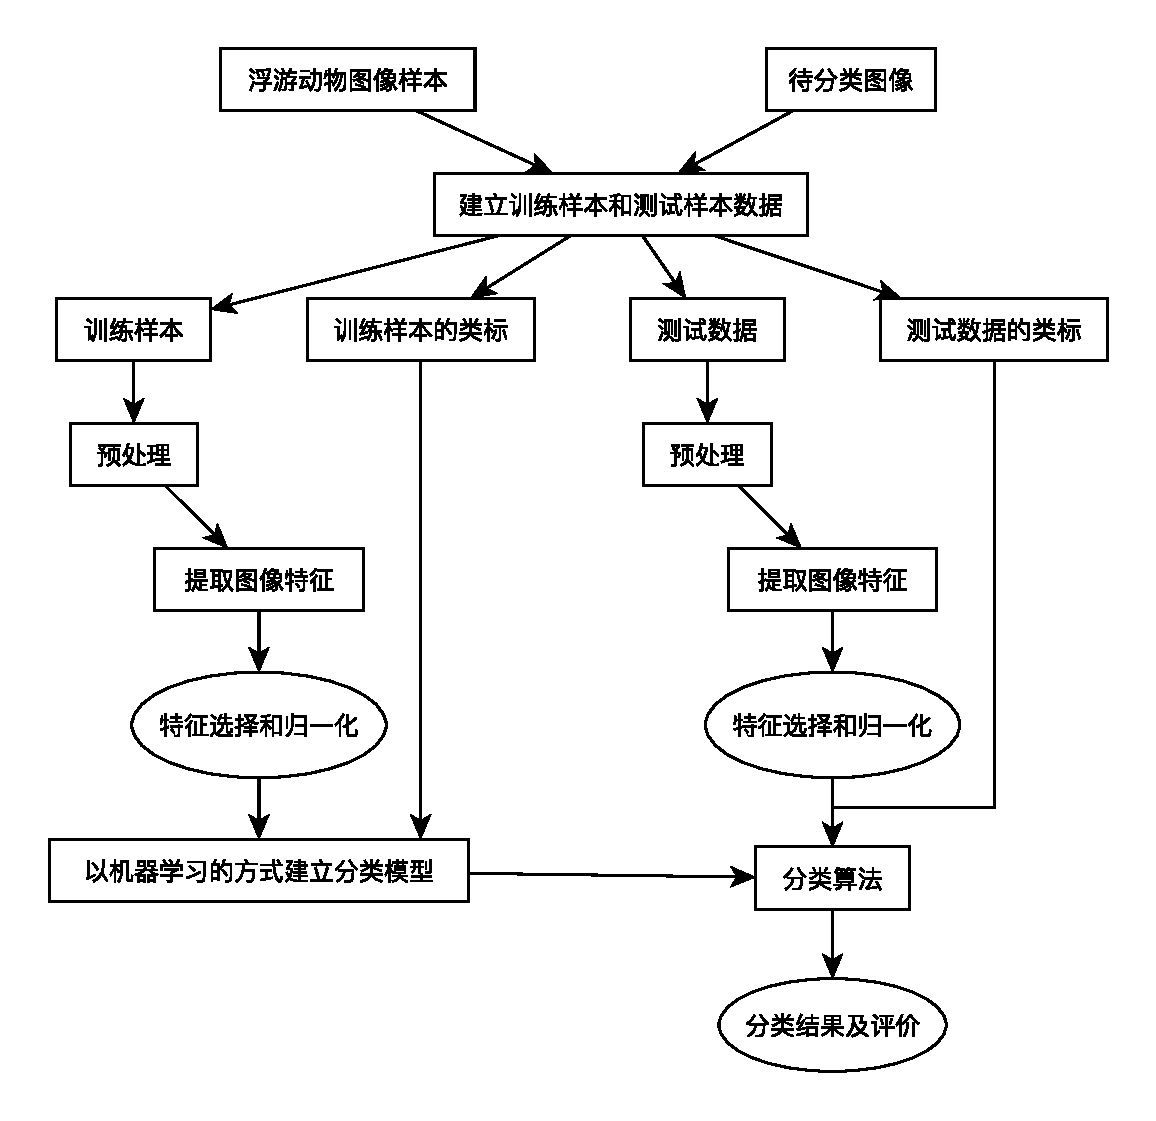
\includegraphics[width=0.6\textwidth]{ClassificationFlowchart.eps}
\caption{利用机器学习方法实现浮游动物图像分类的基本流程}
\label{fig: ClassificationFlowchart}
\end{figure}

\section{数据集}
\label{2.1}

自1949年起,加利福尼亚海洋渔业研究合作组织(California Cooperative Oceanic Fishery Investigation, CalCOFI)就开始对包括浮游生物在内的海洋生物进行采样~\cite{bograd2003calcofi},根据标准邦戈网络协议采集海洋中的浮游生物样本,然后立即保存起来。部分被保存的CalCOFI样本被连接到加利福尼亚对当前生态系统进行长期生态研究的网站上,并用ZooScan进行了扫描~\cite{gorsky2010digital}。得到的灰度图像质量较好,在对比度、噪声等方面都得到了精确控制。整个数据集包含的种类如表~\ref{表1}所示,其中每种类别图像所占比例见图~\ref{fig: ratio},以下对该数据集中的每一类别分别进行了详细说明和描述。

\begin{table}[htbp]
\centering
\caption{浮游动物数据集包含种类}
\begin{tabular}{|r|l|}
\hline
Appendicularia & 尾海鞘纲 \\
Bubble & 气泡 \\ 
Chaetognatha & 毛颚动物门 \\
Cladocera Penilia & 尖头溞属 \\
Copepoda & 桡脚类 \\
Decapoda & 十足目 \\
Doliolida & 海樽目 \\
Egg & 卵 \\
Fiber & 纤维 \\
Gelatinous & 明胶 \\
Multiple & 多个生物 \\
Pteropoda & 翼足目 \\
Nonbio & 非生物 \\
\hline
\end{tabular}
\label{表1}
\end{table}

\begin{figure}[!ht]
\centering
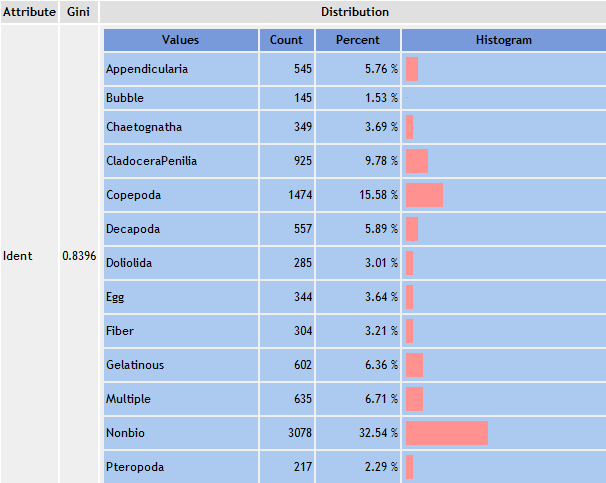
\includegraphics[width=0.6\textwidth]{每个类别所占比例.png}
\caption{数据集中每种类别的数目及所占比例}
\label{fig: ratio}
\end{figure} 

\begin{description}
    \item[Appendicularia(尾海鞘纲)] 属于脊索动物门,体型像蝌蚪,身体分为躯干和尾两部分。躯干较大且灰度较深,呈不太规则的椭圆形。尾部比躯干要长,长度大多小于5mm。尾部大致呈现两种形状:一种细长弯曲,另一种较粗(粗细甚至于头部差不多),呈现柳叶状。尾部的灰度相比于躯干较浅,轮廓不太清晰。

    \item[Bubble(气泡)] 非生物,圆形。气泡四周灰度深,中间灰度很浅,呈亮白色。

    \item[Chaetognatha(毛颚动物门)] 身体修长,可以明显看出身体分为头、躯干和尾3部分。头部略膨大,躯干与头连接处稍微缢缩为颈部,躯干较粗,轮廓清晰。尾部慢慢变窄,末端尖细。头部两侧各着生一列4~13根镰刀状、几丁质的颚毛。大小:最大成年成年个体长105mm,该类成年个体的长度一般都大于5mm。

    \item[Cladocera Penilia(Penilia,尖头溞属)] 属于节肢动物门,鳃足纲,枝角目,俗称水跳蚤。身体短小,有两条长长的触角。该类浮游动物身体中轴线的地方灰度较深(感觉类似人体的脊柱),这个颜色较深的中轴线上还有一条条纹理线连向边缘(就像人体脊柱上连着的骨骼)。由于运动,扫描得到的图像中浮游动物的中轴线并不是都在其身体中间。大小约为1mm左右。
    
    \item[Copepoda(桡脚类)] 属于节肢动物门,颚足纲,桡足类属于其下的一个亚纲。体形像泪珠,有大的触角。分为前体部和后体部,前体部较为宽大,后体部较为短小。前体部前体部由头和胸部组成,头部有两对触角,胸部有鄂足、五对胸足。后体部无附肢,由3—5节组成。最末的腹节称尾节,末端具1对尾叉,尾叉的末端有5根不等长的刚毛,常呈羽状。    
    
    \item[Decapoda(十足目)] 属于节肢动物门,软甲纲。又分为两类:Lucifer hanseni和Crab larvae。体躯延长呈虾形(腹部发达)或缩短扁圆呈蟹形(腹部化)。

    \item[Doliolida(海樽目)] 属于脊索动物门,樽海鞘纲。体型一般呈桶状,体壁最外是被囊层,其内层是外套膜。被囊层下有8~9条肌带环绕着体躯。由于该类浮游动物比较透明,因此在图像中灰度较浅,并且其桶状轮廓也不完整了,但最明显的是能看到大概7、8条环状的肌肉带,有的图像中还能看到内部器官。

    \item[Egg] 很多种类生物的卵。形状大致都呈圆形。有的卵整体灰度都很深;有的卵中间有一块灰度较深的区域,四周灰度较浅(结构像细胞)。由于是不同动物的卵,因此其灰度特征差异较大。

    \item[Fiber(纤维)] 非生物。弯曲的线状,有的纤维有分叉和交叉。该类图像中噪声较多,纤维的边缘也不是很规则。

    \item[Gelatinous(明胶)] 该类包括很多不同种类的胶状生物,它们体内都含有很高的水分。包括Aglaura(属于刺胞动物门)、Medusa(水母,属于刺胞动物门,水螅纲)、Siphonophora(管水母,属于刺胞动物门,水螅纲,管水母目)、Radiolaria(放射虫,属于原声动物门,辐足纲)和Salps(樽海鞘,属于脊索动物门Chordata,樽海鞘纲Thaliacea,纽鳃樽目Salpida)。其中水母大部分都有三个主要部位:圆伞状或是钟状(寺院里面敲得那种钟)的身体、触器和口腕。由于该类呈胶状,因此该类物体灰度整体较浅,边缘也不是十分清晰。大部分是水母,有小部分的樽海鞘(与海樽目形态很相似),小部分的放射虫。
        \item 其中水母也包括很多类,形态大致呈现以下几种:
            \begin{itemize}
            \item 一些水母身体呈现类似钟状(这里呈现钟状有长有短,有粗有细,还有的会发生一点弯曲),灰度较浅,内部有一块颜色较深的椭圆形区域。
            \item 一些水母也呈钟状,但内部没有颜色较深的椭圆形区域,整个身体灰度均匀。
            \item 还有的个头稍微偏小,形状有的类似圆形、像半个胶囊(应该是由于拍摄原因,有的拍到顶部,有的拍到侧面),体内有颜色较深的一个大点和几个小点。(可能是灯塔水母)
            \end{itemize}
        \item 放射虫:形状近似圆形(但由于整体灰度较浅,形状保存是完整),中间有一块灰度较深的区域,四周灰度较浅,可以看到淡淡的细纹从中心连接到边界。
        
    \item[Multiple(多个生物)] 由于浮游动物的重叠,导致分割过程中多个浮游动物被分割到一张图像上。
    
    \item[Pteropoda(翼足目)] 属于软体动物门,腹足纲。该类浮游动物灰度较深,形状总体都呈现一头宽一头窄。形状总体呈现三类:有的呈现象牙状,有点弯曲;有的较粗短,像一顶尖的小帽子;有的呈现细长的三角形状。
    
     \item[Nonbio] 非生物的集合。
\end{description}

\section{评价方法}

\subsection{混淆矩阵简介}
\label{CM}

在机器学习中,混淆矩阵(CM)是一种比较简单的对分类模型的性能进行评价的评估准则,主要用于比较分类结果和实际测得值。混淆矩阵是一个$n$行$n$列的矩阵,$n$代表类别的数量。矩阵的每一列代表预测的每一类的数量,每一行代表实际的每一类的数量。对角线上表示分类正确的每一类的数量。例如:有180个样本数据,这些数据实际分为3类,每类60个,分类结束后得到的混淆矩阵如表~\ref{ConfusionMatrixExample}所示。第一行说明类1的60个样本有53个样本分类正确,5个错分为类2,2个错分为类3。第一列说明类1有53个样本分类正确,类2的2个样本被错分为类1,类3没有样本被错分为类1。对角线上的数据表示,类1、2、3分别有53、55、59个样本被分类正确。
    
\begin{table}[ht]
\centering
\caption{混淆矩阵例子}
\begin{tabular}[c]{|c|c|c|c|}
\hline
 & 类1 & 类2 & 类3\\
 \hline
类1 & 53 & 5 & 2 \\
\hline
类2 & 2 & 55 & 3\\ 
\hline
类3 & 0 & 1 & 59\\ 
\hline
\end{tabular}
\label{ConfusionMatrixExample}
\end{table}

根据混淆矩阵可以导出以下几个参数:
\begin{itemize}
    \item true positives (TP):正样本被识别出的数量
    \item true negatives (TN):负样本被识别出的数量
    \item false positives (FP):负样本被错误分为正样本的数量
    \item false negatives (FN):正样本被错误分为负样本的数量 
    \item Accuracy:准确率,针对分类器的整个预测情况。
        \begin{displaymath}
            Accuracy=\frac{TP+TN}{TP+TN+FP+FN}
        \end{displaymath}
    \item {Error rate:误分类率,针对分类器的整体预测情况。}
        \begin{displaymath}
            Error rate=\frac{FP+FN}{TP+TN+FP+FN}
        \end{displaymath}
    \item {The true positive rate (TPR) :召回率,正样本被识别出的概率。}(文中和PkID中使用的评价参数)
        \begin{displaymath}
            TPR=\frac{TP}{TP+FN}
        \end{displaymath}
     \item The false positive rate (FPR):虚警率,负样本被错误分为正样本的概率。
        \begin{displaymath}
            FPR=\frac{FP}{FP+TN}
        \end{displaymath}
    \item The true negative rate (TNR):负样本被识别出的概率
        \begin{displaymath}
            TNR=\frac{TN}{FP+TN}
        \end{displaymath}

    \item The false negative rate (FNR) :漏警率,正样本被错误分为负样本的概率。
        \begin{displaymath}
            FNR=\frac{FN}{FN+TP}
        \end{displaymath}
    \item {False discovery rate (FDR):1-precision。}(文中和 PkID 中使用的评价参数)
        \begin{displaymath}
            FDR=\frac{FP}{FP+TP}
        \end{displaymath}
    \item Positive predictive value (PPV)
        \begin{displaymath}
            PPV=\frac{TP}{TP+FP}
        \end{displaymath}
    \item Negative predictive value (NPV)
        \begin{displaymath}
            NPV=\frac{TN}{TN+FN}
        \end{displaymath}
    
\end{itemize}

\subsection{混淆矩阵分类}

根据训练集和测试集的不同选取方式,混淆矩阵可以通过以下两种方式得到:
\begin{enumerate}
\item Re-substitution混淆矩阵       
当采用的测试集和训练集为同一个数据集时,得到的混淆矩阵叫做Re-substitution混淆矩阵。在这个过程中,用产生的分类器对测试集进分类时,得到的分类结果错误较少甚至可能没有错误,在进行评价时就会低估分类器的错误率。
\item 交叉验证混淆矩阵
采用交叉验证(交叉验证介绍见~\ref{Cross Validation})的方法得到的混淆矩阵就叫做交叉验证混淆矩阵。并且这里采用的训练集和测试集之间在样本上是没有重合的。首先将一个数据集分成$K$个相等的子集,用其中$K-1$个子集来训练产生分类器,用剩下的1个子集来进行测试,重复进行$K$次来构建混淆矩阵。
\end{enumerate}

\subsection{交叉验证}
\label{Cross Validation}
交叉验证是用来评价分类器的分类性能的一种方法,其基本步骤是是对原始图像集进行分组,然后选择没有交叉的两部分,一部分用作训练,一部分用作测试,用得到的混淆矩阵来评价分类器的性能好坏。

在机器学习的常见算法中,首要的步骤通常是将数据集分为训练集和测试集两个子集,其中训练集用来建立模型,而测试集则用来评价该模型对未知样本进行预测时的准确度,即泛化能力。如何将完整的数据集分为训练集跟测试集,必须遵守以下几条要点:
\begin{enumerate}
    \item 在训练分类器阶段用到的是训练集,不能使用测试集,训练完成后再在测试集上测试分类效果,将两者在分类器建立前后做到严格分离。
    \item 一般来说,训练集中图像数量要多于测试集,以保证训练出的分类器有效。
    \item 对于训练集和测试集,都必须做到对原始数据中每一类都均匀采样,不能过分偏向其中某几类,这样会导致训练出的分类器没有将所有类别的特点都考虑进去。
\end{enumerate}

常见的交叉验证形式有Holdout验证、$K$折交叉验证和留一验证三种,其中用的比较多是$K$折交叉验证。首先将原始的整个图像集平均分成$K$份,一般是随机挑选分配。每一次训练分别将其中一份作为训练集,另外的$K-1$份作为测试集,得到一个混淆矩阵,由于有$K$份,所以会进行$K$次训练和测试,得到$K$个混淆矩阵,将这$K$个混淆矩阵累加起来,就能得到$K$折交叉验证的混淆矩阵。$K$的取值通常大于等于2。在将图像集分成子集时由于是随机分配的,带有一定的随机性,所以在实际应用中,为了避免随机性对分类器效果的影响,我们通常会随机分配$n$次,将每一次得到的$K$折交叉验证的混淆矩阵进行叠加,得到最终的混淆矩阵。

本文中对分类结果采用$K$折交叉验证方式得到的混淆矩阵进行评价,其中$K$取值为2,$n$取值为5,对混淆矩阵计算Recall和1-Precision值,得到每一类的分类准确率和错误率,再对所有类别求平均,得到对整个数据集进行分类的分类准确率和错误率。

\section{ZooScan系统介绍}

利用机器学习方法进行浮游动物图像分类的方法有很多,目前取得最好的分类效果的是法国国家科学研究院研制的ZooScan系统~\cite{gorsky2010digital},受到该系统的启发,我们对其中的浮游动物图像特征提取和分类器设计两个关键环节进行了更深入的研究,从而对其进行了有效的改进,使分类准确率进一步提高。下面具体介绍ZooScan系统的主要组成部分。

\subsection{简介}

ZooScan Integrated System是由法国国家科学研究院Villefranche海洋实验室的Gorsky等人发明、Hydroptic公司生产的浮游动物样品图像扫描和处理系统,能够快速实现对液体中的浮游动物样品的扫描、计数、种类鉴定和生物量的测定,目前在国内和国外都影响很广。

ZooScan系统是由ZooScan、ZooProcess和Plankton Identifier (PkID)三个部分组成的,其中前者是系统的硬件部分,用来对液体中的浮游动物样品进行扫描,得到高分辨率的数字图像。后两者是软件部分,先对扫描得到的图像进行一些标准化处理,对个体的一些形态、几何、灰度等参数进行提取,然后利用一些基本的机器学习算法对特征进行训练,得到分类器,最终实现对浮游动物图像的分类识别。

\begin{figure}[!ht] %插图
\centering
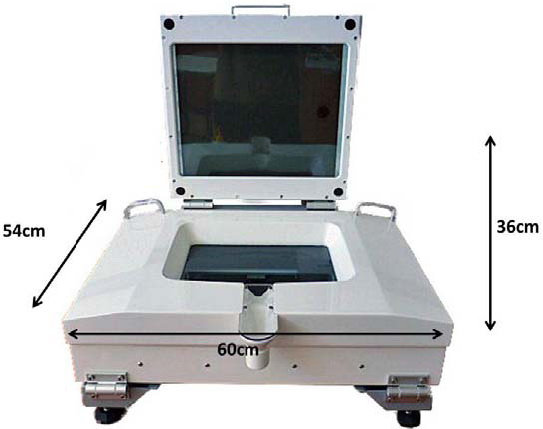
\includegraphics[width=0.4\textwidth]{ZooScan.jpg}
\caption{ZooScan主扫描区}
\label{fig: ZooScan}
\end{figure}

\subsection{硬件部分}

ZooScan系统的扫描设备分为了上下两个部分(图~\ref{fig: ZooScan}),为了能够扫描带液体的样本,对设备的防水性有较高的要求,ZooScan扫描系统在这方面作了很好地处理,其内部隔绝水的性能相当好。扫描设备的上面部分提供了两种功能,一是照明,二是进行光密度的检测。下面部分是扫描区域,即液体样本的放置地方。由于扫描时光是从空气进去水中,再从水中进入玻璃,要分两次完成在两种不同介质之间的穿透,因而在成像效果上会相应差一些,表现为图像分辨率的降低。针对浮游动物样本的不同尺寸,ZooScan系统提供了$1200dpi$和$2400dpi$两种分辨率以及$11cm\times24cm$和$15\times24cm$两种大小的扫描框以供选用。

\begin{figure}[!ht] %插图
\centering
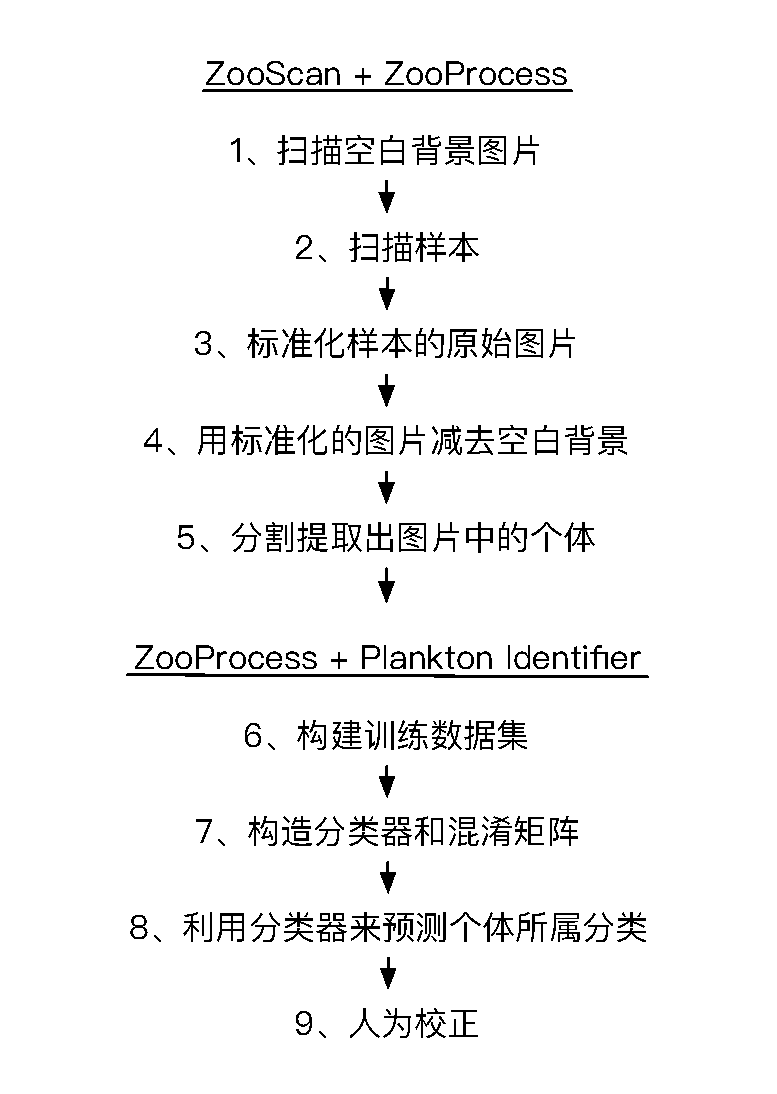
\includegraphics[width=0.4\textwidth]{ZooScanFlowchart.eps}
\caption{利用机器学习方法实现浮游动物图像分类的基本流程}
\label{fig: ZooScanFlowchart}
\end{figure}

\subsection{软件部分}
\label{2.3.3}

利用ZooScan系统对浮游动物进行扫描和分析的基本步骤如图~\ref{fig: ZooScanFlowchart}所示。最初的步骤是使用ZooProcess软件完成:(i)扫描空白背景图片,(ii)扫描样品以获得高质量的原始图片和元数据信息,(iii)标准化原始图片,(iv)去掉扫描框的边缘,以空白背景校正图片,(v)分割提取并测量图片中的个体。随后的分析步骤是利用ZooProcess结合PkID完成:(vi)构建训练数据集,(vii)构造分类器和混淆矩阵,(ix)利用分类器来预测个体所属分类,(x)人为校正。下面会详细说明这些步骤。

\begin{enumerate}
\item 扫描空白背景图片

在扫描空白背景图片前需要打开ZooProcess软件创建一个新的项目,设置扫描参数,有$1200dpi$和$2400dpi$两种分辨率可供选择。然后输入样本的元数据信息。

背景图像是一张空白图像,在与样品相同环境下(自来水或是过滤海水),先扫描背景再扫描样品。并且最好是在每个扫描任务开始时,都扫描一次背景图像。首先用清水清洁和冲ZooScan 托盘和表面玻璃,时不时地检查并清除在玻璃和扫描框上的污点。然后倒一些清水(保持在室温)没过托盘,它可以防止扫描框刮擦托盘。再放置扫描框($15cm \times 24cm$),这取决于之前 ZooProcess 中的“创建项目”中的选项。在预扫描和实际扫描之间,等待 30 秒。

\item 扫描样品以获得高质量的原始图片和元数据信息

首先需要准备好样品,存储几升清水,保持在室温,用来为 ZooScan 注水。然后用筛子(网格间隙为$100\mu m$)过滤掉防腐剂和海水中物质。样品通过间隙为$1mm$和$200\mu m$的两种网格,将浮游生物分成不同体型的两部分。分别将分开后的样品,添加标签$d1$和$d2$,用于扫描后的数据处理过程中。使上述两个分开后的样品中,保持只有 $1000 − 1500$ 个浮游生物。

在扫描托盘中加入量水,放置扫描框($15cm \times 24cm$),调整扫描框放置的位置(位置在扫描托盘中有标注)。倒入样品,加入清水,直到没过扫描框的台阶。将个体较大的浮游生物放在扫描框的中心,用木棒分离粘连浮游生物,避免浮游生物贴靠扫描框边缘。对于漂浮在水面的浮游生物,轻轻用木棒将浮游生物压入水中。如果存在无法没入水中的浮游动物,且数量不多,则将它们移出。检查托盘是否有气泡,顶盖玻璃的表面是否冷凝。加载 ZooProcess,选择项目,点击扫描样品,选择两部分样品中的一个样品($d1$和$d2$)。扫描完成后,输入相关元数据,用于将来的使用和比较。

\item 标准化原始图片

对扫描图片进行标准化可以允许使用不同参数得到的扫描图片之间进行转化和运算。对扫描图片和背景图片都要进行标准化,然后再进行相减操作。其中灰度和尺寸大小是浮游动物自动识别过程的两个最重要的变量,16位的原始图片可以通过计算黑点(Black point, Bp)和白点(White point, Wp)转化为8位图片。
\begin{align}
Wp = Mg \cdot 1.15\\
Bp = \frac{Mg}{1.15 \cdot log(OD)}
\end{align}
其中,Mg(Median grey level)表示图片的平均灰度值,OD表示光密度值。

\item 去掉扫描框的边缘,以空白背景校正图片

对标准化后的原始图片和空白图片进行相减。

\item 分割提取并测量图片中的个体

默认的分割灰度值为243,等周长直径(Equivalent Circular Diameter, ECD)大于$0.3mm$的个体会被检测出来并进行下一步处理。

\item 相关参数提取

ZooProcess中对个体提取的参数一共有67个:Area, Mean, StdDev, Mode, Min, Max, X, Y, XM, YM, Perim., BX, BY, Width, Height, Major, Minor, Angle, Circ., Feret, IntDen, Median, Skew, Kurt, \%Area, XStart, YStart, Area\_exc, Fractal, Skelarea, Slope, Histcum1, Histcum2, Histcum3, XMg5, YMg5, Compentropy, Compmean, Compslope, CompM1, CompM2, CompM3, Symetrieh, Symetriev,Tag, ESD, Elongation, Range, MeanPos, CentroidsD, CV, SR, PerimAreaexc, FeretAreaexc, PerimFeret, PerimMaj, Circexc, CDexc, Nb1, Nb2, Nb3,  Symetriehc, Symetrievc, Convperim, Convarea, Fcons, ThickR。大致可以分为位置特征、尺寸特征、灰度特征、形状特征、生物统计特征、自定义特征六大类。

\begin{enumerate}
\item 位置特征
\begin{description}
\item[BX、BY] 能够包围物体,且平行于图像两条边的最小外界矩形的左上角顶点的X坐标和Y坐标。
\item[Height、Width] 能够包围物体,且平行于图像两条边的最小外界矩形的高和宽。
\item[XStart、YStart] 图像最左上角像素点的X坐标和Y坐标。
\item[XM、YM] 物体灰度重心的X坐标和Y坐标。
\item[XMg5、YMg5] gamma值为51时的物体灰度重心的X坐标和Y坐标(gamma值表示图像输出值与输入值关系的斜率)。
\item[X、Y] 物体重心点的X坐标和Y坐标。
\item[Angle] 浮游动物主轴与图片x轴形成的夹角,在图片切割后旋转图片测量相关参数使用。
\end{description}
这类特征反映的是浮游动物在图像中的位置信息,浮游动物特征与位置信息无关,因此它们不适合作为特征直接用于分类(会降低分类的准确率),而是用来计算其他特征(尺寸特征、灰度特征和形状特征)。

\item 尺寸特征

\begin{description}
\item[Area] 包含物体的最小矩形面积 。
\item[Perim] 周长,物体最外层边缘的长度。
\item[Major] 物体的最佳拟合椭圆的长轴。%物体内切椭圆的长轴
\item[Minor] 物体的最佳拟合椭圆的短轴。%物体内切椭圆的短轴
\item[Feret] Maximum feret diameter(最大费雷特径), 沿物体边缘任意两个点的最长距离。
\item[Area\_exc] 去掉物体空洞后的表面积,空洞是指灰度值与背景相同的部分。
\item[\%area] 物体表面积中空洞所占的百分比,即背景所占的比例。
\end{description}

这类特征表示了图像中目标的大小尺寸。它的根据是同类浮游动物的表面积、周长等尺寸特征应该是大致相同的。但是这些特征还存在着问题:1、同类浮游动物在不同时期(如幼年和成年)的个体大小尺寸是不同的。2、拍摄照片的方位不同(比如正面和侧面),得到的尺寸特征也是不同的。

\item 灰度特征

\begin{description}
    \item[Min、Max] 物体内部所有像素点的最小灰度值和最大灰度值(0 = black,255 = white)。
    \item[IntDen (Integrated density)] 总密度,物体内像素点的灰度值的总和($IntDen = Area * Mean$)。
    \item[Slope] 归一化的灰度累计直方图的斜率。
    \item[Histcum1] 灰度累计直方图的值为25\%时所对应的灰度值。
    \item[Histcum2] 灰度累计直方图的值为50\%时所对应的灰度值。
    \item[Histcum3] 灰度累计直方图的值为75\%时所对应的灰度值。
    \item[CentroidsD] $\sqrt{(XM-X)^{2}+(YM-Y)^{2}}$ 目标物体重心和灰度重心之间的距离。
    \item[Fcons] 灰度对比度。
    \item[Nb1] 图像在用阈值Histcum1二值化后剩余对象的数量。
    \item[Nb2] 图像在用阈值Histcum2二值化后剩余对象的数量。
    \item[Nb3] 图像在用阈值Histcum3二值化后剩余对象的数量。
    \item[ThickR] 物体最大厚度和平均厚度(不包括最大厚度)的比值。
\end{description}

利用灰度特征进行浮游动物图像分类的依据是同类浮游动物的灰度特征(灰度的范围和整体灰度变换趋势)应该是相似的。但观察图像发现并不是所有同类浮游动物的灰度都是相似的,例如Gelatinous类中有的个体灰度跨度较小,整体灰度都较浅,而有的个体灰度跨度较大。同时由于拍摄时光线的原因,也会造成同类浮游动物中个体灰度的深浅不一。

\item 形状特征

\begin{description}
    \item[Fractal] 物体边界的分形维数,表明物体边界的不规则程度。
    \item[Skelarea] 骨架像素的表面积(在二值图像中,不断地从物体边缘处减去像素点直到仅剩一个像素的宽度,最后所得图形的像素点数)。
    \item[Symetrieh] 关于水平轴的对称性。
    \item[Symetriev] 关于竖直轴的对称性。
    \item[Symetriehc] 图像在用阈值Histcum1二值化后物体的水平对称性。
    \item[Symetrievc] 图像在用阈值Histcum1二值化后物体的垂直对称性。
    \item[Circ] $Circularity = (4 * Pi * Area) / Perim^2$ 圆形度,表征物体接近圆的程度,值等于1时,说明物体为正圆形,值越接近0,物体体形越长。
    \item[ESD] $2 \times \sqrt{\cfrac{Area}{\pi}}$ 相应球形直径(也称为等效球直径),是指一不规则外形物体,其体积相同球体的直径。
    \item[Elongation] $\cfrac{Major}{Minor}$ 延伸率,最佳拟合椭圆的长轴和短轴之比。
    \item[Circexc] $\cfrac{4 \times \pi Area\_exc}{Perim^{2}}$ 去掉目标内部空洞的圆形度。
    \item[Convperim] 包围物体凸包的周长。
    \item[Convarea] 包围物体凸包的面积。
\end{description}

这类特征描述的是浮游动物的形状特征,依据是不同种类浮游动物之间形状不同。但在本文所采用的数据集中存在的问题是有不同种类的浮游动物形状相似,例如Appendicularia和Chaetognatha,Bubble和Egg,也有同种浮游动物形状不同,例如Decapoda、Gelatinous。

\item 生物统计特征

\begin{description}
    \item[Mean] 物体内的平均灰度值,物体中所有像素点的灰度值的总和除以总的像素个数。
    \item[Range] $Max-Min$ 极差,灰度的范围。    
    \item[CV] $100 \times \cfrac{StdDev}{Mean}$ 变异系数(也称离散系数或相对偏差),是灰度标准偏差与平均值之比,用百分数表示。
    \item[SR] $100 \times \cfrac{StdDev}{Max-Min}$ 灰度标准差比上极差。
    \item[Skew] 灰度直方图的偏度,衡量灰度分布的不对称性。正态分布的偏度为0,概率密度函数两侧的尾部长度互相对称。偏度为负表示概率密度函数左侧的尾部相对于右侧要长,大部分的值位于平均值的右侧。偏度为正表示概率密度函数右侧的尾部比左侧的长,即处于平均值左侧的值要比右侧多。
    \item[Kurt] 峰度,描述灰度直方图的陡缓程度。 
    \item[Mean\_exc] 物体内部去掉空洞后的平均灰度值($Mean\_exc = IntDen / Area\_exc$)。
    \item[Median] 物体内像素的灰度值的中值。
    \item[StdDev] 物体内像素的灰度值的标准差。
    \item[Mode] 表示灰度的众数。
\end{description}

\item 自定义特征
\begin{description}
    \item[MeanPos] $\cfrac{Mean-Max}{Max-Min}$
    \item[PerimAreaexc] $\cfrac{Perim}{\sqrt{Area\_exc}}$ 
    \item[FeretAreaexc] $\cfrac{Feret}{\sqrt{Area\_exc}}$
    \item[PerimFeret] $\cfrac{Perim}{Feret}$
    \item[PerimMaj] $\cfrac{Perim}{Major}$
    \item[CDexc] $\cfrac{\sqrt{(XM-X)^{2}+(YM-Y)^{2}}}{{\sqrt{Area\_exc}}}$ 
    \item[ESD] $2 \times \sqrt{\cfrac{Area}{\pi}}$
    \item[Elongation] $\cfrac{Major}{Minor}$
    \item[Range] $Max-Min$
    \item[CentrodisD] $\sqrt{(XM-X)^{2}+(YM-Y)^{2}}$
    \item[CV] $100 \times \cfrac{StdDev}{Mean}$
    \item[SR] $100 \times \cfrac{StdDev}{Max-Min}$
    \item[Circexc] $\cfrac{4 \times \pi Area\_exc}{Perim^{2}}$
\end{description}
\end{enumerate}
\end{enumerate}
%
%
% %%% 其它部分
% \backmatter
% % 插图索引
% \listoffigures
% % 表格索引
% \listoftables
% % 公式索引
% \listofequations
%
%
% % 参考文献
% \bibliographystyle{thubib}
% \bibliography{ref/refs}
%
%
% % 致谢
% %%% Local Variables:
%%% mode: latex
%%% TeX-master: "../main"
%%% End:

\begin{ack}
时光匆匆如流水,转眼便又是毕业时节了,在我三年的硕士研究生生涯里,我所收获的不仅仅是愈加丰厚的知识,更重要的是思维方式和表达能力的转变与提升。我很庆幸在这三年我遇到了很多的良师益友,无论在学习上、生活上还是工作上,都给予了我无私的帮助和悉心的照顾,让我在一个温馨、有爱的环境中度过了我的三年研究生生活。

首先,我要感谢我的导师郑海永,这三年来给我最多教育和帮助的人!从我开始读研开始,郑老师一直对我严格要求,在他的指导下,我不仅树立了远大的学习目标,掌握了基本的研究方法,还明白了很多为人处世的道理。本论文从选题到最终完成,每一步都得到了郑老师的帮助和指点,在我迷茫时给予适时的鼓励,帮助我开拓研究思路,解决问题。感谢师母冯丽颖的关怀和教育,使我认识到自身的不足,从而努力提高自己,做一个坚强、会生活、懂生活的新时代女性。在此,谨向导师和师母表示崇高的敬意和衷心的感谢!

感谢实验室所有兄弟姐妹,没有你们的陪伴,我不会拥有这么美好、难忘的三年回忆。感谢我的师姐赵红苗、师妹王如晨,和我并肩作战,在我的研究课题上给予了很多的支持和帮助,让我有了更大提高。

感谢我的家人,谢谢你们无私的付出,在我身后坚定地支持我、关心我、帮助我,有你们在,我更安心!

感谢国家自然科学基金青年科学基金项目“基于视觉注意结合生物形态特征的海洋浮游植物显微图像分析”(批准号:61301240)、国家自然科学基金项目“基于生物形态特征的中国海常见有害赤潮藻显微图像识别”(批准号:61271406)和中央高校基本科研业务费“海洋浮游动物原位探测与分析系统”(批准号:201562023)的资助。

最后,感谢所有关心和帮助过我的人,祝愿你们幸福安康!
\end{ack}

%
% % 附录
% \begin{appendix}
% %%% Local Variables: 
%%% mode: latex
%%% TeX-master: "../main"
%%% End: 

\chapter{}
\label{}

\chapter{}
\section{}

\chapter{}


% \end{appendix}
%
% % 个人简历
% \begin{resume}

  \resumeitem{个人简历}

  1990 年 9 月 4 日出生于 江苏 省 泰州 市 姜堰 区。
  
  2009 年 9 月考入 中国海洋大学 电子工程系 电子信息科学与技术 专业,2013 年 6 月本科毕业并获得 理学 学士学位。
  
  2013 年 9 月考入 中国海洋大学 电子 系攻读 硕士 学位至今。

  \resumeitem{发表的学术论文} % 发表的和录用的合在一起
     
  \begin{enumerate}[{[}1{]}]
  \item Wang X, Dai J, Zhu Y, Zheng H and Qiao X. Spectral saliency via automatic adaptive amplitude spectrum analysis. Journal of Electronic Imaging, 2016. (SCI 收录)
  \item Zhu Y, Chang L, Dai J, Zheng H, Zheng B. Automatic object detection and segmentation from underwater images via saliency-based region merging. Proceedings of OCEANS 2016 MTS/IEEE Shanghai, 2016. (EI 收录)
  \end{enumerate}

  \resumeitem{在学期间参加的研究项目} % 有就写,没有就删除
  \begin{enumerate}
  \item 国家自然科学基金青年科学基金项目“基于视觉注意结合生物形态特征的海洋浮游植物显微图像分析”(批准号:61301240)
  \item 国家自然科学基金项目“基于生物形态特征的中国海常见有害赤潮藻显微图像识别”(批准号:61271406)
  \item 中央高校基本科研业务费“海洋浮游动物原位探测与分析系统”(批准号:201562023)
  \end{enumerate}
  
\end{resume}

%
% \end{document}
% \end{example}
%
% \subsection{选项}
% \label{sec:option}
% 本模板提供了一些选项以方便使用:
% \begin{description}
% \item[bachelor]
%   如果写本科论文将此选项打开。
%   \begin{example}
% \documentclass[bachelor]{thuthesis}
%   \end{example}
%
% \item[master]
%   如果写硕士论文将此选项打开。
%   \begin{example}
% \documentclass[master]{thuthesis}
%   \end{example}
%
% \item[doctor]
%   如果写博士论文将此选项打开。
%   \begin{example}
% \documentclass[doctor]{thuthesis}
%   \end{example}
%
% \item[postdoctor]
%   如果写博士博士后出站报告将此选项打开。
%   \begin{example}
% \documentclass[postdoctor]{thuthesis}
%   \end{example}
%
% \item[secret]
%   涉秘论文开关。配合另外两个命令 \cs{secretlevel} 和 \cs{secretyear} 分别用来指
%   定保密级别和时间。二者默认分别为\textbf{秘密}和当前年份。可以通
%   过:|\secretlevel{绝密}| 和 |\secretyear}{1984}| 修改。
%   \begin{example}
% \documentclass[bachelor, secret]{thuthesis}
%   \end{example}
%
% \changes{v3.0}{2007/05/12}{不用专门为本科论文生成\textbf{提交}版本了。}
%
% \item[openany, openright]
%   正规出版物的章节出现在奇数页,也就是右手边的页面,这就是 \option{openright},
%   也是 \thuthesis\ 的默认选项。在这种情况下,如果前一章的最后一页也是奇数,那么
%   模板会自动生成一个纯粹的空白页,很多人不是很习惯这种方式,而且学校的格式似乎
%   更倾向于页面连续,那就是通常所说的 \option{openany}。{\fangsong 目前所有论文
%   都是 \option{openany}。}这两个选项不用专门设置,\thuthesis{} 会根据当前论文类
%   型自动选择。
%
% \item[winfonts, adobefonts, nofonts]
%   这些选项用来指导 \pkg{ctex} 宏包/文档类设置选用的中文字体。
%   \begin{itemize}
%   \item \option{winfonts} 指定使用中易的六款字体(Xe\TeX 下为四种)。
%   \item \option{adobefonts} 指定使用 Adobe 的四款免费中文字体。
%   \item \option{nofonts} 不提供可用的中文字体,由用户自行设定。
%   \end{itemize}
%
% \item[arial]
%   使用真正的 \option{arial} 字体。此选项会装载 \pkg{arial} 字体宏包,如果此宏包
%   不存在,就装
%   载 \pkg{Helvet}。\option{arialtoc} 和 \option{arialtitle} 不受
%   \texttt{arial} 的影响。因为一般的 \TeX{} 发行都没有 \pkg{arial} 字体,所以默
%   认采用 \pkg{Helvet},二者效果非常相似。如果一定要用 \pkg{arial} 字体,请参
%   看:\href{http://www.mail-archive.com/ctan-ann@dante.de/msg00627.html}{Arial
%   字体}。
%
% \item[arialtoc]
%   目录项(章目录项除外)中的英文是否用 \option{arial} 字体。本选项
%   和 \option{arialtitle} 都不用用户干预,模板根据当前论文类型自动设置。
%
% \item[arialtitle]
%   章节标题中英文是否用 \option{arial} 字体(默认打开)。
% \end{description}
%
% \subsection{字体配置}
% \label{sec:font-config}
% 正确配置中文字体是使用模板的第一步。模板调用 \pkg{ctex} 宏包,提供如下字体使用方式:
% \begin{itemize}
%   \item 基于传统 \pkg{CJK} 包,使用 latex、pdflatex 编译;
%   \item 基于 \pkg{xeCJK} 包,使用 xelatex 编译。
% \end{itemize}
%
% 第一种方式的字体配置比较繁琐,建议使用 \emph{donated@newsmth} 制作的中文字体包
% (自包含安装方法),请用户自行下载安装,此处不再赘述。本模板推荐使用第二种方法,
% 只要把所需字体放入系统字体文件夹(也可以指定自定义文件夹)即可。用户可以使
% 用 \option{winfonts},\option{adobefonts},\option{nofonts} 选项来选择可用的中
% 文字库,缺省为 \option{winfonts} 有效,使用中易字体。当使用 xelatex 编译
% 时,\option{winfonts} 只有中易的四款字体(宋体、黑体、楷书和仿宋)可用,而本科
% 生需要用到幼圆,另外 Linux 系统缺少上述字体,这些用户可以通过指
% 定 \option{nofonts} 选项,利用 \file{thufonts.def} 文件配置所需字体。使用中易
% 六种字体的配置如下:
% \begin{example}
% \ProvidesFile{thufonts.def}
% \setCJKmainfont[BoldFont={SimHei},ItalicFont={KaiTi}]{SimSun}
% \setCJKsansfont{SimHei}
% \setCJKmonofont{FangSong}
% \setCJKfamilyfont{zhsong}{SimSun}
% \setCJKfamilyfont{zhhei}{SimHei}
% \setCJKfamilyfont{zhkai}{KaiTi}
% \setCJKfamilyfont{zhfs}{FangSong}
% \setCJKfamilyfont{zhli}{LiSu}
% \setCJKfamilyfont{zhyou}{YouYuan}
% \newcommand*{\songti}{\CJKfamily{zhsong}} % 宋体
% \newcommand*{\heiti}{\CJKfamily{zhhei}}   % 黑体
% \newcommand*{\kaishu}{\CJKfamily{zhkai}}  % 楷书
% \newcommand*{\fangsong}{\CJKfamily{zhfs}} % 仿宋
% \newcommand*{\lishu}{\CJKfamily{zhli}}    % 隶书
% \newcommand*{\youyuan}{\CJKfamily{zhyou}} % 幼圆
% \end{example}
%
% 对 Windows XP 来说如下,|KaiTi| 需要替换为 |KaiTi_GB2312|,|FangSong| 需要替换
% 为 |FangSong_GB2312|。
%
% 宏包中包含了 \file{zhfonts.py} 脚本,为 Linux/Mac 用户提供一种交互式的方式从系
% 统中文字体中选择合适的六种字体,最终生成对应的 \file{thufonts.def}文件。要使用
% 它,只需在命令行输入该脚本的完整路径即可。
%
% 另外,用户也可以通过命令
% \begin{shell}
% $ fs-list :lang=zh > zhfonts.txt
% \end{shell}
% 得到系统中现有的中文字体列表,并相应替换上述配置。
%
% \subsection{命令}
% \label{sec:command}
% 模板中的命令分为两类:一是格式控制,二是内容替换。格式控制如字体、字号、字距和
% 行距。内容替换如姓名、院系、专业、致谢等等。其中内容替换命令居多,而且主要集中
% 在封面上,其中有以本科论文为最(比硕士和博士论文多了\textbf{综合论文训练任务书}一
% 页)。首先来看格式控制命令。
%
% \subsubsection{基本控制命令}
% \label{sec:basiccom}
%
% \myentry{字体}
% \DescribeMacro{\songti}
% \DescribeMacro{\fangsong}
% \DescribeMacro{\heiti}
% \DescribeMacro{\kaishu}
% \DescribeMacro{\lishu}
% \DescribeMacro{\youyuan}
% 等分别用来切换宋体、仿宋、黑体、楷体、隶书和幼圆字体。
%
% \begin{example}
% {\songti 乾:元,亨,利贞}
% {\fangsong 初九,潜龙勿用}
% {\heiti 九二,见龙在田,利见大人}
% {\kaishu 九三,君子终日乾乾,夕惕若,厉,无咎}
% {\lishu 九四,或跃在渊,无咎}
% {\heiti 九五,飞龙在天,利见大人}
% {\songti 上九,亢龙有悔}
% {\youyuan 用九,见群龙无首,吉}
% \end{example}
%
% \myentry{字号}
% \DescribeMacro{\chuhao}
% 等命令定义一组字体大小,分别为:
%
% \begin{center}
% \begin{tabular}{lllll}
% \hline
% |\chuhao|&|\xiaochu|&|\yihao|&|\xiaoyi| &\\
% |\erhao|&|\xiaoer|&|\sanhao|&|\xiaosan|&\\
% |\sihao|& |\banxiaosi|&|\xiaosi|&|\dawu|&|\wuhao|\\
% |\xiaowu|&|\liuhao|&|\xiaoliu|&|\qihao|& |\bahao|\\\hline
% \end{tabular}
% \end{center}
%
% 使用方法为:\cs{command}\oarg{num},其中 |command| 为字号命令,|num| 为行距。比
% 如 |\xiaosi[1.5]| 表示选择小四字体,行距 1.5 倍。写作指南要求表格中的字体
% 是 \cs{dawu},模板已经设置好了。
%
% \begin{example}
% {\erhao 二号 \sanhao 三号 \sihao 四号  \qihao 七号}
% \end{example}
%
% \myentry{密级}
% \DescribeMacro{\secretlevel}
% \DescribeMacro{\secretyear}
% 定义秘密级别和年限:
%   \begin{example}
% \secretyear{5}
% \secretlevel{内部}
%   \end{example}
%
% \myentry{引用方式}
% \DescribeMacro{\onlinecite}

% 学校要求的参考文献引用有两种模式:(1)上标模式。比如``同样的工作有很
% 多$^{[1,2]}$\ldots''。(2)正文模式。比如``文[3] 中详细说明了\ldots''。其中上标
% 模式使用远比正文模式频繁,所以为了符合使用习惯,上标模式仍然用常规
% 的 |\cite{key}|,而 |\onlinecite{key}| 则用来生成正文模式。
%
% 关于参考文献模板推荐使用 \BibTeX{},关于中文参考文献需要额外增加一个 Entry: lang,将其设置为 \texttt{zh}
% 用来指示此参考文献为中文,以便 thubib.bst 处理。如:
% \begin{example}
% @INPROCEEDINGS{cnproceed,
%   author    = {王重阳 and 黄药师 and 欧阳峰 and 洪七公 and 段皇帝},
%   title     = {武林高手从入门到精通},
%   booktitle = {第~$N$~次华山论剑},
%   year      = 2006,
%   address   = {西安, 中国},
%   month     = sep,
%   lang      = "zh",
% }
%
% @ARTICLE{cnarticle,
%   AUTHOR  = "贾宝玉 and 林黛玉 and 薛宝钗 and 贾探春",
%   TITLE   = "论刘姥姥食量大如牛之现实意义",
%   JOURNAL = "红楼梦杂谈",
%   PAGES   = "260--266",
%   VOLUME  = "224",
%   YEAR    = "1800",
%   LANG    = "zh",
% }
% \end{example}
%
% \myentry{书脊}
% \DescribeMacro{\shuji}
% 生成装订的书脊,为竖排格式,默认参数为论文中文题目。如果中文题目中没有英文字母,
% 那么直接调用此命令即可。否则,就要像例子里面那样做一些微调(参看模板自带
% 的 \file{shuji.tex})。下面是一个列子:
% \begin{example}
% \documentclass[bachelor]{thuthesis}
% \begin{document}
% \ctitle{论文中文题目}
% \cauthor{中文姓名}
% % \shuji 命令需要上面两个变量
% \shuji
%
% % 如果你的中文标题中有英文,那可以指定:
% \shuji[清华大学~\hspace{0.2em}\raisebox{2pt}{\LaTeX}%
% \hspace{-0.25em} 论文模板 \hspace{0.1em}\raisebox{2pt}%
% {v\version}\hspace{-0.25em}样例]
% \end{document}
% \end{example}
%
% \myentry{破折号}
% \DescribeMacro{\pozhehao}
% 中文破折号在 CJK-\LaTeX\ 里没有很好的处理,我们平时输入的都是两个小短线,比如这
% 样,{\heiti 中国——中华人民共和国}。这不符合中文习惯。所以这里定义了一个命令生成更
% 好看的破折号,不过这似乎不是一个好的解决办法。有同学说不能用在 \cs{section} 等命
% 令中使用,简单的办法是可以提供一个不带破折号的段标题:\cs{section}\oarg{没有破
%   折号精简标题}\marg{带破折号的标题}。
%
%
% \subsubsection{封面命令}
% \label{sec:titlepage}
% 下面是内容替换命令,其中以 |c| 开头的命令跟中文相关,|e| 开头则为对应的英文。这
% 部分的命令数目虽然比较多,实际上都相当简单,套用即可。
%
% 大多数命令的使用方法都是: \cs{command}\marg{arg},例外者将具体指出。这些命令都
% 在示例文档的 \file{data/cover.tex} 中。
%
% \myentry{论文标题}
% \DescribeMacro{\ctitle}
% \DescribeMacro{\etitle}
% \begin{example}
% \ctitle{论文中文题目}
% \etitle{Thesis English Title}
% \end{example}
%
% \myentry{作者姓名}
% \DescribeMacro{\cauthor}
% \DescribeMacro{\eauthor}
% \begin{example}
% \cauthor{中文姓名}
% \eauthor{Your name in PinYin}
% \end{example}
%
% \myentry{申请学位名称}
% \DescribeMacro{\cdegree}
% \DescribeMacro{\edegree}
% \begin{example}
% \cdegree{您要申请什么学位}
% \edegree{degree in English}
% \end{example}
%
% \myentry{院系名称}
% \DescribeMacro{\cdepartment}
% \DescribeMacro{\edepartment}
%
% \cs{cdepartment} 可以加一个可选参数,如:\cs{cdepartmentl}\oarg{精简}\marg{详
%   细},主要针对本科生的\textbf{综合论文训练}部分,因为需要填写的空间有限,最好
% 给出一个详细和精简院系名称,如\textbf{计算机科学与技术}和\textbf{计算机}。
% \begin{example}
% \cdepartment[系名简称]{系名全称}
% \edepartment{Department}
% \end{example}
%
% \myentry{专业名称}
% \DescribeMacro{\cmajor}
% \DescribeMacro{\emajor}
% \begin{example}
% \cmajor{专业名称}
% \emajor{Major in English}
% \end{example}
%
% \DescribeMacro{\cfirstdiscipline}
% \DescribeMacro{\cseconddiscipline}
% \begin{example}
% \cfirstdiscipline{博士后一级学科}
% \cseconddiscipline{博士后二级学科}
% \end{example}
%
% \myentry{导师姓名}
% \DescribeMacro{\csupervisor}
% \DescribeMacro{\esupervisor}
% \begin{example}
% \csupervisor{导师~教授}
% \esupervisor{Supervisor}
% \end{example}
%
% \myentry{副导师姓名}
% \DescribeMacro{\cassosupervisor}
% \DescribeMacro{\eassosupervisor}
% 本科生的辅导教师,硕士的副指导教师。
% \begin{example}
% \cassosupervisor{副导师~副教授}
% \eassosupervisor{Small Boss}
% \end{example}
%
% \myentry{联合导师}
% \DescribeMacro{\ccosupervisor}
% \DescribeMacro{\ecosupervisor}
% 硕士生联合指导教师,博士生联合导师。
% \begin{example}
% \ccosupervisor{联合导师~教授}
% \ecosupervisor{Tiny Boss}
% \end{example}
%
% \myentry{论文成文日期}
% \DescribeMacro{\cdate}
% \DescribeMacro{\edate}
% \DescribeMacro{\postdoctordate}
% 默认为当前时间,也可以自己指定。
% \begin{example}
% \cdate{中文日期}
% \edate{English Date}
% \postdoctordate{2009年7月——2011年7月} % 博士后研究起止日期
% \end{example}
%
% \myentry{博士后封面其它参数}
% \DescribeMacro{\catalognumber}
% \DescribeMacro{\udc}
% \DescribeMacro{\id}
% \begin{example}
% \catalognumber{分类号}
% \udc{udc}
% \id{编号}
% \end{example}
%
% \myentry{摘要}
% \DescribeEnv{cabstract}
% \DescribeEnv{eabstract}
% \begin{example}
% \begin{cabstract}
%  摘要请写在这里...
% \end{cabstract}
% \begin{eabstract}
%  Here comes English abstract...
% \end{eabstract}
% \end{example}
%
% \myentry{关键词}
% \DescribeMacro{\ckeywords}
% \DescribeMacro{\ekeywords}
% 关键词用英文逗号分割写入相应的命令中,模板会解析各关键词并生成符合不同论文格式
% 要求的关键词格式。
% \begin{example}
% \ckeywords{关键词 1, 关键词 2}
% \ekeywords{keyword 1, keyword 2}
% \end{example}
%
% \subsubsection{其它部分}
% \label{sec:otherparts}
% 论文其它主要部分命令:
%
% \myentry{符号对照表}
% \DescribeEnv{denotation}
% 主要符号表环境。简单定义的一个 \texttt{list},跟 \texttt{description} 非常类似,
% 使用方法参见示例文件。带一个可选参数,用来指定符号列的宽度(默认为 2.5cm)。
% \begin{example}
% \begin{denotation}
%   \item[E] 能量
%   \item[m] 质量
%   \item[c] 光速
% \end{denotation}
% \end{example}
%
% 如果你觉得符号列的宽度不满意,那可以这样来调整:
% \begin{example}
% \begin{denotation}[1.5cm] % 设置为 1.5cm
%   \item[E] 能量
%   \item[m] 质量
%   \item[c] 光速
% \end{denotation}
% \end{example}
%
% \myentry{索引}
% 插图、表格和公式三个索引命令分别如下,将其插入到期望的位置即可(带星号的命令表
% 示对应的索引表不会出现在目录中):
%
% \begin{center}
% \begin{tabular}{ll}
% \hline
%   {\heiti 命令} & {\heiti 说明} \\\hline
% \cs{listoffigures} & 插图索引\\
% \cs{listoffigures*} & \\\hline
% \cs{listoftables} & 表格索引\\
% \cs{listoftables*} & \\\hline
% \cs{listofequations} & 公式索引\\
% \cs{listofequations*} & \\\hline
% \end{tabular}
% \end{center}
%
% \LaTeX{} 默认支持插图和表格索引,是通过 \cs{caption} 命令完成的,因此它们必须出
% 现在浮动环境中,否则不被计数。
%
% 有的同学不想让某个表格或者图片出现在索引里面,那么请使用命令 \cs{caption*},这
% 个命令不会给表格编号,也就是出来的只有标题文字而没有``表~xx'',``图~xx'',否则
% 索引里面序号不连续就显得不伦不类,这也是 \LaTeX{} 里星号命令默认的规则。
%
% 有这种需求的多是本科同学的英文资料翻译部分,如果你觉得附录中英文原文中的表格和
% 图片显示成``表''和``图''很不协调的话,一个很好的办法还是用 \cs{caption*},参数
% 随便自己写,具体用法请参看示例文档。
%
% 如果你的确想让它编号,但又不想让它出现在索引中的话,那就自己改一改模板的代码吧,
% 我目前不打算给模板增加这种另类命令。
%
% 公式索引为本模板扩展,模板扩展了 \pkg{amsmath} 几个内部命令,使得公式编号样式和
% 自动索引功能非常方便。一般来说,你用到的所有数学环境编号都没问题了,这个可以参
% 看示例文档。如果你有个非常特殊的数学环境需要加入公式索引,那么请使
% 用 \cs{equcaption}\marg{编号}。此命令表示 equation caption,带一个参数,即显示
% 在索引中的编号。因为公式与图表不同,我们很少给一个公式附加一个标题,之所以起这
% 么个名字是因为图表就是通过 \cs{caption} 加入索引的,\cs{equcaption} 完全就是为
% 了生成公式列表,不产生什么标题。
%
% 使用方法如下。假如有一个非 equation 数学环境 mymath,只要在其中写一
% 句 \cs{equcaption} 就可以将它加入公式列表。
% \begin{example}
% \begin{mymath}
%   \label{eq:emc2}\equcaption{\ref{eq:emc2}}
%   E=mc^2
% \end{mymath}
% \end{example}
%
% 当然 mymath 正文中公式的编号需要你自己来做。
%
% 同图表一样,附录中的公式有时候也不希望它跟全文统一编号,而且不希望它出现在公式
% 索引中,目前的解决办法就是利用 \cs{tag*}\marg{公式编号} 来解决。用法很简单,此
% 处不再罗嗦,实例请参看示例文档附录 A 的前两个公式。
%
% \myentry{简历}
% \DescribeEnv{resume}\DescribeMacro{\resumeitem}
% 开启个人简历章节,包括发表文章列表等。其实就是一个 chapter。里面的每个子项目请用命令 |\resumeitem{sub title}|。
%
% 这里就不再列举例子了,请参看示例文档的 data/resume.tex。
%
% \myentry{附录}
% \DescribeEnv{appendix}
% 所有的附录都插到这里来。因为附录会更改默认的 chapter 属性,而后面的{\heiti 个人简
%   历}又需要恢复,所以实现为环境可以保证全局的属性不受影响。
% \begin{example}
% \begin{appendix}
%  %%% Local Variables: 
%%% mode: latex
%%% TeX-master: "../main"
%%% End: 

\chapter{}
\label{}

\chapter{}
\section{}

\chapter{}


%  \input{data/appendix02}
% \end{appendix}
% \end{example}
%
% \myentry{致谢声明}
% \DescribeEnv{ack}
% 把致谢做成一个环境更好一些,直接往里面写感谢的话就可以啦!下面是数学系一位同
% 学致谢里的话,拿过来做个广告。希望每个人都能写这么一句 :)
% \begin{example}
% \begin{ack}
%   ……
%   还要特别感谢计算机系薛瑞尼同学在论文格式和 \LaTeX{} 编译等方面给我的很多帮助!
% \end{ack}
% \end{example}
%
% \myentry{列表环境}
% \DescribeEnv{itemize}
% \DescribeEnv{enumerate}
% \DescribeEnv{description}
% 为了适合中文习惯,模板将这三个常用的列表环境用 \pkg{paralist} 对应的压缩环境替
% 换。一方面满足了多余空间的清楚,另一方面可以自己指定标签的样式和符号。细节请参
% 看 \pkg{paralist} 文档,此处不再赘述。
%
% \changes{v3.0}{2007/05/12}{没有了综合论文训练页面,很多本科论文专用命令就消失了。}
%
% \subsection{数学环境}
% \label{sec:math}
% \thuthesis{} 定义了常用的数学环境:
%
% \begin{center}
% \begin{tabular}{*{7}{l}}\hline
%   axiom & theorem & definition & proposition & lemma & conjecture &\\
%   公理 & 定理 & 定义 & 命题 & 引理 & 猜想 &\\\hline
%   proof & corollary & example & exercise & assumption & remark & problem \\
%   证明 & 推论 & 例子& 练习 & 假设 & 注释 & 问题\\\hline
% \end{tabular}
% \end{center}
%
% 比如:
% \begin{example}
% \begin{definition}
% 道千乘之国,敬事而信,节用而爱人,使民以时。
% \end{definition}
% \end{example}
% 产生(自动编号):\\[5pt]
% \fbox{{\heiti 定义~1.1~~~} {道千乘之国,敬事而信,节用而爱人,使民以时。}}
%
% 列举出来的数学环境毕竟是有限的,如果想用{\heiti 胡说}这样的数学环境,那么很容易定义:
% \begin{example}
% \newtheorem{nonsense}{胡说}[chapter]
% \end{example}
%
% 然后这样使用:
% \begin{example}
% \begin{nonsense}
% 契丹武士要来中原夺武林秘笈。\pozhehao 慕容博
% \end{nonsense}
% \end{example}
% 产生(自动编号):\\[5pt]
% \fbox{{\heiti 胡说~1.1~~~} {契丹武士要来中原夺武林秘笈。\kern0.3ex\rule[0.8ex]{2em}{0.1ex}\kern0.3ex 慕容博}}
%
% \subsection{自定义以及其它}
% \label{sec:othercmd}
% 模板的配置文件 \file{thuthesis.cfg} 中定义了很多固定词汇,一般无须修改。如果有特殊需求,
% 推荐在导言区使用 \cs{renewcommand}。当然,导言区里可以直接使用中文。
%
%
% \section{致谢}
% \label{sec:thanks}
% 感谢这些年来一直陪伴 \thuthesis{} 成长的新老同学,大家的需求是模板前进的动力,
% 大家的反馈是模板提高的机会。
% 
% 本人已离开清华,不能如往日及时升级,热烈欢迎各位
% 到\href{http://github.com/xueruini/thuthesis/}{Github 主页}贡献,继续为大家服
% 务。
% 
% \StopEventually{\PrintChanges\PrintIndex}
% \clearpage
%
% \section{实现细节}
%
% \subsection{基本信息}
%    \begin{macrocode}
%<cls>\NeedsTeXFormat{LaTeX2e}[1999/12/01]
%<cls>\ProvidesClass{thuthesis}
%<cfg>\ProvidesFile{thuthesis.cfg}
%<cls|cfg>[2014/12/09 4.8.1 Tsinghua University Thesis Template]
%    \end{macrocode}
%
% \subsection{定义选项}
% \label{sec:defoption}
% 定义论文类型以及是否涉密
% \changes{v2.4}{2006/04/14}{添加模板名称命令。}
% \changes{v2.5}{2006/05/19}{增加本科论文的提交选项 submit。}
% \changes{v2.5.1}{2006/05/24}{如果没有设置格式选项,报错。}
% \changes{v2.5.1}{2006/05/26}{submit 只能由本科用。}
% \changes{v2.5.3}{2006/06/03}{submit 选项的一个笔误。}
% \changes{v3.0}{2007/05/12}{删除 submit 选项。}
% \changes{v4.6}{2011/04/26}{增加 postdoctor 选项。}
% \changes{v4.8}{2014/11/25}{v4.7曾经想发布,但是一直没有做,于是就被跳过了,算是造一个段子吧。}
% \changes{v4.8.1}{2014/12/09}{按照 CTAN 的要求整理一下文件。}
%    \begin{macrocode}
%<*cls>
\hyphenation{Thu-Thesis}
\def\thuthesis{\textsc{ThuThesis}}
\def\version{4.8.1}
\newif\ifthu@bachelor\thu@bachelorfalse
\newif\ifthu@master\thu@masterfalse
\newif\ifthu@doctor\thu@doctorfalse
\newif\ifthu@postdoctor\thu@postdoctorfalse
\newif\ifthu@secret\thu@secretfalse
\DeclareOption{bachelor}{\thu@bachelortrue}
\DeclareOption{master}{\thu@mastertrue}
\DeclareOption{doctor}{\thu@doctortrue}
\DeclareOption{postdoctor}{\thu@postdoctortrue}
\DeclareOption{secret}{\thu@secrettrue}
%    \end{macrocode}
%
% \changes{v2.5.1}{2006/05/24}{如果选项设置了 dvips,但是用 pdflatex 编译,报错。}
% \changes{v2.6}{2006/06/09}{增加 dvipdfm 选项。}
% \changes{v4.5}{2009/01/03}{增加 xetex, pdftex 选项。}
% \changes{v4.8}{2013/03/02}{内部调用 ctex 宏包,自动检测编译引擎。}
%
% 如果需要使用 arial 字体,请打开 [arial] 选项
%    \begin{macrocode}
\newif\ifthu@arial
\DeclareOption{arial}{\thu@arialtrue}
%    \end{macrocode}
%
% 目录中英文是否用 arial
%    \begin{macrocode}
\newif\ifthu@arialtoc
\DeclareOption{arialtoc}{\thu@arialtoctrue}
%    \end{macrocode}
% 章节标题中的英文是否用 arial
%    \begin{macrocode}
\newif\ifthu@arialtitle
\DeclareOption{arialtitle}{\thu@arialtitletrue}
%    \end{macrocode}
%
% noraggedbottom 选项
% \changes{v4.8}{2013/03/05}{增加 noraggedbottom 选项。}
%    \begin{macrocode}
\newif\ifthu@raggedbottom\thu@raggedbottomtrue
\DeclareOption{noraggedbottom}{\thu@raggedbottomfalse}
%    \end{macrocode}
%
% 将选项传递给 ctexbook 类
%    \begin{macrocode}
\DeclareOption*{\PassOptionsToClass{\CurrentOption}{ctexbook}}
%    \end{macrocode}
%
% \cs{ExecuteOptions} 的参数之间用逗号分割,不能有空格。开始不知道,折腾了老半
% 天。
% \changes{v2.5.1}{2006/05/24}{ft,研究生院目录要 times,而教务处要 arial。}
% \changes{v2.5.1}{2006/05/26}{本科 openright,研究生 openany。}
% \changes{v3.1}{2007/10/09}{本科的目录又不要 arial 字体了。}
% \changes{v4.8}{2013/03/10}{使用 ctexbook 类,优于调用 ctex 宏包。}
% \changes{v4.8}{2013/05/29}{添加 nocap 选项,恢复默认标题样式,模板会进一步定制。}
% \changes{v4.8.2}{2015/03/12}{使用 XeTeX 引擎时,fontspec 宏包会被 xeCJK 自动
% 调用。传递给 fontspec 宏包 no-math 选项,避免部分数学符号字体自动调整为 CMR。
% 其他引擎下没有这个问题,这一行会被无视。}
%    \begin{macrocode}
\ExecuteOptions{utf,arialtitle}
\ProcessOptions\relax
\PassOptionsToPackage{no-math}{fontspec}
\LoadClass[cs4size,a4paper,openany,nocap,UTF8]{ctexbook}
%    \end{macrocode}
%
% 用户至少要提供一个选项:指定论文类型。
%    \begin{macrocode}
\ifthu@bachelor\relax\else
  \ifthu@master\relax\else
    \ifthu@doctor\relax\else
      \ifthu@postdoctor\relax\else
        \ClassError{thuthesis}%
                   {You have to specify one of thesis options: bachelor, master or doctor.}{}
      \fi
    \fi
  \fi
\fi
%    \end{macrocode}
%
% \subsection{装载宏包}
% \label{sec:loadpackage}
%
% 引用的宏包和相应的定义。
%    \begin{macrocode}
\RequirePackage{ifxetex}
\RequirePackage{ifthen,calc}
%    \end{macrocode}
%
% \AmSTeX{} 宏包,用来排出更加漂亮的公式。
% \changes{v4.8}{2013/03/02}{no need to load amssymb since we use txfonts.}
%    \begin{macrocode}
\RequirePackage{amsmath}
%    \end{macrocode}
%
% 用很爽的 \pkg{txfonts} 替换 \pkg{mathptmx} 宏包,同时用它自带的 typewriter 字
% 体替换 courier。必须出现在 \AmSTeX{} 之后。
% \changes{v3.1}{2007/06/16}{replace mathptmx with txfonts.}
%    \begin{macrocode}
\RequirePackage{txfonts}
%    \end{macrocode}
%
% 图形支持宏包。
%    \begin{macrocode}
\RequirePackage{graphicx}
%    \end{macrocode}
%
% 并排图形。\pkg{subfigure}、\pkg{subfig} 已经不再推荐,用新的 \pkg{subcaption}。
% 浮动图形和表格标题样式。\pkg{caption2} 已经不推荐使用,采用新的 \pkg{caption}。
%    \begin{macrocode}
\RequirePackage[labelformat=simple]{subcaption}
%    \end{macrocode}
%
% \changes{v4.8}{2013/03/02}{no need to load indentfirst directly since we use ctex.}
%
% 更好的列表环境。
% \changes{v2.6.2}{2006/06/18}{去掉 \pkg{paralist} 的 newitem 和 newenum 选项,因为默
% 认是打开的。}
% \changes{v2.6.4}{2006/10/23}{增加 \texttt{neverdecrease} 选项。}
%    \begin{macrocode}
\RequirePackage[neverdecrease]{paralist}
%    \end{macrocode}
%
% raggedbottom,禁止Latex自动调整多余的页面底部空白,并保持脚注仍然在底部。
%    \begin{macrocode}
\ifthu@raggedbottom
  \RequirePackage[bottom]{footmisc}
  \raggedbottom
\fi
%    \end{macrocode}
%
% 中文支持,我们使用 ctex 宏包。
% \changes{v4.5}{2008/01/03}{加入 XeTeX 支持,需要 \pkg{xeCJK}。}
% \changes{v4.8}{2013/03/09}{reset baselinestretch after ctex's change.}
% \changes{v4.8}{2013/05/28}{在 CJK 模式下用 \pkg{CJKspace} 保留中英文间空格。}
%    \begin{macrocode}
\ifthu@bachelor
  \RequirePackage{CJKfntef}
\fi
\renewcommand{\baselinestretch}{1.0}
\ifxetex
  \xeCJKsetup{AutoFakeBold=true,AutoFakeSlant=true}
  \punctstyle{quanjiao}
  % todo: minor fix of CJKnumb
  \def\CJK@null{\kern\CJKnullspace\Unicode{48}{7}\kern\CJKnullspace}
  \defaultfontfeatures{Mapping=tex-text} % use TeX --
%    \end{macrocode}
% 默认采用中易的四款 (宋,黑,楷,仿宋) 免费字体。本科生还需要隶书,需要手工修
% 改 \file{thufonts.def} 文件。缺少中文字体的 Linux 用户可以通
% 过 \file{thufonts.def} 文件定义字体。
%    \begin{macrocode}
  \ifCTEX@nofonts
    % vim: set ft=tex:
% This file is modified from ctex's ctex-xecjk-winfonts.def.

\ProvidesFile{thufonts.def}
\setCJKmainfont[BoldFont={SimHei},ItalicFont={KaiTi_GB2312}]{SimSun}
\setCJKsansfont{SimHei}
\setCJKmonofont{FangSong_GB2312}

\setCJKfamilyfont{zhsong}{SimSun}
\setCJKfamilyfont{zhhei}{SimHei}
\setCJKfamilyfont{zhkai}{KaiTi_GB2312}
\setCJKfamilyfont{zhfs}{FangSong_GB2312}
\setCJKfamilyfont{zhli}{STLiti}
\setCJKfamilyfont{zhyou}{YouYuan}

\newcommand*{\songti}{\CJKfamily{zhsong}}
\newcommand*{\heiti}{\CJKfamily{zhhei}}
\newcommand*{\kaishu}{\CJKfamily{zhkai}}
\newcommand*{\fangsong}{\CJKfamily{zhfs}}
\newcommand*{\lishu}{\CJKfamily{zhli}}
\newcommand*{\youyuan}{\CJKfamily{zhyou}}

  \fi

  \setmainfont{Times New Roman}
  \setsansfont{Arial}
  \setmonofont{Courier New}
\else
  \RequirePackage{CJKspace}
%    \end{macrocode}
% arial 字体需要单独安装,如果不使用 arial 字体,可以用 helvet 字体 |\textsf|
% 模拟,二者基本没有差别。
%    \begin{macrocode}
  \ifthu@arial
    \IfFileExists{arial.sty}%
                 {\RequirePackage{arial}}%
                 {\ClassWarning{thuthesis}{no arial.sty availiable!}}
  \fi
\fi
%    \end{macrocode}
%
% 定理类环境宏包,其中 \pkg{amsmath} 选项用来兼容 \AmSTeX{} 的宏包
%    \begin{macrocode}
\RequirePackage[amsmath,thmmarks,hyperref]{ntheorem}
%    \end{macrocode}
%
% 表格控制
% \changes{v2.6}{2006/06/09}{增加 \pkg{longtable}。}
%    \begin{macrocode}
\RequirePackage{array}
\RequirePackage{longtable}
%    \end{macrocode}
%
% 使用三线表:\cs{toprule},\cs{midrule},\cs{bottomrule}。
%    \begin{macrocode}
\RequirePackage{booktabs}
%    \end{macrocode}
%
% 参考文献引用宏包。
%    \begin{macrocode}
\RequirePackage[numbers,super,sort&compress]{natbib}
%    \end{macrocode}
%
% 生成有书签的 pdf 及其开关,请结合 gbk2uni 避免书签乱码。
% \changes{v2.6}{2006/06/09}{去除 hyperref 选项,等待全局传递。}
%    \begin{macrocode}
\RequirePackage{hyperref}
\ifxetex
  \hypersetup{%
    CJKbookmarks=true}
\else
  \hypersetup{%
    unicode=true,
    CJKbookmarks=false}
\fi
\hypersetup{%
  bookmarksnumbered=true,
  bookmarksopen=true,
  bookmarksopenlevel=1,
  breaklinks=true,
  colorlinks=false,
  plainpages=false,
  pdfpagelabels,
  pdfborder=0 0 0}
%    \end{macrocode}
%
% dvips 模式下网址断字有问题,请手工加载 breakurl 这个宏包解决之。
% \changes{v4.4}{2008/05/12}{修复网址断字。}
% \changes{v4.8}{2013/03/04}{dvips method is deprecated. We ask their users to load it manually.}
%
% 设置 url 样式,与上下文一致
%    \begin{macrocode}
\urlstyle{same}
%</cls>
%    \end{macrocode}
%
%
% \subsection{主文档格式}
% \label{sec:mainbody}
%
% \subsubsection{Three matters}
% 我们的单面和双面模式与常规的不太一样。
% \changes{v2.5.1}{2006/05/23}{本科正文之后页码即用罗马数字,研究生不变。}
% \changes{v2.5.3}{2006/06/03}{第一章永远右开。}
% \changes{v4.4}{2008/05/30}{本科正文后的页码延续前面的阿拉伯数字,不再用罗马数
% 字。}
% \changes{v4.4}{2008/05/30}{本科取消了所有页眉,毫无疑问,在以后的修订中还会加
% 上的,我们等着看。}
%    \begin{macrocode}
%<*cls>
\renewcommand\frontmatter{%
  \if@openright\cleardoublepage\else\clearpage\fi
  \@mainmatterfalse
  \pagenumbering{Roman}
  \pagestyle{thu@empty}}
\renewcommand\mainmatter{%
  \if@openright\cleardoublepage\else\clearpage\fi
  \@mainmattertrue
  \pagenumbering{arabic}
  \ifthu@bachelor\pagestyle{thu@plain}\else\pagestyle{thu@headings}\fi}
\renewcommand\backmatter{%
  \if@openright\cleardoublepage\else\clearpage\fi
  \@mainmattertrue}
%</cls>
%    \end{macrocode}
%
%
% \subsubsection{字体}
% \label{sec:font}
%
% 重定义字号命令
%
% Ref 1:
% \begin{verbatim}
% 参考科学出版社编写的《著译编辑手册》(1994年)
% 七号       5.25pt       1.845mm
% 六号       7.875pt      2.768mm
% 小五       9pt          3.163mm
% 五号      10.5pt        3.69mm
% 小四      12pt          4.2175mm
% 四号      13.75pt       4.83mm
% 三号      15.75pt       5.53mm
% 二号      21pt          7.38mm
% 一号      27.5pt        9.48mm
% 小初      36pt         12.65mm
% 初号      42pt         14.76mm
%
% 这里的 pt 对应的是 1/72.27 inch,也就是 TeX 中的标准 pt
% \end{verbatim}
%
% Ref 2:
% WORD 中的字号对应该关系如下:
% \begin{verbatim}
% 初号 = 42bp = 14.82mm = 42.1575pt
% 小初 = 36bp = 12.70mm = 36.135 pt
% 一号 = 26bp = 9.17mm = 26.0975pt
% 小一 = 24bp = 8.47mm = 24.09pt
% 二号 = 22bp = 7.76mm = 22.0825pt
% 小二 = 18bp = 6.35mm = 18.0675pt
% 三号 = 16bp = 5.64mm = 16.06pt
% 小三 = 15bp = 5.29mm = 15.05625pt
% 四号 = 14bp = 4.94mm = 14.0525pt
% 小四 = 12bp = 4.23mm = 12.045pt
% 五号 = 10.5bp = 3.70mm = 10.59375pt
% 小五 = 9bp = 3.18mm = 9.03375pt
% 六号 = 7.5bp = 2.56mm
% 小六 = 6.5bp = 2.29mm
% 七号 = 5.5bp = 1.94mm
% 八号 = 5bp = 1.76mm
%
% 1bp = 72.27/72 pt
% \end{verbatim}
%
% \begin{macro}{\thu@define@fontsize}
% \changes{v2.6.2}{2006/06/18}{引入此命令重新定义字号。}
% 根据习惯定义字号。用法:
%
% \cs{thu@define@fontsize}\marg{字号名称}\marg{磅数}
%
% 避免了字号选择和行距的紧耦合。所有字号定义时为单倍行距,并提供选项指定行距倍数。
%    \begin{macrocode}
%<*cls>
\newlength\thu@linespace
\newcommand{\thu@choosefont}[2]{%
   \setlength{\thu@linespace}{#2*\real{#1}}%
   \fontsize{#2}{\thu@linespace}\selectfont}
\def\thu@define@fontsize#1#2{%
  \expandafter\newcommand\csname #1\endcsname[1][\baselinestretch]{%
    \thu@choosefont{##1}{#2}}}
%    \end{macrocode}
% \end{macro}
% \begin{macro}{\chuhao}
% \begin{macro}{\xiaochu}
% \begin{macro}{\yihao}
% \begin{macro}{\xiaoyi}
% \begin{macro}{\erhao}
% \begin{macro}{\xiaoer}
% \begin{macro}{\sanhao}
% \begin{macro}{\xiaosan}
% \begin{macro}{\sihao}
% \begin{macro}{\banxiaosi}
% \begin{macro}{\xiaosi}
% \begin{macro}{\dawu}
% \begin{macro}{\wuhao}
% \begin{macro}{\xiaowu}
% \begin{macro}{\liuhao}
% \begin{macro}{\xiaoliu}
% \begin{macro}{\qihao}
% \begin{macro}{\bahao}
%    \begin{macrocode}
\thu@define@fontsize{chuhao}{42bp}
\thu@define@fontsize{xiaochu}{36bp}
\thu@define@fontsize{yihao}{26bp}
\thu@define@fontsize{xiaoyi}{24bp}
\thu@define@fontsize{erhao}{22bp}
\thu@define@fontsize{xiaoer}{18bp}
\thu@define@fontsize{sanhao}{16bp}
\thu@define@fontsize{xiaosan}{15bp}
\thu@define@fontsize{sihao}{14bp}
\thu@define@fontsize{banxiaosi}{13bp}
\thu@define@fontsize{xiaosi}{12bp}
\thu@define@fontsize{dawu}{11bp}
\thu@define@fontsize{wuhao}{10.5bp}
\thu@define@fontsize{xiaowu}{9bp}
\thu@define@fontsize{liuhao}{7.5bp}
\thu@define@fontsize{xiaoliu}{6.5bp}
\thu@define@fontsize{qihao}{5.5bp}
\thu@define@fontsize{bahao}{5bp}
%    \end{macrocode}
% \end{macro}
% \end{macro}
% \end{macro}
% \end{macro}
% \end{macro}
% \end{macro}
% \end{macro}
% \end{macro}
% \end{macro}
% \end{macro}
% \end{macro}
% \end{macro}
% \end{macro}
% \end{macro}
% \end{macro}
% \end{macro}
% \end{macro}
% \end{macro}
%
% 正文小四号 (12pt) 字,行距为固定值 20 磅。
%    \begin{macrocode}
\renewcommand\normalsize{%
  \@setfontsize\normalsize{12bp}{20bp}
  \abovedisplayskip=10bp \@plus 2bp \@minus 2bp
  \abovedisplayshortskip=10bp \@plus 2bp \@minus 2bp
  \belowdisplayskip=\abovedisplayskip
  \belowdisplayshortskip=\abovedisplayshortskip}
%</cls>
%    \end{macrocode}
%
%
% \subsubsection{页面设置}
% \label{sec:layout}
% 本来这部分应该是最容易设置的,但根据格式规定出来的结果跟学校的 WORD 样例相差很
% 大,所以只能微调。
% \changes{v2.4}{2006/04/14}{把页面尺寸写入 dvi,避免有的用户通
%   过 dvips 不指定页面类型而得到古怪的结果。}
% \changes{v4.5.2}{2010/09/19}{研究生页面边距由 3.2cm 改为 3cm。}
% \changes{v4.7}{2012/05/29}{修改本科生页脚间距与样例基本一致。}
% \changes{v4.8.2}{2015/03/10}{不再将页面尺寸写入 dvi,因为已不支持 dvips,
% 而该方案会使得在使用 tikzexternalize 时外部 PDF 图片 BBox 不对。}
%    \begin{macrocode}
%<*cls>
\setlength{\textwidth}{\paperwidth}
\setlength{\textheight}{\paperheight}
\setlength\marginparwidth{0cm}
\setlength\marginparsep{0cm}
\ifthu@bachelor
  \addtolength{\textwidth}{-6.4cm}
  \setlength{\topmargin}{2.8cm-1in}
  \setlength{\oddsidemargin}{3.2cm-1in}
  \setlength{\footskip}{1.78cm}
  \setlength{\headsep}{0.6cm}
  \addtolength{\textheight}{-7.8cm}
\else
  \addtolength{\textwidth}{-6cm}
  \setlength{\topmargin}{2.2cm-1in}
  \setlength{\oddsidemargin}{3cm-1in}
  \setlength{\footskip}{0.6cm}
  \setlength{\headsep}{0.2cm}
  \addtolength{\textheight}{-6cm}
\fi
\setlength{\evensidemargin}{\oddsidemargin}
\setlength{\headheight}{20pt}
\setlength{\topskip}{0pt}
\setlength{\skip\footins}{15pt}
%</cls>
%    \end{macrocode}
%
% \subsubsection{页眉页脚}
% \label{sec:headerfooter}
% 新的一章最好从奇数页开始 (openright),所以必须保证它前面那页如果没有内容也必须
% 没有页眉页脚。(code stolen from \pkg{fancyhdr})
%    \begin{macrocode}
%<*cls>
\let\thu@cleardoublepage\cleardoublepage
\newcommand{\thu@clearemptydoublepage}{%
  \clearpage{\pagestyle{empty}\thu@cleardoublepage}}
\let\cleardoublepage\thu@clearemptydoublepage
%    \end{macrocode}
%
% 定义页眉和页脚。chapter 自动调用 thispagestyle{thu@plain},所以要重新定义 thu@plain。
% \changes{v2.0}{2005/12/18}{以前的太乱了,重新整理过清晰多了。}
% \changes{v2.1}{2006/03/01}{彻底放弃 fancyhdr,定义自己的样式。}
% \changes{v2.5}{2006/05/13}{本科的奇偶页眉不同。}
% \changes{v2.5}{2006/05/20}{增加 empty 页面样式。}
% \changes{v4.7}{2012/05/29}{本科页码用小五号字。}
% \begin{macro}{\ps@thu@empty}
% \begin{macro}{\ps@thu@plain}
% \begin{macro}{\ps@thu@headings}
% 定义三种页眉页脚格式:
% \begin{itemize}
% \item \texttt{thu@empty}:页眉页脚都没有
% \item \texttt{thu@plain}:只显示页脚的页码
% \item \texttt{thu@headings}:页眉页脚同时显示
% \end{itemize}
%    \begin{macrocode}
\def\ps@thu@empty{%
  \let\@oddhead\@empty%
  \let\@evenhead\@empty%
  \let\@oddfoot\@empty%
  \let\@evenfoot\@empty}
\def\ps@thu@plain{%
  \let\@oddhead\@empty%
  \let\@evenhead\@empty%
  \def\@oddfoot{\hfil\xiaowu\thepage\hfil}%
  \let\@evenfoot=\@oddfoot}
\def\ps@thu@headings{%
  \def\@oddhead{\vbox to\headheight{%
    \hb@xt@\textwidth{\hfill\wuhao\songti\thu@ctitle\ifthu@bachelor\relax\else\hfill\fi}%
      \vskip2pt\hbox{\vrule width\textwidth height0.4pt depth0pt}}}
  \def\@evenhead{\vbox to\headheight{%
      \hb@xt@\textwidth{\wuhao\songti%
      \ifthu@bachelor\thu@schoolname\thu@bachelor@subtitle%
       \else\hfill\thu@ctitle\fi\hfill}%
      \vskip2pt\hbox{\vrule width\textwidth height0.4pt depth0pt}}}
  \def\@oddfoot{\hfil\wuhao\thepage\hfil}
  \let\@evenfoot=\@oddfoot}
%    \end{macrocode}
% \end{macro}
% \end{macro}
% \end{macro}
%
% 其实可以直接写到 \cs{chapter} 的定义里面。
%    \begin{macrocode}
\renewcommand{\chaptermark}[1]{\@mkboth{\@chapapp\  ~~#1}{}}
%</cls>
%    \end{macrocode}
%
%
% \subsubsection{段落}
% \label{sec:paragraph}
%
% 段落之间的竖直距离
%    \begin{macrocode}
%<*cls>
\setlength{\parskip}{0pt \@plus2pt \@minus0pt}
%    \end{macrocode}
%
% 调整默认列表环境间的距离,以符合中文习惯。
% \changes{v2.5.2}{2006/06/01}{更改默认列表距离。}
% \begin{macro}{thu@item@space}
%    \begin{macrocode}
\def\thu@item@space{%
  \let\itemize\compactitem
  \let\enditemize\endcompactitem
  \let\enumerate\compactenum
  \let\endenumerate\endcompactenum
  \let\description\compactdesc
  \let\enddescription\endcompactdesc}
%</cls>
%    \end{macrocode}
% \end{macro}
%
%
% \subsubsection{脚注}
% \label{sec:footnote}
% \begin{macro}{\MakePerPage}
%   从 perpage.sty 中抽取的代码,使 footnote 按页编号。不再用臃肿的 footmisc。
%    \begin{macrocode}
%<*cls>
\newcommand*\MakePerPage[2][\@ne]{%
  \expandafter\def\csname c@pchk@#2\endcsname{\c@pchk@{#2}{#1}}%
  \newcounter{pcabs@#2}%
  \@addtoreset{pchk@#2}{#2}}
\def\new@pagectr#1{\@newl@bel{pchk@#1}}
\def\c@pchk@#1#2{\z@=\z@
  \begingroup
  \expandafter\let\expandafter\next\csname pchk@#1@\arabic{pcabs@#1}\endcsname
  \addtocounter{pcabs@#1}\@ne
  \expandafter\ifx\csname pchk@#1@\arabic{pcabs@#1}\endcsname\next
  \else \setcounter{#1}{#2}\fi
  \protected@edef\next{%
    \string\new@pagectr{#1}{\arabic{pcabs@#1}}{\noexpand\thepage}}%
  \protected@write\@auxout{}{\next}%
  \endgroup\global\z@}
\MakePerPage{footnote}
%    \end{macrocode}
% \end{macro}
%
% 脚注字体:宋体小五,单倍行距。悬挂缩进 1.5 字符。标号在正文中是上标,在脚注中为
% 正体。默认情况下 \cs{@makefnmark} 显示为上标,同时为脚标和正文所用,所以如果要区
% 分,必须分别定义脚注的标号和正文的标号。
% \changes{v2.1}{2006/03/01}{让脚注它悬挂起来,而且中文中用上标,脚注中用正体。}
% \changes{v2.5}{2006/05/13}{修正 minipage 中的脚注。}
% \changes{v2.5.1}{2006/05/21}{脚注编号使用 \cs{textcircled} 命令,每页允许至多 99 个
% 脚注条目。}
% \begin{macro}{\thu@textcircled}
% 生成带圈的脚注数字。最多处理到 99,当然这个很容易扩展了。
%    \begin{macrocode}
\def\thu@textcircled#1{%
  \ifnum \value{#1} <10 \textcircled{\xiaoliu\arabic{#1}}
  \else\ifnum \value{#1} <100 \textcircled{\qihao\arabic{#1}}\fi
  \fi}
%    \end{macrocode}
% \end{macro}
% \changes{v2.6}{2006/06/09}{脚注改成 1.5 倍行距,漂亮。}
%    \begin{macrocode}
\renewcommand{\thefootnote}{\thu@textcircled{footnote}}
\renewcommand{\thempfootnote}{\thu@textcircled{mpfootnote}}
\def\footnoterule{\vskip-3\p@\hrule\@width0.3\textwidth\@height0.4\p@\vskip2.6\p@}
\let\thu@footnotesize\footnotesize
\renewcommand\footnotesize{\thu@footnotesize\xiaowu[1.5]}
\def\@makefnmark{\textsuperscript{\hbox{\normalfont\@thefnmark}}}
\long\def\@makefntext#1{
  \bgroup
    \newbox\thu@tempboxa
    \setbox\thu@tempboxa\hbox{%
      \hb@xt@ 2em{\@thefnmark\hss}}
    \leftmargin\wd\thu@tempboxa
    \rightmargin\z@
    \linewidth \columnwidth
    \advance \linewidth -\leftmargin
    \parshape \@ne \leftmargin \linewidth
    \footnotesize
    \@setpar{{\@@par}}%
    \leavevmode
    \llap{\box\thu@tempboxa}%
    #1
  \par\egroup}
%</cls>
%    \end{macrocode}
%
%
% \subsubsection{数学相关}
% \label{sec:equation}
% 允许太长的公式断行、分页等。
%    \begin{macrocode}
%<*cls>
\allowdisplaybreaks[4]
\renewcommand\theequation{\ifnum \c@chapter>\z@ \thechapter-\fi\@arabic\c@equation}
%    \end{macrocode}
%
% 公式距前后文的距离由 4 个参数控制,参见 \cs{normalsize} 的定义。
%
% 公式改成 (1-1) 的形式,本科还要在前面加上\textbf{公式}二字,我不知道他们是怎么想的,这
% 忒不好看了。
% \changes{v2.5.1}{2006/05/24}{本科公式编号前添加\textbf{公式}二字。ft,这个需要修 \pkg{amsmath} 极其深入的一个命令。}
% \changes{v2.5.1}{2006/05/24}{教务处居然要本科论文公式全文编号!}
% \changes{v2.5.2}{2006/05/29}{上一个版本忘了把研究生的公式编号排除。}
% \changes{v3.0}{2007/05/12}{本科公式又要取消全文统一编号了,这帮家伙,早就告诉
% 过他们,就是不听。}
% 本科的公式编号太变态了,不得不修改 \pkg{amsmath} 中很深的一个命令 \cs{tagform@}。
% \changes{v2.6.2}{2006/06/19}{根据不同论文格式显示不同公式编号,并自动加入索引。}
% \changes{v4.2}{2008/01/23}{\cs{eqref} 加括号。}
% 同时为了让 \pkg{amsmath} 的 \cs{tag*} 命令得到正确的格式,我们必须修改这些代
% 码。\cs{make@df@tag} 是定义 \cs{tag*} 和 \cs{tag} 内部命令的。
% \cs{make@df@tag@@} 处理 \cs{tag*},我们就改它!
% \begin{verbatim}
% \def\make@df@tag{\@ifstar\make@df@tag@@\make@df@tag@@@}
% \def\make@df@tag@@#1{%
%   \gdef\df@tag{\maketag@@@{#1}\def\@currentlabel{#1}}}
% \end{verbatim}
% \changes{v4.4}{2008/05/30}{变态的本科论文终于去掉了\textbf{公式}二字。}
% \changes{v4.4.4}{2008/06/12}{修复了一个从 v4.3 升级到 v4.4 过程中的丢失公式索引的 bug,原修改代码保留备忘。}
%    \begin{macrocode}
\def\make@df@tag{\@ifstar\thu@make@df@tag@@\make@df@tag@@@}
\def\thu@make@df@tag@@#1{\gdef\df@tag{\thu@maketag{#1}\def\@currentlabel{#1}}}
% redefinitation of tagform brokes eqref!
\renewcommand{\eqref}[1]{\textup{(\ref{#1})}}
\renewcommand\theequation{\ifnum \c@chapter>\z@ \thechapter-\fi\@arabic\c@equation}
%\ifthu@bachelor
%  \def\thu@maketag#1{\maketag@@@{%
%    (\ignorespaces\text{\equationname\hskip0.5em}#1\unskip\@@italiccorr)}}
%  \def\tagform@#1{\maketag@@@{%
%    (\ignorespaces\text{\equationname\hskip0.5em}#1\unskip\@@italiccorr)\equcaption{#1}}}
%\else
\def\thu@maketag#1{\maketag@@@{(\ignorespaces #1\unskip\@@italiccorr)}}
\def\tagform@#1{\maketag@@@{(\ignorespaces #1\unskip\@@italiccorr)\equcaption{#1}}}
%\fi
%    \end{macrocode}
% ^^A 使公式编号随着每开始新的一节而重新开始。
% ^^A \@addtoreset{eqation}{section}
%
% 解决证明环境中方块乱跑的问题。
%    \begin{macrocode}
\gdef\@endtrivlist#1{%  % from \endtrivlist
  \if@inlabel \indent\fi
  \if@newlist \@noitemerr\fi
  \ifhmode
    \ifdim\lastskip >\z@ #1\unskip \par
      \else #1\unskip \par \fi
  \fi
  \if@noparlist \else
    \ifdim\lastskip >\z@
       \@tempskipa\lastskip \vskip -\lastskip
      \advance\@tempskipa\parskip \advance\@tempskipa -\@outerparskip
      \vskip\@tempskipa
    \fi
    \@endparenv
  \fi #1}
%    \end{macrocode}
%
% 定理字样使用黑体,正文使用宋体,冒号隔开
% \changes{v2.6.2}{2006/06/17}{增加问题和猜想两个数学环境。}
% \changes{v4.2}{2008/03/07}{调整证明环境的编号和结尾的方块。}
%    \begin{macrocode}
\theorembodyfont{\songti\rmfamily}
\theoremheaderfont{\heiti\rmfamily}
%</cls>
%<*cfg>
% \theoremsymbol{\ensuremath{\blacksquare}}
\theoremsymbol{\ensuremath{\square}}
%\theoremstyle{nonumberplain}
\newtheorem*{proof}{证明}
\theoremstyle{plain}
\theoremsymbol{}
\theoremseparator{:}
\newtheorem{assumption}{假设}[chapter]
\newtheorem{definition}{定义}[chapter]
\newtheorem{proposition}{命题}[chapter]
\newtheorem{lemma}{引理}[chapter]
\newtheorem{theorem}{定理}[chapter]
\newtheorem{axiom}{公理}[chapter]
\newtheorem{corollary}{推论}[chapter]
\newtheorem{exercise}{练习}[chapter]
\newtheorem{example}{例}[chapter]
\newtheorem{remark}{注释}[chapter]
\newtheorem{problem}{问题}[chapter]
\newtheorem{conjecture}{猜想}[chapter]
%</cfg>
%    \end{macrocode}
%
% \subsubsection{浮动对象以及表格}
% \label{sec:float}
% 设置浮动对象和文字之间的距离
% \changes{v2.6}{2006/06/09}{增加 \cs{floatsep},\cs{@fptop},\cs{@fpsep} 和 \cs{@fpbot}。}
%    \begin{macrocode}
%<*cls>
\setlength{\floatsep}{12bp \@plus4pt \@minus1pt}
\setlength{\intextsep}{12bp \@plus4pt \@minus2pt}
\setlength{\textfloatsep}{12bp \@plus4pt \@minus2pt}
\setlength{\@fptop}{0bp \@plus1.0fil}
\setlength{\@fpsep}{12bp \@plus2.0fil}
\setlength{\@fpbot}{0bp \@plus1.0fil}
%    \end{macrocode}
%
% 下面这组命令使浮动对象的缺省值稍微宽松一点,从而防止幅度对象占据过多的文本页面,
% 也可以防止在很大空白的浮动页上放置很小的图形。
%    \begin{macrocode}
\renewcommand{\textfraction}{0.15}
\renewcommand{\topfraction}{0.85}
\renewcommand{\bottomfraction}{0.65}
\renewcommand{\floatpagefraction}{0.60}
%    \end{macrocode}
%
% 定制浮动图形和表格标题样式
% \begin{itemize}
%   \item 图表标题字体为 11pt, 这里写作大五号
%   \item 去掉图表号后面的冒号。图序与图名文字之间空一个汉字符宽度。
%   \item 图:caption 在下,段前空 6 磅,段后空 12 磅
%   \item 表:caption 在上,段前空 12 磅,段后空 6 磅
% \end{itemize}
% \changes{v2.4}{2006/04/14}{表格内容为 11 磅。}
% \changes{v2.4}{2006/04/14}{图表标题左对齐,取消原先漂亮的 hang 模式。}
% \changes{v2.5}{2006/05/13}{标题上下间距重调,以前没有考虑 \cs{intextsep} 的影响。}
% \changes{v2.5.1}{2006/05/23}{增加 \pkg{subfigure} 和 \pkg{subtable} 的 caption 配置。}
% \changes{v2.5.1}{2006/05/24}{重新定义表格默认字体。}
% \changes{v2.5.3}{2006/06/07}{不管 caption 出现在什么位置,\cs{aboveskip} 总是出现在标题和浮动体之间的距离。}
% \changes{v4.3}{2008/03/11}{子图引用时加括号。}
%    \begin{macrocode}
\let\old@tabular\@tabular
\def\thu@tabular{\dawu[1.5]\old@tabular}
\DeclareCaptionLabelFormat{thu}{{\dawu[1.5]\songti #1~\rmfamily #2}}
\DeclareCaptionLabelSeparator{thu}{\hspace{1em}}
\DeclareCaptionFont{thu}{\dawu[1.5]}
\captionsetup{labelformat=thu,labelsep=thu,font=thu}
\captionsetup[table]{position=top,belowskip={12bp-\intextsep},aboveskip=6bp}
\captionsetup[figure]{position=bottom,belowskip={12bp-\intextsep},aboveskip=6bp}
\captionsetup[sub]{font=thu,skip=6bp}
\renewcommand{\thefigure}{\thechapter-\@arabic\c@figure}
\renewcommand{\thetable}{\thechapter-\@arabic\c@table}
\renewcommand{\thesubfigure}{(\alph{subfigure})}
\renewcommand{\thesubtable}{(\alph{subtable})}
% \renewcommand{\p@subfigure}{:}
%    \end{macrocode}
% 我们采用 \pkg{longtable} 来处理跨页的表格。同样我们需要设置其默认字体为五号。
% \changes{v2.5.3}{2006/06/08}{增加对 \pkg{longtable} 的处理。}
% \changes{v4.5.1}{2009/01/06}{太好了,不用处理 \pkg{longtable} 的 \cs{caption}
% 了。}
%    \begin{macrocode}
\let\thu@LT@array\LT@array
\def\LT@array{\dawu[1.5]\thu@LT@array} % set default font size
%    \end{macrocode}
%
% \begin{macro}{\hlinewd}
% 简单的表格使用三线表推荐用 \cs{hlinewd}。如果表格比较复杂还是用 \pkg{booktabs} 的命
% 令好一些。
%    \begin{macrocode}
\def\hlinewd#1{%
  \noalign{\ifnum0=`}\fi\hrule \@height #1 \futurelet
    \reserved@a\@xhline}
%</cls>
%    \end{macrocode}
% \end{macro}
%
%
% \subsubsection{中文标题定义}
% \label{sec:theor}
% \changes{v2.5}{2006/05/19}{增加索引名称定义。}
%    \begin{macrocode}
%<*cfg>
\renewcommand\contentsname{目\hspace{1em}录}
\renewcommand\listfigurename{插图索引}
\renewcommand\listtablename{表格索引}
\newcommand\listequationname{公式索引}
\newcommand\equationname{公式}
\renewcommand\bibname{参考文献}
\renewcommand\indexname{索引}
\renewcommand\figurename{图}
\renewcommand\tablename{表}
\newcommand\CJKprepartname{第}
\newcommand\CJKpartname{部分}
\CTEXnumber{\thu@thepart}{\@arabic\c@part}
\newcommand\CJKthepart{\thu@thepart}
\newcommand\CJKprechaptername{第}
\newcommand\CJKchaptername{章}
\newcommand\CJKthechapter{\@arabic\c@chapter}
\renewcommand\appendixname{附录}
\ifthu@bachelor
  \newcommand{\cabstractname}{中文摘要}
  \newcommand{\eabstractname}{ABSTRACT}
\else
  \newcommand{\cabstractname}{摘\hspace{1em}要}
  \newcommand{\eabstractname}{Abstract}
\fi
\let\CJK@todaysave=\today
\def\CJK@todaysmall@short{\the\year 年 \the\month 月}
\def\CJK@todaysmall{\CJK@todaysmall@short \the\day 日}
\CTEXdigits{\thu@CJK@year}{\the\year}
\CTEXnumber{\thu@CJK@month}{\the\month}
\CTEXnumber{\thu@CJK@day}{\the\day}
\def\CJK@todaybig@short{\thu@CJK@year{}年\thu@CJK@month{}月}
\def\CJK@todaybig{\CJK@todaybig@short{}\thu@CJK@day{}日}
\def\CJK@today{\CJK@todaysmall}
\renewcommand\today{\CJK@today}
\newcommand\CJKtoday[1][1]{%
  \ifcase#1\def\CJK@today{\CJK@todaysave}
    \or\def\CJK@today{\CJK@todaysmall}
    \or\def\CJK@today{\CJK@todaybig}
  \fi}
%</cfg>
%    \end{macrocode}
%
%
% \subsubsection{章节标题}
% \label{sec:titleandtoc}
% 如果章节题目中的英文要使用 arial,那么就加上 \cs{sffamily}
%    \begin{macrocode}
%<*cls>
\ifthu@arialtitle
  \def\thu@title@font{\sffamily}
\fi
%    \end{macrocode}
%
% \begin{macro}{\chapter}
% 章序号与章名之间空一个汉字符 黑体三号字,居中书写,单倍行距,段前空 24 磅,段
% 后空 18 磅。
%
% 本科要求:段前段后间距 30/20 pt,行距 20pt。但正文章节 30pt 的话和样例效果不一致。
% \changes{v2.5}{2006/05/13}{取消 \pkg{titlesec} 宏包,用基本 \LaTeX{} 命令格式化标题。}
% \changes{v2.5.1}{2006/05/23}{让 \cs{chapter*} 自动 \cs{markboth}。}
% \changes{v3.1}{2006/06/16}{英文摘要标题要搞特殊化,ft!}
%    \begin{macrocode}
\renewcommand\chapter{%
  \if@openright\cleardoublepage\else\clearpage\fi\phantomsection%
  \ifthu@bachelor\thispagestyle{thu@plain}%
  \else\thispagestyle{thu@headings}\fi%
  \global\@topnum\z@%
  \@afterindenttrue%
  \secdef\@chapter\@schapter}
\def\@chapter[#1]#2{%
  \ifnum \c@secnumdepth >\m@ne
   \if@mainmatter
     \refstepcounter{chapter}%
     \addcontentsline{toc}{chapter}{\protect\numberline{\@chapapp}#1}%TODO: shit
   \else
     \addcontentsline{toc}{chapter}{#1}%
   \fi
  \else
    \addcontentsline{toc}{chapter}{#1}%
  \fi
  \chaptermark{#1}%
  \@makechapterhead{#2}}
\def\@makechapterhead#1{%
  \ifthu@bachelor\vspace*{24bp}\else\vspace*{20bp}\fi%
  {\parindent \z@
    \csname thu@title@font\endcsname\heiti\ifthu@bachelor\xiaosan\else\sanhao[1]\fi
    \ifnum \c@secnumdepth >\m@ne
      \@chapapp\hskip1em
    \fi
    #1\par\nobreak
    \ifthu@bachelor\vskip 20bp\else\vskip 24bp\fi}}
\def\@schapter#1{%
  \@makeschapterhead{#1}
  \@afterheading}
\def\@makeschapterhead#1{%
  \ifthu@bachelor\vspace*{30bp}\else\vspace*{20bp}\fi%
  {\parindent \z@ \centering
   \csname thu@title@font\endcsname\heiti\sanhao[1]
   \ifthu@bachelor\xiaosan\else
     \def\@tempa{#1}
     \def\@tempb{\eabstractname}
     \ifx\@tempa\@tempb\bfseries\fi
   \fi
   \interlinepenalty\@M
   #1\par\nobreak
    \ifthu@bachelor\vskip 20bp\else\vskip 24bp\fi}}
%    \end{macrocode}
% \end{macro}
%
% \begin{macro}{\thu@chapter*}
% \changes{v2.5.2}{2006/05/29}{定义自己的 \cs{thu@chapter*}。}
% 默认的 \cs{chapter*} 很难同时满足研究生院和本科生的论文要求。本科论文要求所有
% 的章都出现在目录里,比如摘要、Abstract、主要符号表等,所以可以简单的扩展默认
%  \cs{chapter*} 实现这个目的。但是研究生又不要这些出现在目录中,而且致谢和声明
% 部分的章名、页眉和目录都不同,所以我想定义一个功能强悍的 \cs{thu@chapter*} 专
% 门处理他们的变态要求。
%
% \cs{thu@chapter*}\oarg{tocline}\marg{title}\oarg{header}: tocline 是出现在目录
% 中的条目,如果为空则此 chapter 不出现在目录中,如果省略表示目录出现 title;
% title 是章标题;header 是页眉出现的标题,如果忽略则取 title。通过这个宏我才真
% 正体会到 \TeX{} macro 的力量!
%    \begin{macrocode}
\newcounter{thu@bookmark}
\def\thu@chapter*{%
  \@ifnextchar [ % ]
    {\thu@@chapter}
    {\thu@@chapter@}}
\def\thu@@chapter@#1{\thu@@chapter[#1]{#1}}
\def\thu@@chapter[#1]#2{%
  \@ifnextchar [ % ]
    {\thu@@@chapter[#1]{#2}}
    {\thu@@@chapter[#1]{#2}[]}}
\def\thu@@@chapter[#1]#2[#3]{%
  \if@openright\cleardoublepage\else\clearpage\fi
  \phantomsection
  \def\@tmpa{#1}
  \def\@tmpb{#3}
  \ifx\@tmpa\@empty
    \addtocounter{thu@bookmark}\@ne
    \pdfbookmark[0]{#2}{thuchapter.\thethu@bookmark}
  \else
    \addcontentsline{toc}{chapter}{#1}
  \fi
  \chapter*{#2}
  \ifx\@tmpb\@empty
    \@mkboth{#2}{#2}
  \else
    \@mkboth{#3}{#3}
  \fi}
%    \end{macrocode}
% \end{macro}
% \begin{macro}{\section}
% 一级节标题,例如:2.1  实验装置与实验方法
% 节标题序号与标题名之间空一个汉字符(下同)。
% 采用黑体四号(14pt)字居左书写,行距为固定值 20 磅,段前空 24 磅,段后空 6 磅。
%
% 本科:25/12 pt,行距 18pt
% \changes{v4.4}{2008/06/04}{调整段前距为 -20bp 而不是原来的 -24bp。本科的混帐例
% 子!}
%    \begin{macrocode}
\renewcommand\section{\@startsection {section}{1}{\z@}%
                     {\ifthu@bachelor -25bp\else -24bp\fi\@plus -1ex \@minus -.2ex}%
                     {\ifthu@bachelor 12bp\else 6bp\fi \@plus .2ex}%
                     {\csname thu@title@font\endcsname\heiti\sihao[1.429]}}
%    \end{macrocode}
% \end{macro}
%
% \begin{macro}{\subsection}
% 二级节标题,例如:2.1.1 实验装置
% 采用黑体 13pt (本科生是 14pt) 字居左书写,行距为固定值 20 磅,段前空 12 磅,段后空 6 磅。
% \changes{v4.4}{2008/06/04}{修改本科生模板的二级节标题为小四而不是半小四。}
% \changes{v4.4}{2008/06/04}{调整段前距为 -12bp 而不是原来的 -16bp。}
%    \begin{macrocode}
\renewcommand\subsection{\@startsection{subsection}{2}{\z@}%
                        {\ifthu@bachelor -12bp\else -16bp\fi\@plus -1ex \@minus -.2ex}%
                        {6bp \@plus .2ex}%
                        {\csname thu@title@font\endcsname\songti\xiaosi}}
%    \end{macrocode}
% \end{macro}
%
% \begin{macro}{\subsubsection}
% 三级节标题,例如:2.1.2.1 归纳法
% 采用黑体小四号(12pt)字居左书写,行距为固定值 20 磅,段前空 12 磅,段后空 6 磅。
% \changes{v4.4}{2008/06/04}{调整段前距为 -12bp 而不是原来的 -16bp。}
%    \begin{macrocode}
\renewcommand\subsubsection{\@startsection{subsubsection}{3}{\z@}%
                           {\ifthu@bachelor -12bp\else -16bp\fi\@plus -1ex \@minus -.2ex}%
                           {6bp \@plus .2ex}%
                           {\csname thu@title@font\endcsname\songti\xiaosi}}
%</cls>
%    \end{macrocode}
% \end{macro}
%
%
% \subsubsection{目录格式}
% \label{sec:toc}
% 最多涉及 4 层,即: x.x.x.x。\par
% chapter(0), section(1), subsection(2), subsubsection(3)
% \changes{v3.1}{2007/10/09}{博士论文目录只出现到第 3 级标题即可。}
%    \begin{macrocode}
%<*cls>
\setcounter{secnumdepth}{3}
\ifthu@doctor
  \setcounter{tocdepth}{2}
\else
  \setcounter{tocdepth}{3}
\fi
%    \end{macrocode}
%
% 每章标题行前空 6 磅,后空 0 磅。如果使用目录项中英文要使用 Arial,那么就加上 \cs{sffamily}。
% 章节名中英文用 Arial 字体,页码仍用 Times。
% \changes{v2.0}{2005/12/18}{附录的目录项需要调整一下。以及公式编号方式等等。}
% \changes{v2.5}{2006/05/13}{取消 \pkg{titletoc} 宏包,用 \cs{dottedtocline} 调整
%   目录。}
% \changes{v2.5.1}{2006/05/23}{减小目录项中的导引小点跟页码之间的留白。}
% \changes{v2.5.2}{2006/05/29}{用 \cs{thu@chapter*} 改写目录命令。}
% \changes{v3.0}{2007/05/12}{缩小目录中标题与页码之间\textbf{点}之间的距离。}
% \changes{v4.0}{2007/11/08}{本科研究生目录字号行距都不同。}
% \changes{v4.4}{2008/06/04}{本科生目录字号改回\cs{xiaosi}\oarg{1.8}。}
% \changes{v4.4}{2008/06/04}{本科生目录缩进要求不同。}
% \changes{v4.4}{2008/06/18}{本科章目录项一直用黑体 (Arial)。}
% \begin{macro}{\tableofcontents}
%   目录生成命令。
%    \begin{macrocode}
\renewcommand\tableofcontents{%
  \thu@chapter*[]{\contentsname}
  \ifthu@bachelor\xiaosi[1.8]\else\xiaosi[1.65]\fi\@starttoc{toc}\normalsize}
\ifthu@arialtoc
  \def\thu@toc@font{\sffamily}
\fi
\def\@pnumwidth{2em} % 这个参数没用了
\def\@tocrmarg{2em}
\def\@dotsep{1} % 目录点间的距离
\def\@dottedtocline#1#2#3#4#5{%
  \ifnum #1>\c@tocdepth \else
    \vskip \z@ \@plus.2\p@
    {\leftskip #2\relax \rightskip \@tocrmarg \parfillskip -\rightskip
    \parindent #2\relax\@afterindenttrue
    \interlinepenalty\@M
    \leavevmode
    \@tempdima #3\relax
    \advance\leftskip \@tempdima \null\nobreak\hskip -\leftskip
    {\csname thu@toc@font\endcsname #4}\nobreak
    \leaders\hbox{$\m@th\mkern \@dotsep mu\hbox{.}\mkern \@dotsep mu$}\hfill
    \nobreak{\normalfont \normalcolor #5}%
    \par}%
  \fi}
\renewcommand*\l@chapter[2]{%
  \ifnum \c@tocdepth >\m@ne
    \addpenalty{-\@highpenalty}%
    \vskip 4bp \@plus\p@
    \setlength\@tempdima{1.7em}%
    \begingroup
      \parindent \z@ \rightskip \@pnumwidth
      \parfillskip -\@pnumwidth
      \leavevmode
      \advance\leftskip\@tempdima
      \hskip -\leftskip
      {\ifthu@bachelor\sffamily\else\csname thu@toc@font\endcsname\fi\songti\sihao #1} % numberline is called here, and it uses \@tempdima
      \leaders\hbox{$\m@th\mkern \@dotsep mu\hbox{.}\mkern \@dotsep mu$}\hfill
      \nobreak{\normalfont\normalcolor #2}\par
      \penalty\@highpenalty
    \endgroup
  \fi}
\renewcommand*\l@section{\@dottedtocline{1}{0em}{2.1em}}
\renewcommand*\l@subsection{\@dottedtocline{2}{0em}{3em}}
\renewcommand*\l@subsubsection{\@dottedtocline{3}{0em}{3.8em}}
%</cls>
%    \end{macrocode}
% \end{macro}
%
%
% \subsubsection{封面和封底}
% \label{sec:cover}
% \begin{macro}{\thu@define@term}
% 方便的定义封面的一些替换命令。
% \changes{v2.6.2}{2006/06/18}{引入 \cs{thu@define@term} 定义封面命令。}
% \changes{v3.1}{2006/06/16}{重新定义摘要为环境,long 选项不需要了。}
%    \begin{macrocode}
%<*cls>
\def\thu@define@term#1{
  \expandafter\gdef\csname #1\endcsname##1{%
    \expandafter\gdef\csname thu@#1\endcsname{##1}}
  \csname #1\endcsname{}}
%    \end{macrocode}
% \end{macro}
%
% \changes{v2.0}{2005/12/18}{增加了封面密级,增加博士封面支持}
% \changes{v4.6}{2011/04/27}{增加博士后相关指令。}
%
% \begin{macro}{\catalognumber}
% \begin{macro}{\udc}
% \begin{macro}{\id}
% \begin{macro}{\secretlevel}
% \begin{macro}{\secretyear}
% \begin{macro}{\ctitle}
% \begin{macro}{\cdegree}
% \begin{macro}{\cdepartment}
% \begin{macro}{\caffil}
% \begin{macro}{\cmajor}
% \begin{macro}{\cfirstdiscipline}
% \begin{macro}{\cseconddiscipline}
% \begin{macro}{\csubject}
% \begin{macro}{\cauthor}
% \begin{macro}{\csupervisor}
% \begin{macro}{\cassosupervisor}
% \begin{macro}{\ccosupervisor}
% \begin{macro}{\cdate}
% \begin{macro}{\postdoctordate}
% \begin{macro}{\etitle}
% \begin{macro}{\edegree}
% \begin{macro}{\edepartment}
% \begin{macro}{\eaffil}
% \begin{macro}{\emajor}
% \begin{macro}{\esubject}
% \begin{macro}{\eauthor}
% \begin{macro}{\esupervisor}
% \begin{macro}{\eassosupervisor}
% \begin{macro}{\ecosupervisor}
% \begin{macro}{\edate}
%   \changes{v2.5}{2006/05/20}{院系和专业分别改名用 department 和 major,代替原来
%     的 affil 和 subject。}
% \changes{v2.6.2}{2006/06/18}{改正 groupmembers 的拼写错误。}
%    \begin{macrocode}
\thu@define@term{catalognumber}
\thu@define@term{udc}
\thu@define@term{id}
\thu@define@term{secretlevel}
\thu@define@term{secretyear}
\thu@define@term{ctitle}
\thu@define@term{cdegree}
\newcommand\cdepartment[2][]{\def\thu@cdepartment@short{#1}\def\thu@cdepartment{#2}}
\def\caffil{\cdepartment} % todo: for compatibility
\def\thu@cdepartment@short{}
\def\thu@cdepartment{}
\thu@define@term{cmajor}
\def\csubject{\cmajor} % todo: for compatibility
\thu@define@term{cfirstdiscipline}
\thu@define@term{cseconddiscipline}
\thu@define@term{cauthor}
\thu@define@term{csupervisor}
\thu@define@term{cassosupervisor}
\thu@define@term{ccosupervisor}
\thu@define@term{cdate}
\thu@define@term{postdoctordate}
\thu@define@term{etitle}
\thu@define@term{edegree}
\thu@define@term{edepartment}
\def\eaffil{\edepartment} % todo: for compability
\thu@define@term{emajor}
\def\esubject{\emajor} % todo: for compability
\thu@define@term{eauthor}
\thu@define@term{esupervisor}
\thu@define@term{eassosupervisor}
\thu@define@term{ecosupervisor}
\thu@define@term{edate}
%    \end{macrocode}
% \end{macro}
% \end{macro}
% \end{macro}
% \end{macro}
% \end{macro}
% \end{macro}
% \end{macro}
% \end{macro}
% \end{macro}
% \end{macro}
% \end{macro}
% \end{macro}
% \end{macro}
% \end{macro}
% \end{macro}
% \end{macro}
% \end{macro}
% \end{macro}
% \end{macro}
% \end{macro}
% \end{macro}
% \end{macro}
% \end{macro}
% \end{macro}
% \end{macro}
% \end{macro}
% \end{macro}
% \end{macro}
% \end{macro}
% \end{macro}
%
% 封面、摘要、版权、致谢格式定义。
% \begin{environment}{cabstract}
% \begin{environment}{eabstract}
% 摘要最好以环境的形式出现(否则命令的形式会导致开始结束的括号距离太远,我不喜
% 欢),这就必须让环境能够自己保存内容留待以后使用。ctt 上找到两种方法:1)使用
%  \pkg{amsmath} 中的 \cs{collect@body},但是此宏没有定义为 long,不能直接用。
% 2)利用 \LaTeX{} 中环境和对应命令间的命名关系以及参数分隔符的特点非常巧妙地实
% 现了这个功能,其不足是不能嵌套环境。由于摘要部分经常会用到诸如 itemize 类似
% 的环境,所以我们不得不选择第一种负责的方法。以下是修改 \pkg{amsmath} 代码部分:
% \changes{v3.1}{2006/06/17}{重新定义摘要成为环境,Great!}
%    \begin{macrocode}
\long\@xp\def\@xp\collect@@body\@xp#\@xp1\@xp\end\@xp#\@xp2\@xp{%
  \collect@@body{#1}\end{#2}}
\long\@xp\def\@xp\push@begins\@xp#\@xp1\@xp\begin\@xp#\@xp2\@xp{%
  \push@begins{#1}\begin{#2}}
\long\@xp\def\@xp\addto@envbody\@xp#\@xp1\@xp{%
  \addto@envbody{#1}}
%    \end{macrocode}
%
% 使用 \cs{collect@body} 来构建摘要环境。
%    \begin{macrocode}
\newcommand{\thu@@cabstract}[1]{\long\gdef\thu@cabstract{#1}}
\newenvironment{cabstract}{\collect@body\thu@@cabstract}{}
\newcommand{\thu@@eabstract}[1]{\long\gdef\thu@eabstract{#1}}
\newenvironment{eabstract}{\collect@body\thu@@eabstract}{}
%    \end{macrocode}
% \end{environment}
% \end{environment}
%
% \begin{macro}{\thu@parse@keywords}
%   不同论文格式关键词之间的分割不太相同,我们用 \cs{ckeywords} 和
%    \cs{ekeywords} 来收集关键词列表,然后用本命令来生成符合要求的格式。
%   \cs{expandafter} 都快把我整晕了。
%    \begin{macrocode}
\def\thu@parse@keywords#1{
  \expandafter\gdef\csname thu@#1\endcsname{} % todo: need or not?
  \expandafter\gdef\csname #1\endcsname##1{
    \@for\reserved@a:=##1\do{
      \expandafter\ifx\csname thu@#1\endcsname\@empty\else
        \expandafter\g@addto@macro\csname thu@#1\endcsname{\ignorespaces\csname thu@#1@separator\endcsname}
      \fi
      \expandafter\expandafter\expandafter\g@addto@macro%
        \expandafter\csname thu@#1\expandafter\endcsname\expandafter{\reserved@a}}}}
%    \end{macrocode}
% \end{macro}
% \begin{macro}{\ckeywords}
% \begin{macro}{\ekeywords}
% 利用 \cs{thu@parse@keywords} 来定义,内部通过 \cs{thu@ckeywords} 来引用。
% \changes{v3.1}{2007/06/16}{增强的关键词命令。}
%    \begin{macrocode}
\thu@parse@keywords{ckeywords}
\thu@parse@keywords{ekeywords}
%</cls>
%    \end{macrocode}
% \end{macro}
% \end{macro}
%
% \changes{v1.4rc1}{2005/12/14}{I have to put all chinese chars into cfg,
% otherwise they would not appear.}
% \changes{v2.5.1}{2006/05/25}{硕士封面的冒号前居然有点小距离!}
% \changes{v3.1}{2007/10/09}{去掉配置文件中的 \cs{hfill}。}
% \changes{v3.1}{2007/10/09}{\textbf{内部}密级前面要五角星了。}
% \changes{v4.0}{2007/11/08}{\textbf{内部}密级前面终究还是不要五角星了。}
% \changes{v4.4.2}{2008/06/05}{本科生格式终于也开始用空格作为关键字分隔符了。}
% \changes{v4.4.2}{2008/06/07}{本科生签名之间距离改为 \cs{hskip1em}。}
% \changes{v4.5.2}{2010/05/29}{本科论文日期具体到日。}
% \changes{v4.6}{2011/04/26}{增加博士后相关配置。}
% \changes{v4.7}{2012/05/27}{修正本科生作者信息名称。}
% \changes{v4.7}{2012/05/27}{本科生关键字也用分号分割了。}
%    \begin{macrocode}
%<*cfg>
\def\thu@ckeywords@separator{;}
\def\thu@ekeywords@separator{;}
\def\thu@catalog@number@title{分类号}
\def\thu@id@title{编号}
\def\thu@title@sep{:}
\ifthu@postdoctor
  \def\thu@secretlevel{密级}
\else
  \def\thu@secretlevel{秘密}
\fi
\def\thu@secretyear{\the\year}
\def\thu@schoolname{清华大学}
\def\thu@postdoctor@report@title{博士后研究报告}
\def\thu@bachelor@subtitle{综合论文训练}
\def\thu@bachelor@title@pre{题目}
\def\thu@postdoctor@date@title{研究起止日期}
\ifthu@postdoctor
  \def\thu@author@title{博士后姓名}
\else
  \ifthu@bachelor
    \def\thu@author@title{姓名}
  \else
    \def\thu@author@title{研究生}
  \fi
\fi
\def\thu@postdoctor@first@discipline@title{流动站(一级学科)名称}
\def\thu@postdoctor@second@discipline@title{专\hspace{1em}业(二级学科)名称}
\def\thu@secretlevel@inner{内部}
\def\thu@secret@content{%
  \ifx\thu@secretlevel\thu@secretlevel@inner\relax\else ★\fi%
  \hspace{2em}\thu@secretyear\hspace{1em}年}
\def\thu@apply{(申请清华大学\thu@cdegree 学位论文)}
\ifthu@bachelor
  \def\thu@department@title{系别}
  \def\thu@major@title{专业}
\else
  \def\thu@department@title{培养单位}
  \def\thu@major@title{学科}
\fi
\ifthu@postdoctor
  \def\thu@supervisor@title{合作导师}
\else
  \def\thu@supervisor@title{指导教师}
\fi
\ifthu@bachelor
  \def\thu@assosuper@title{辅导教师}
\else
  \def\thu@assosuper@title{副指导教师}
\fi
\def\thu@cosuper@title{%
  \ifthu@doctor 联合导师\else \ifthu@master 联合指导教师\fi\fi}
\cdate{\ifthu@bachelor\CJK@todaysmall\else\CJK@todaybig@short\fi}
\edate{\ifcase \month \or January\or February\or March\or April\or May%
       \or June\or July \or August\or September\or October\or November
       \or December\fi\unskip,\ \ \the\year}
\newcommand{\thu@authtitle}{关于学位论文使用授权的说明}
\newcommand{\thu@authorization}{%
\ifthu@bachelor
本人完全了解清华大学有关保留、使用学位论文的规定,即:学校有权保留学位
论文的复印件,允许该论文被查阅和借阅;学校可以公布该论文的全部或部分内
容,可以采用影印、缩印或其他复制手段保存该论文。
\else
本人完全了解清华大学有关保留、使用学位论文的规定,即:

清华大学拥有在著作权法规定范围内学位论文的使用权,其中包括:(1)已获学位的研究生
必须按学校规定提交学位论文,学校可以采用影印、缩印或其他复制手段保存研究生上交的
学位论文;(2)为教学和科研目的,学校可以将公开的学位论文作为资料在图书馆、资料
室等场所供校内师生阅读,或在校园网上供校内师生浏览部分内容\ifthu@master 。\else ;
(3)根据《中华人民共和国学位条例暂行实施办法》,向国家图书馆报送可以公开的学位
论文。\fi

本人保证遵守上述规定。
\fi}
\newcommand{\thu@authorizationaddon}{%
  \ifthu@bachelor(涉密的学位论文在解密后应遵守此规定)\else (保密的论文在解密后应遵守此规定)\fi}
\newcommand{\thu@authorsig}{\ifthu@bachelor 签\hskip1em名:\else 作者签名:\fi}
\newcommand{\thu@teachersig}{导师签名:}
\newcommand{\thu@frontdate}{%
  日\ifthu@bachelor\hspace{1em}\else\hspace{2em}\fi 期:}
\newcommand{\thu@ckeywords@title}{关键词:}
%</cfg>
%    \end{macrocode}
%
%
% \begin{macro}{\thu@first@titlepage}
% 论文封面第一页!
%
% 题名使用一号黑体字,一行写不下时可分两行写,并采用 1.25 倍行距。
% 申请学位的学科门类: 小二号宋体字。
% 中文封面页边距:
%  上- 6.0 厘米,下- 5.5 厘米,左- 4.0 厘米,右- 4.0 厘米,装订线 0 厘米;
% \changes{v2.5.1}{2006/05/21}{本科封面标题调整微小的空隙。}
% \changes{v2.5.1}{2006/05/21}{本科封面标题第二行的横线上移一点。}
% \changes{v2.5.2}{2006/05/29}{研究生论文标题中英文用 arial 字体。}
% \changes{v2.6}{2006/06/09}{本科生题目加长,最多 24 个字。}
% \changes{v4.6}{2011/04/26}{增加博士后封面。}
% \changes{v4.7}{2011/11/28}{硕士中文封面不再需要英文标题。}
% \changes{v4.7}{2012/05/30}{本科生题目下划线长度自动适应字数。}
%
%    \begin{macrocode}
%<*cls>
\newcommand\thu@underline[2][6em]{\hskip1pt\underline{\hb@xt@ #1{\hss#2\hss}}\hskip3pt}
\newlength{\thu@title@width}
\def\thu@put@title#1{\makebox{\hb@xt@\thu@title@width{#1}}}
\def\thu@first@titlepage{%
  \ifthu@postdoctor\thu@first@titlepage@postdoctor\else\thu@first@titlepage@other\fi}
\newcommand{\thu@first@titlepage@postdoctor}{
  \begin{center}
    \setlength{\thu@title@width}{3em}
    \vspace*{1cm}
    \begingroup\wuhao[1.5]%
    \thu@put@title{\thu@catalog@number@title}\thu@underline\thu@catalognumber\hfill%
    \thu@put@title{\thu@secretlevel}\expandafter\thu@underline\ifthu@secret\thu@secret@content\else\relax\fi\par
    \thu@put@title{U D C}\thu@underline\thu@udc\hfill%
    \thu@put@title{\thu@id@title}\thu@underline\thu@id\par\vskip3cm\endgroup
    \begingroup\heiti
      {\xiaochu\ziju{1}\thu@schoolname}\par\vskip2cm
      {\xiaoyi\ziju{1}\thu@postdoctor@report@title}\par\vskip3cm
      {\sanhao[1.5]\thu@ctitle}\par\vskip2cm
      {\xiaoer\thu@cauthor}
    \endgroup
    \par\vskip3cm
    {\xiaosan[1.5]\ziju{1}\thu@schoolname\par\vskip0.5em\CJK@todaysmall@short}
  \end{center}
  \cleardoublepage
  \begin{center}
    \vspace*{2cm}
    {\sihao\heiti\thu@ctitle\par\thu@etitle}\par
    \parbox[t][7cm][b]{\textwidth-6cm}{\sihao[1.5]%
      \setlength{\thu@title@width}{11em}
      \setlength{\extrarowheight}{6pt}
      \ifxetex % todo: ugly codes
        \begin{tabular}{p{\thu@title@width}@{}l@{\extracolsep{8pt}}l}
      \else
        \begin{tabular}{p{\thu@title@width}l@{}l}
      \fi
          \thu@put@title{\thu@author@title}     & \thu@title@sep & \thu@cauthor \\
          \thu@put@title{\thu@postdoctor@first@discipline@title}      & \thu@title@sep & \thu@cfirstdiscipline\\
          \thu@put@title{\thu@postdoctor@second@discipline@title}      & \thu@title@sep & \thu@cseconddiscipline\\
          \thu@put@title{\thu@supervisor@title} & \thu@title@sep & \thu@csupervisor\\
        \end{tabular}}
    \vskip2cm
    {\sihao\thu@postdoctor@date@title\hskip1em\underline\thu@postdoctordate}
  \end{center}}
\newcommand*{\getcmlength}[1]{\strip@pt\dimexpr0.035146\dimexpr#1\relax\relax}
\newcommand{\thu@first@titlepage@other}{
  \begin{center}
    \vspace*{-1.3cm}
    \parbox[b][2.4cm][t]{\textwidth}{%
      \ifthu@secret\hfill{\sihao\thu@secretlevel\thu@secret@content}\else\rule{1cm}{0cm}\fi}
    \ifthu@bachelor
      \vskip0.45cm
      {\yihao\lishu\ziju{0.3846}\thu@schoolname}
      \par\vskip1.5cm
      {\xiaochu\heiti\ziju{0.5}\thu@bachelor@subtitle}
      \vskip2.2cm
      \noindent\heiti\xiaoer\thu@bachelor@title@pre\thu@title@sep
      \parbox[t]{12cm}{%
      \ignorespaces\yihao[1.55]%
      \renewcommand{\CJKunderlinebasesep}{0.25cm}%
      \renewcommand{\ULthickness}{1.3pt}%
      \def\CJKunderlinecolor{}%
      \CJKunderline*{\thu@ctitle}}
      \vskip1.3cm
    \else
      \vskip0.8cm
      \parbox[t][9cm][t]{\paperwidth-8cm}{
      \renewcommand{\baselinestretch}{1.3}
      \begin{center}
      \yihao[1.2]{\sffamily\heiti\thu@ctitle}\par
      \par\vskip 18bp
      \xiaoer[1] \textrm{\thu@apply}
      \end{center}}
    \fi
%    \end{macrocode}
%
% 作者及导师信息部分使用三号仿宋字
% \changes{v2.0}{2005/12/20}{封面的培养单位,学科等内容字距自动调整。}
% \changes{v2.1}{2006/02/29}{增加本科部分。}
% \changes{v2.6.2}{2006/06/17}{如果本科生没有辅导教师则不显示。}
% \changes{v3.1}{2007/10/09}{重新放置封面表格的提示元素。}
% \changes{v4.4.3}{2008/06/09}{修改本科生论文封面格式以符合新样例。}
%    \begin{macrocode}
    \ifthu@bachelor
      \vskip1cm
      \parbox[t][7.0cm][t]{\textwidth}{{\sanhao[1.8]
        \hspace*{1.65cm}\fangsong
          \setlength{\thu@title@width}{4em}
          \setlength{\extrarowheight}{6pt}
          \ifxetex % todo: ugly codes
            \begin{tabular}{p{\thu@title@width}@{}l@{\extracolsep{8pt}}l}
          \else
            \begin{tabular}{p{\thu@title@width}l@{}l}
          \fi
              \thu@put@title{\thu@department@title} & \thu@title@sep & \thu@cdepartment\\
              \thu@put@title{\thu@major@title}      & \thu@title@sep & \thu@cmajor\\
              \thu@put@title{\thu@author@title}     & \thu@title@sep & \thu@cauthor \\
              \thu@put@title{\thu@supervisor@title}         & \thu@title@sep & \thu@csupervisor\\
              \ifx\thu@cassosupervisor\@empty\else
                \thu@put@title{\thu@assosuper@title}        & \thu@title@sep & \thu@cassosupervisor\\
              \fi
            \end{tabular}
        }}
    \else
      \vskip 5bp
      \parbox[t][7.8cm][t]{\textwidth}{{\sanhao[1.5]
        \begin{center}\fangsong
          \setlength{\thu@title@width}{5em}
          \setlength{\extrarowheight}{4pt}
          \ifxetex % todo: ugly codes
            \begin{tabular}{p{\thu@title@width}@{}c@{\extracolsep{8pt}}l}
          \else 
            \begin{tabular}{p{\thu@title@width}c@{\extracolsep{4pt}}l}
          \fi
              \thu@put@title{\thu@department@title}  & \thu@title@sep & {\ziju{0.1875}\thu@cdepartment}\\
              \thu@put@title{\thu@major@title}       & \thu@title@sep & {\ziju{0.1875}\thu@cmajor}\\
              \thu@put@title{\thu@author@title}      & \thu@title@sep & {\ziju{0.6875}\thu@cauthor}\\
              \thu@put@title{\thu@supervisor@title}  & \thu@title@sep & {\ziju{0.6875}\thu@csupervisor}\\
              \ifx\thu@cassosupervisor\@empty\else
                \thu@put@title{\thu@assosuper@title} & \thu@title@sep & {\ziju{0.6875}\thu@cassosupervisor}\\
              \fi
              \ifx\thu@ccosupervisor\@empty\else
                \thu@put@title{\thu@cosuper@title}   & \thu@title@sep & {\ziju{0.6875}\thu@ccosupervisor}\\
              \fi
            \end{tabular}
        \end{center}}}
      \fi
%    \end{macrocode}
%
% 论文成文打印的日期,用三号宋体汉字,不用阿拉伯数字
% 本科:论文成文打印的日期用阿拉伯数字,采用小四号宋体
% \changes{v4.4.3}{2008/06/09}{修改本科生论文封面日期格式以符合新样例。}
%    \begin{macrocode}
     \begin{center}
       {\ifthu@bachelor\vskip-1.0cm\hskip-1.2cm\xiaosi\else\vskip-0.5cm\sanhao\fi \songti \thu@cdate}
     \end{center}
    \end{center}} % end of titlepage
%    \end{macrocode}
% \end{macro}
%
% \begin{macro}{\thu@doctor@engcover}
% 研究生论文英文封面部分。
% \changes{v4.2}{2008/01/23}{博士英文封面补充联合导师。}
% \changes{v4.7}{2011/11/28}{硕士生新增英文封面。}
%    \begin{macrocode}
\newcommand{\thu@engcover}{%
  \def\thu@master@art{Master of Arts}
  \def\thu@master@sci{Master of Science}
  \def\thu@doctor@phi{Doctor of Philosophy}
  \newif\ifthu@professional
  \thu@professionalfalse
  \ifthu@master
    \ifx\thu@edegree\thu@master@art\relax\else
      \ifx\thu@edegree\thu@master@sci\relax\else
        \thu@professionaltrue\fi\fi\fi
  \ifthu@doctor
    \ifx\thu@edegree\thu@doctor@phi\relax\else
      \thu@professionaltrue\fi\fi
  \begin{center}
    \vspace*{0.2cm}
    \parbox[t][5.2cm][t]{\paperwidth-7.2cm}{
      \renewcommand{\baselinestretch}{1.5}
      \begin{center}
        \erhao[1.1]\bfseries\sffamily\thu@etitle
      \end{center}}
    \parbox[t][][t]{\paperwidth-7.2cm}{
      \renewcommand{\baselinestretch}{1.3}
      \begin{center}
        \sanhao
        \ifthu@master Thesis \else Dissertation \fi
        Submitted to\\
        {\bfseries Tsinghua University}\\
        in partial fulfillment of the requirement\\
        for the \ifthu@professional professional \fi
        degree of\\
        {\bfseries\sffamily\thu@edegree}
        \ifthu@professional\relax\else
          \\in\\[3bp]
          {\bfseries\sffamily\thu@emajor}
        \fi
      \end{center}}
    \parbox[t][][b]{\paperwidth-7.2cm}{
      \renewcommand{\baselinestretch}{1.3}
      \begin{center}
        \sanhao\sffamily by\\[3bp]
        \bfseries\thu@eauthor
        \ifthu@professional
          \ifx\thu@emajor\empty\relax\else
            \\(~\thu@emajor~)
        \fi\fi
      \end{center}}
    \par\vspace{0.9cm}
    \parbox[t][2.1cm][t]{\paperwidth-7.2cm}{
      \renewcommand{\baselinestretch}{1.2}\xiaosan\centering
      \begin{tabular}{rl}
        \ifthu@master Thesis \else Dissertation \fi
        Supervisor : & \thu@esupervisor\\
        \ifx\thu@eassosupervisor\@empty
          \else Associate Supervisor : & \thu@eassosupervisor\\\fi
        \ifx\thu@ecosupervisor\@empty
          \else Cooperate Supervisor : & \thu@ecosupervisor\\\fi
      \end{tabular}}
    \parbox[t][2cm][b]{\paperwidth-7.2cm}{
    \begin{center}
      \sanhao\bfseries\sffamily\thu@edate
    \end{center}}
  \end{center}}
%    \end{macrocode}
% \end{macro}
% \changes{4.0}{2007/11/08}{研究生的授权部分调整了一下,不知道老师为什么总爱修改
% 那些无关紧要的格式,郁闷。感谢 PMHT@newsmth 的认真比对。}
% \changes{4.4.2}{2008/06/07}{修改本科生的授权部分,按照 2008 年的新样例。}
% \begin{macro}{\thu@authorization@mk}
% 封面中论文授权部分。
%    \begin{macrocode}
\newcommand{\thu@authorization@mk}{%
  \ifthu@bachelor\vspace*{0.5cm}\else\vspace*{0.72cm}\fi % shit code!
  \begin{center}\erhao\heiti\thu@authtitle\end{center}
  \ifthu@bachelor\vskip5pt\else\vskip40pt\sihao[2.03]\fi\par
  \thu@authorization\par
  \textbf{\thu@authorizationaddon}\par
  \ifthu@bachelor\vskip0.7cm\else\vskip1.0cm\fi
  \ifthu@bachelor
    \indent\mbox{\thu@authorsig\thu@underline\relax%
    \thu@teachersig\thu@underline\relax\thu@frontdate\thu@underline\relax}
  \else
    \begingroup
      \parindent0pt\xiaosi
      \hspace*{1.5cm}\thu@authorsig\thu@underline[7em]\relax\hfill%
                     \thu@teachersig\thu@underline[7em]\relax\hspace*{1cm}\\[3pt]
      \hspace*{1.5cm}\thu@frontdate\thu@underline[7em]\relax\hfill%
                     \thu@frontdate\thu@underline[7em]\relax\hspace*{1cm}
    \endgroup
  \fi}
%    \end{macrocode}
% \end{macro}
%
%
% \begin{macro}{\makecover}
% \changes{v2.1}{2006/02/29}{分成几个小模块来搞,不然这个 macro 太大了,看不过来。}
%    \begin{macrocode}
\newcommand{\makecover}{
  \phantomsection
  \pdfbookmark[-1]{\thu@ctitle}{ctitle}
  \normalsize%
  \begin{titlepage}
%    \end{macrocode}
%
% 论文封面第一页!
%    \begin{macrocode}
    \thu@first@titlepage
%    \end{macrocode}
%
% \changes{v2.5}{2006/05/19}{本科论文评语位置调整。}
% \changes{v3.0}{2007/05/12}{本科论文评语取消。}
% \changes{v4.7}{2011/11/28}{硕士论文也需要英文封面。}
%
% 研究生论文需要增加英文封面
%    \begin{macrocode}
    \ifthu@bachelor\relax\else
      \ifthu@postdoctor\relax\else
        \cleardoublepage\thu@engcover
    \fi\fi
%    \end{macrocode}
%
% 授权说明
% \changes{v3.0}{2007/05/12}{本科论文授权图片扫描取消。}
% \changes{v4.5.2}{2010/05/29}{本科封面和授权说明之间不要空白页。}
% \changes{v4.6}{2011/05/29}{博士后报告无授权说明。}
%    \begin{macrocode}
    \ifthu@postdoctor\relax\else%
      \ifthu@bachelor\clearpage\else\cleardoublepage\fi%
      \ifthu@bachelor\thu@authorization@mk\else%
      \begin{list}{}{%
        \topsep\z@%
        \listparindent\parindent%
        \parsep\parskip%
        \setlength{\leftmargin}{0.9mm}%
        \setlength{\rightmargin}{0.9mm}}%
      \item[]\thu@authorization@mk%
      \end{list}\fi%
    \fi
  \end{titlepage}
%    \end{macrocode}
%
% \changes{v2.5}{2006/05/16}{综合论文训练在授权说明之后。}
% \changes{v3.0}{2007/05/12}{本科综合论文训练在电子版中取消。}
%
% 中英文摘要
%    \begin{macrocode}
  \normalsize
  \thu@makeabstract
  \let\@tabular\thu@tabular}
%</cls>
%    \end{macrocode}
% \end{macro}
%
% \subsubsection{摘要格式}
% \label{sec:abstractformat}
%
% \begin{macro}{\thu@makeabstract}
% 中文摘要部分的标题为\textbf{摘要},用黑体三号字。
% \changes{v2.5.1}{2006/05/24}{我靠,教务处又不要正文前的页眉了,ft!}
% \changes{v2.5.1}{2006/05/24}{不管是哪种论文格式,摘要都要右开。}
% \changes{v2.5.2}{2006/05/29}{在研究生论文中,摘要不出现在目录中,但是要在书签中出现。}
% \changes{v2.5.3}{2006/06/03}{\cs{pagenumber} 会自动设置页码为 1。}
% \changes{v2.6.3}{2006/06/30}{为本科正确设置目录及以后的页码。}
% \changes{v4.5.2}{2010/05/29}{本科论文摘要亦无需右开。}
%    \begin{macrocode}
%<*cls>
\newcommand{\thu@makeabstract}{%
  \ifthu@bachelor\clearpage\else\cleardoublepage\fi
  \thu@chapter*[]{\cabstractname} % no tocline
  \ifthu@bachelor
    \pagestyle{thu@plain}
  \else
    \pagestyle{thu@headings}
  \fi
  \pagenumbering{Roman}
%    \end{macrocode}
%
% 摘要内容用小四号字书写,两端对齐,汉字用宋体,外文字用 Times New Roman 体,
% 标点符号一律用中文输入状态下的标点符号。
% \changes{v3.1}{2007/06/16}{研究生关键词不再沉底。}
%    \begin{macrocode}
  \thu@cabstract
%    \end{macrocode}
% 每个关键词之间空两个汉字符宽度, 且为悬挂缩进
% \changes{v2.6.2}{2006/06/17}{取消最后一列的空白。}
% \changes{v2.6.2}{2006/06/20}{取消 tabular 环境,用 \cs{hangindent} 实现关键词
% 悬挂缩进,英文摘要同。}
% \changes{v4.4.2}{2008/06/05}{本科生格式中文关键词采用首行缩进且无悬挂缩进。}
%    \begin{macrocode}
  \vskip12bp
  \setbox0=\hbox{{\heiti\thu@ckeywords@title}}
  \ifthu@bachelor\indent\else\noindent\hangindent\wd0\hangafter1\fi
    \box0\thu@ckeywords
%    \end{macrocode}
%
% 英文摘要部分的标题为 \textbf{Abstract},用 Arial 体三号字。研究生的英文摘要要求
% 非常怪异:虽然正文前的封面部分为右开,但是英文摘要要跟中文摘要连
% 续。\changes{v.2.5.1}{2006/05/28}{研究生封面英文摘要连续。}
%    \begin{macrocode}
  \thu@chapter*[]{\eabstractname} % no tocline
%    \end{macrocode}
%
% 摘要内容用小四号 Times New Roman。
%    \begin{macrocode}
  \thu@eabstract
%    \end{macrocode}
%
% 每个关键词之间空四个英文字符宽度
% \changes{v2.4}{2006/04/14}{It is \textbf{Key words}, but not \textbf{Key
% Words}.}
% \changes{v2.6.2}{2006/06/17}{取消最后一列的空白。}
% \changes{v2.6.4}{2006/10/23}{\textbf{Keywords} but not \textbf{Key words}.}
% \changes{v3.0}{2007/05/13}{\textbf{Key words} but not
% \textbf{Keywords}. What are you doing?}
% \changes{v4.4.2}{2008/06/05}{Bachelor English abstract format requires
% indent and no hang-indent.}
% \changes{v4.7}{2012/06/02}{Bachelor sample uses Keywords w/o space \texttt{-\_-}}
%    \begin{macrocode}
  \vskip12bp
  \setbox0=\hbox{\textbf{\ifthu@bachelor Keywords:\else Key words:\fi\enskip}}
  \ifthu@bachelor\indent\else\noindent\hangindent\wd0\hangafter1\fi
    \box0\thu@ekeywords}
%</cls>
%    \end{macrocode}
% \end{macro}
%
% \subsubsection{主要符号表}
% \label{sec:denotationfmt}
% \begin{environment}{denotation}
% 主要符号对照表\changes{v2.0e}{2005/12/18}{主要符号表定义为一个 list,用起来方便。}
% \changes{v2.4}{2006/04/14}{为主要符号表环境增加一个可选参数,调节符号列的宽度。}
%    \begin{macrocode}
%<*cfg>
\newcommand{\thu@denotation@name}{主要符号对照表}
%</cfg>
%<*cls>
\newenvironment{denotation}[1][2.5cm]{
  \thu@chapter*[]{\thu@denotation@name} % no tocline
  \noindent\begin{list}{}%
    {\vskip-30bp\xiaosi[1.6]
     \renewcommand\makelabel[1]{##1\hfil}
     \setlength{\labelwidth}{#1} % 标签盒子宽度
     \setlength{\labelsep}{0.5cm} % 标签与列表文本距离
     \setlength{\itemindent}{0cm} % 标签缩进量
     \setlength{\leftmargin}{\labelwidth+\labelsep} % 左边界
     \setlength{\rightmargin}{0cm}
     \setlength{\parsep}{0cm} % 段落间距
     \setlength{\itemsep}{0cm} % 标签间距
    \setlength{\listparindent}{0cm} % 段落缩进量
    \setlength{\topsep}{0pt} % 标签与上文的间距
   }}{\end{list}}
%</cls>
%    \end{macrocode}
% \end{environment}
%
%
% \subsubsection{致谢以及声明}
% \label{sec:ackanddeclare}
%
% \begin{environment}{ack}
% \changes{v2.4}{2006/04/14}{调整\textbf{致谢}等中间的距离。}
%    \begin{macrocode}
%<*cfg>
\newcommand{\thu@ackname}{致\hspace{1em}谢}
\newcommand{\thu@declarename}{声\hspace{1em}明}
\newcommand{\thu@declaretext}{本人郑重声明:所呈交的学位论文,是本人在导师指导下
  ,独立进行研究工作所取得的成果。尽我所知,除文中已经注明引用的内容外,本学位论
  文的研究成果不包含任何他人享有著作权的内容。对本论文所涉及的研究工作做出贡献的
  其他个人和集体,均已在文中以明确方式标明。}
\newcommand{\thu@signature}{签\hspace{1em}名:}
\newcommand{\thu@backdate}{日\hspace{1em}期:}
%</cfg>
%    \end{macrocode}
%
% \changes{v2.0}{2005/12/19}{将致谢定义为一个环境更合适,里面也不用像以前段首需
% 要自己缩进。}
% \changes{v1.5}{2005/12/16}{在那些不显示编号的章节前面先执行一次
%  \cs{cleardoublepage},使新开章节的页码到达正确的状态。否则会因为 \cs{addcontentsline}
% 在 chapter 之前而导致目录页码错误。}
% 定义致谢与声明环境。
% \changes{v2.5}{2006/05/16}{ft,本科论文要求致谢声明分页,但是研究生的不分!}
% \changes{v2.5.2}{2006/05/29}{研究生致谢右开。}
% \changes{v2.5.2}{2006/05/30}{研究生致谢题目是致谢,目录是致谢与声明。}
% \changes{v2.6.3}{2006/07/01}{重画双虚线,自适应页面宽度。}
% \changes{v4.5.2}{2010/09/19}{研究生论文的致谢和声明终于分开了。}
%    \begin{macrocode}
%<*cls>
\newenvironment{ack}{%
    \thu@chapter*{\thu@ackname}
  }
%    \end{macrocode}
% 声明部分
% \changes{v3.0}{2007/05/12}{本科论文声明部分图片扫描取消。}
%    \begin{macrocode}
  {
  }
%</cls>
%    \end{macrocode}
% \end{environment}
%
% \subsubsection{索引部分}
% \label{sec:threeindex}
% \changes{v2.5}{2006/05/18}{增加插图、表格和公式索引。}
% \changes{v2.5}{2006/05/19}{为了让索引中能出现\textbf{图 xxx},不得不修改 \LaTeX
%   内部命令 \cs{@caption}。}
% \changes{v2.6.4}{2006/10/23}{增加 \cs{listoffigures*},\cs{listoftables*}。}
% \changes{v4.5.1}{2009/01/06}{更优雅的插图/表格索引,避免跟 \pkg{caption} 包冲
% 突。\cs{thu@listof} 相应修改。}
% \begin{macro}{\listoffigures}
% \begin{macro}{\listoffigures*}
% \begin{macro}{\listoftables}
% \begin{macro}{\listoftables*}
%    \begin{macrocode}
%<*cls>
\def\thu@starttoc#1{% #1: float type, prepend type name in \listof*** entry.
  \let\oldnumberline\numberline
  \def\numberline##1{\oldnumberline{\csname #1name\endcsname\hskip.4em ##1}}
  \@starttoc{\csname ext@#1\endcsname}
  \let\numberline\oldnumberline}
\def\thu@listof#1{% #1: float type
  \@ifstar
    {\thu@chapter*[]{\csname list#1name\endcsname}\thu@starttoc{#1}}
    {\thu@chapter*{\csname list#1name\endcsname}\thu@starttoc{#1}}}
\renewcommand\listoffigures{\thu@listof{figure}}
\renewcommand*\l@figure{\@dottedtocline{1}{0em}{4em}}
\renewcommand\listoftables{\thu@listof{table}}
\let\l@table\l@figure
%    \end{macrocode}
% \end{macro}
% \end{macro}
% \end{macro}
% \end{macro}
%
% \begin{macro}{\equcaption}
% \changes{v2.6.2}{2006/06/19}{此命令配合 \pkg{amsmath} 命令基本可以满足所有
% 公式需要。}
%   本命令只是为了生成公式列表,所以这个 caption 是假的。如果要编号最好用
%    equation 环境,如果是其它编号环境,请手动添加添加 \cs{equcaption}。
% 用法如下:
%
% \cs{equcaption}\marg{counter}
%
% \marg{counter} 指定出现在索引中的编号,一般取 \cs{theequation},如果你是用
%  \pkg{amsmath} 的 \cs{tag},那么默认是 \cs{tag} 的参数;除此之外可能需要你
% 手工指定。
%
% \changes{v2.5}{2006/05/19}{将公式编号写入临时文件以便生成公式列表。}
% \changes{v2.5.3}{2006/06/03}{取消 \cs{equcaption} 的参数}
%    \begin{macrocode}
\def\ext@equation{loe}
\def\equcaption#1{%
  \addcontentsline{\ext@equation}{equation}%
                  {\protect\numberline{#1}}}
%    \end{macrocode}
% \end{macro}
%
% \begin{macro}{\listofequations}
% \begin{macro}{\listofequations*}
% \LaTeX{}默认没有公式索引,此处定义自己的 \cs{listofequations}。
% \changes{v2.5}{2006/05/19}{增加公式索引命令。}
% \changes{v2.5.1}{2006/05/26}{公式索引项 numwidth 增加。}
% \changes{v2.6.4}{2006/10/23}{增加 \cs{listofequations*}。}
%    \begin{macrocode}
\newcommand\listofequations{\thu@listof{equation}}
\let\l@equation\l@figure
%</cls>
%    \end{macrocode}
% \end{macro}
% \end{macro}
%
%
% \subsubsection{参考文献}
% \label{sec:ref}
%
% \begin{macro}{\onlinecite}
% 正文引用模式。依赖于 \pkg{natbib} 宏包,修改其中的命令。
%    \begin{macrocode}
%<*cls>
\bibpunct{[}{]}{,}{s}{}{,}
\renewcommand\NAT@citesuper[3]{\ifNAT@swa%
  \unskip\kern\p@\textsuperscript{\NAT@@open #1\NAT@@close}%
  \if*#3*\else\ (#3)\fi\else #1\fi\endgroup}
\DeclareRobustCommand\onlinecite{\@onlinecite}
\def\@onlinecite#1{\begingroup\let\@cite\NAT@citenum\citep{#1}\endgroup}
%    \end{macrocode}
% \end{macro}
%
% 参考文献的正文部分用五号字。
% 行距采用固定值 16 磅,段前空 3 磅,段后空 0 磅。
% 本科生要求固定行距 17pt,段前后间距 3pt。
%
% \begin{macro}{\thudot}
% 研究生参考文献条目最后可加点,图书文献一般不加。
% 本科生未作说明。
% 只好定义一个东西来拙劣地处理了,
% 本来这个命令通过 \texttt{@preamble} 命令放到 bib 文件中是最省事的,但是那
% 样的话很多人肯定不知道该怎么做了。
% \changes{v3.1}{2007/06/19}{引入 cs{thudot} 来自动完成参考文献最后的点。}
%    \begin{macrocode}
\def\thudot{\ifthu@bachelor\else\unskip.\fi}
%    \end{macrocode}
% \end{macro}
% \begin{macro}{thumasterbib}
% \begin{macro}{thuphdbib}
%   本科生和研究生模板要求外文硕士论文参考文献显示``[Master Thesis]'',而博士模板
%   则于 2007 年冬要求显示为``[M]''。对应的外文博士论文参考文献分别显示为``[Phd
%   Thesis]''和``[D]''。
%   研究生写作指南(201109)要求:
%   中文硕士学位论文标注``[硕士学位论文]'',
%   中文博士学位论文标注``[博士学位论文]'',外文学位论文标注``[D]''。
%   本科生写作指南未指定,参考文献著录格式文档中对中外文学位论文都标注``[D]''。
% \changes{v4.7}{2012/05/29}{修改两个宏使其对应不同的中文论文需求。}
%    \begin{macrocode}
\def\thumasterbib{\ifthu@bachelor [D]\else [硕士学位论文]\fi}
\def\thuphdbib{\ifthu@bachelor [D]\else [博士学位论文]\fi}
%    \end{macrocode}
% \end{macro}
% \end{macro}
% \begin{environment}{thebibliography}
% 修改默认的 thebibliography 环境,增加一些调整代码。
% \changes{v2.4}{2006/04/15}{参考文献间距调小一点,label 长度增加一点,以便让超过
%  100 的参考文献更好地对齐。}
% \changes{v2.5}{2006/05/13}{参考文献序号靠左,而不是靠右。}
% \changes{v2.6.4}{2006/10/23}{调整参考文献标签宽度,使得条目增多时仍能对齐。}
%    \begin{macrocode}
\renewenvironment{thebibliography}[1]{%
   \thu@chapter*{\heiti\xiaosi\bibname}%
   \wuhao[1.5]
   \list{\@biblabel{\@arabic\c@enumiv}}%
        {\renewcommand{\makelabel}[1]{##1\hfill}
         \settowidth\labelwidth{1.1cm}
         \setlength{\labelsep}{0.4em}
         \setlength{\itemindent}{0pt}
         \setlength{\leftmargin}{\labelwidth+\labelsep}
         \addtolength{\itemsep}{-0.7em}
         \usecounter{enumiv}%
         \let\p@enumiv\@empty
         \renewcommand\theenumiv{\@arabic\c@enumiv}}%
    \sloppy\frenchspacing
    \clubpenalty4000
    \@clubpenalty \clubpenalty
    \widowpenalty4000%
    \interlinepenalty4000%
    \sfcode`\.\@m}
   {\def\@noitemerr
     {\@latex@warning{Empty `thebibliography' environment}}%
    \endlist\frenchspacing}
%</cls>
%    \end{macrocode}
% \end{environment}
%
%
% \subsubsection{附录}
% \label{sec:appendix}
%
% \begin{environment}{appendix}
%    \begin{macrocode}
%<*cls>
\let\thu@appendix\appendix
\renewenvironment{appendix}{%
  \thu@appendix
  \gdef\@chapapp{\appendixname~\thechapter}
  %\renewcommand\theequation{\ifnum \c@chapter>\z@ \thechapter-\fi\@arabic\c@equation}
  }{}
%</cls>
%    \end{macrocode}
% \end{environment}
%
% \subsubsection{个人简历}
% \changes{v1.5}{2005/12/16}{增加个人简历章节的命令,去掉主文件中需要重新
% 定义 \cs{cleardoublepage} 和自己写 \cs{markboth},\cs{addcontentsline} 的部分。}
%
% 定义个人简历章节标题
% \begin{environment}{resume}
% 个人简历发表文章等。
% \changes{v2.0}{2005/12/18}{最后决定将 resume 定义为环境。这样与前面的主要符号
% 表、致谢等对应。}
% \changes{v2.5.2}{2006/05/29}{研究生的个人介绍要右开。}
% \changes{v4.6}{2011/05/02}{支持可选参数,自己定义简历章节标题。}
%    \begin{macrocode}
%<*cls>
\newenvironment{resume}[1][\thu@resume@title]{%
  \thu@chapter*{#1}}{}
%</cls>
%    \end{macrocode}
% \end{environment}
%
% \begin{macro}{\resumeitem}
% 个人简历里面会出现的以发表文章,在投文章等。
% \changes{v2.5.1}{2006/05/23}{ft,教务处和研究生院非要搞的不一样!}
%    \begin{macrocode}
%<*cfg>
\ifthu@bachelor
  \newcommand{\thu@resume@title}{在学期间参加课题的研究成果}
\else
  \newcommand{\thu@resume@title}{个人简历、在学期间发表的学术论文与研究成果}
\fi
%</cfg>
%<*cls>
\newcommand{\resumeitem}[1]{\vspace{24pt}{\sihao\heiti\centerline{#1}}\par\vspace{6pt}}
%</cls>
%    \end{macrocode}
% \end{macro}
%
% \subsubsection{书脊}
% \label{sec:shuji}
% \begin{macro}{\shuji}
% 单独使用书脊命令会在新的一页产生竖排书脊。
% \changes{v4.5}{2009/01/04}{简化代码,同时支持 xelatex。}
%    \begin{macrocode}
%<*cls>
\newcommand{\shuji}[1][\thu@ctitle]{
  \newpage\thispagestyle{empty}\fangsong\xiaosan\ziju{0.4}
  \hfill\rotatebox{-90}{\hb@xt@ \textheight{#1\hfill\thu@cauthor}}}
%</cls>
%    \end{macrocode}
% \end{macro}
%
% \subsubsection{索引}
%
% 生成索引的一些命令,虽然我们暂时还用不到。
%    \begin{macrocode}
%<*cls>
\iffalse
\newcommand{\bs}{\symbol{'134}}%Print backslash
% \newcommand{\bs}{\ensuremath{\mathtt{\backslash}}}%Print backslash
% Index entry for a command (\cih for hidden command index
\newcommand{\cih}[1]{%
  \index{commands!#1@\texttt{\bs#1}}%
  \index{#1@\texttt{\hspace*{-1.2ex}\bs #1}}}
\newcommand{\ci}[1]{\cih{#1}\texttt{\bs#1}}
% Package
\newcommand{\pai}[1]{%
  \index{packages!#1@\textsf{#1}}%
  \index{#1@\textsf{#1}}%
  \textsf{#1}}
% Index entry for an environment
\newcommand{\ei}[1]{%
  \index{environments!\texttt{#1}}%
  \index{#1@\texttt{#1}}%
  \texttt{#1}}
% Indexentry for a word (Word inserted into the text)
\newcommand{\wi}[1]{\index{#1}#1}
\fi
%</cls>
%    \end{macrocode}
%
% \subsubsection{自定义命令和环境}
% \label{sec:userdefine}
%
% \begin{macro}{\pozhehao}
% 定义破折号。两个字宽,ex 差不多是当前字体的一半高度,所以通过 \cs{rule} 可以简单
% 的完成破折号绘制。
% \changes{v2.1}{2006/01/12}{稍微加宽一点。同时把名字改为\textbf{破折号}:\cs{pozhehao}}
%    \begin{macrocode}
%<*cls>
\newcommand{\pozhehao}{\kern0.3ex\rule[0.8ex]{2em}{0.1ex}\kern0.3ex}
%</cls>
%    \end{macrocode}
% \end{macro}
%
%
% \subsubsection{其它}
% \label{sec:other}
%
% 在模板文档结束时即装入配置文件,这样用户就能在导言区进行相应的修改,否则
% 必须在 document 开始后才能,感觉不好。
% \changes{v2.5}{2006/05/13}{不用 \cs{CJKcaption},在导言区直接引入配置文件。}
%    \begin{macrocode}
%<*cls>
\AtEndOfClass{%%
%% Copyright (C) 2005-2014 by Ruini Xue <xueruini@gmail.com>
%%
%% This file is part of the ThuThesis package project.
%% ---------------------------------------------------
%%
%% This file may be distributed and/or modified under the
%% conditions of the LaTeX Project Public License, either version 1.3a
%% of this license or (at your option) any later version.
%% The latest version of this license is in:
%% 
%% http://www.latex-project.org/lppl.txt
%% 
%% and version 1.3a or later is part of all distributions of LaTeX 
%% version 2004/10/01 or later.
%%
%% $Id$

\input docstrip

\askforoverwritefalse
%\askonceonly
\showprogress
\keepsilent

\usedir{tex/latex/thuthesis}

\preamble

This is a generated file.

Copyright (C) 2005-\the\year by Ruini Xue <xueruini@gmail.com>

This file may be distributed and/or modified under the
conditions of the LaTeX Project Public License, either version 1.3a
of this license or (at your option) any later version.
The latest version of this license is in:

http://www.latex-project.org/lppl.txt

and version 1.3a or later is part of all distributions of LaTeX 
version 2004/10/01 or later.

To produce the documentation run the original source files ending with `.dtx'
through LaTeX.

\endpreamble

\declarepreamble\cfgpreamble

This is a generated file.

Copyright (C) 2005-\the\year by Xue Ruini <xueruini@gmail.com>

This file may be distributed and/or modified under the
conditions of the LaTeX Project Public License, either version 1.3a
of this license or (at your option) any later version.
The latest version of this license is in:

http://www.latex-project.org/lppl.txt

and version 1.3a or later is part of all distributions of LaTeX 
version 2004/10/01 or later.


This is the configuration file of the thuthesis package with LaTeX2e.

\endpreamble

\generate{\file{\jobname.cls}{\from{\jobname.dtx}{cls}}
          \usepreamble\cfgpreamble
          \file{\jobname.cfg}{\from{\jobname.dtx}{cfg}}
          \nopreamble\nopostamble
          \file{dtx-style.sty}{\from{\jobname.dtx}{dtx-style}}}

\ifToplevel{
\Msg{***********************************************************}
\Msg{*}
\Msg{* To finish the installation you have to move the following}
\Msg{* files into a directory searched by TeX:}
\Msg{*}
\Msg{* The recommended directory is TEXMF/tex/latex/thuthesis}
\Msg{*}
\Msg{* \space\space thuthesis.cls}
\Msg{* \space\space thuthesis.cfg}
\Msg{*}
\Msg{* To produce the documentation run the files ending with}
\Msg{* `.dtx' through LaTeX.}
\Msg{*}
\Msg{* Happy TeXing!}
\Msg{***********************************************************}
}

\endbatchfile
}
%    \end{macrocode}
%
% \begin{macro}{\thu@setup@pdfinfo}
% 设置一些 pdf 文档信息,依赖于 \pkg{hyperref} 宏包。
%    \begin{macrocode}
\def\thu@setup@pdfinfo{%
  \hypersetup{%
    pdftitle={\thu@ctitle},
    pdfauthor={\thu@cauthor},
    pdfsubject={\thu@cdegree},
    pdfkeywords={\thu@ckeywords},
    pdfcreator={\thu@cauthor},
    pdfproducer={\thuthesis}}}
%    \end{macrocode}
% \end{macro}
%
% 应用对列表环境的修改。
%    \begin{macrocode}
\AtEndOfClass{\sloppy\thu@item@space}
%</cls>
%    \end{macrocode}
%
% \Finale
%
% \iffalse
%    \begin{macrocode}
%<*dtx-style>
\ProvidesPackage{dtx-style}

\RequirePackage{calc}
\RequirePackage{array,longtable}
\RequirePackage{fancybox,fancyvrb}
\RequirePackage{xcolor}
\RequirePackage{ifxetex}

\ifxetex
  \RequirePackage[nofonts,UTF8,hyperref]{ctex}
  % vim: set ft=tex:
% This file is modified from ctex's ctex-xecjk-winfonts.def.

\ProvidesFile{thufonts.def}
\setCJKmainfont[BoldFont={SimHei},ItalicFont={KaiTi_GB2312}]{SimSun}
\setCJKsansfont{SimHei}
\setCJKmonofont{FangSong_GB2312}

\setCJKfamilyfont{zhsong}{SimSun}
\setCJKfamilyfont{zhhei}{SimHei}
\setCJKfamilyfont{zhkai}{KaiTi_GB2312}
\setCJKfamilyfont{zhfs}{FangSong_GB2312}
\setCJKfamilyfont{zhli}{STLiti}
\setCJKfamilyfont{zhyou}{YouYuan}

\newcommand*{\songti}{\CJKfamily{zhsong}}
\newcommand*{\heiti}{\CJKfamily{zhhei}}
\newcommand*{\kaishu}{\CJKfamily{zhkai}}
\newcommand*{\fangsong}{\CJKfamily{zhfs}}
\newcommand*{\lishu}{\CJKfamily{zhli}}
\newcommand*{\youyuan}{\CJKfamily{zhyou}}

\else
  \RequirePackage[winfonts,UTF8,hyperref]{ctex}
  \RequirePackage{txfonts}
\fi
\RequirePackage{hyperref}
\ifxetex
  \hypersetup{%
    CJKbookmarks=true}
\else
  \hypersetup{%
    unicode=true,
    CJKbookmarks=false}
\fi
\hypersetup{%
  bookmarksnumbered=true,
  bookmarksopen=true,
  bookmarksopenlevel=1,
  breaklinks=true,
  linkcolor=blue,
  plainpages=false,
  pdfpagelabels,
  pdfborder=0 0 0}
\RequirePackage{url}
\RequirePackage{indentfirst}

\setlength{\parskip}{4pt plus1pt minus0pt}
\setlength{\topsep}{0pt}
\setlength{\partopsep}{0pt}
\setlength{\parindent}{20pt}
\addtolength{\oddsidemargin}{-1cm}
\advance\textwidth 1.5cm
\addtolength{\topmargin}{-1cm}
\addtolength{\headsep}{0.3cm}
\addtolength{\textheight}{2.3cm}

\renewcommand{\baselinestretch}{1.3}
\setlength{\shadowsize}{3pt}
\def\DescribeOption#1{\SpecialOptionIndex{#1}}
\def\SpecialOptionIndex#1{\index{#1\actualchar\textbf{#1}}}
\renewenvironment{description}
  {\list{}{\setlength\labelwidth{2cm}%
           \setlength\labelsep{3pt}%
           \setlength\leftmargin{\labelwidth+\labelsep}%
           \addtolength{\itemsep}{3pt}%
           \renewcommand\makelabel[1]{%
             \shadowbox{\color{blue!90}\sffamily ##1}\DescribeOption{##1}}}
  }{\endlist}
\DefineVerbatimEnvironment{example}{Verbatim}%
  {frame=single,framerule=0.3mm,rulecolor=\color{red!75!green!50!blue},%
   fillcolor=\color{red!75!green!50!blue!15},framesep=2mm,baselinestretch=1.2,%
   fontsize=\small,gobble=1}
\DefineVerbatimEnvironment{shell}{Verbatim}%
  {frame=single,framerule=0.3mm,rulecolor=\color{red!85!green!60},%
   fillcolor=\color{red!85!green!10},framesep=2mm,fontsize=\small,gobble=1}
\long\def\myentry#1{\vskip5pt\par\noindent\llap{{\color{blue}\fangsong #1}}\marginpar{\strut}\hskip\parindent}
\def\tableofcontents{\renewcommand{\baselinestretch}{1.0}\@starttoc{toc}}
\def\DescribeMacro{\Describe@Macro}
\def\Describe@Macro#1{\PrintDescribeMacro{#1}\SpecialUsageIndex{#1}}
\def\PrintDescribeMacro#1{{\color{-red!75!green!50!blue!55}\MacroFont \string #1\hskip1em}}
\def\ps@headings{%
  \let\@oddfoot\@empty
  \def\@oddhead{\vbox{%
    \hb@xt@ \textwidth{\llap{\fbox{\rightmark\rule[-2pt]{0pt}{13pt}}}\hfil\thepage}%
    \vskip-0.7pt%
    \hb@xt@ \textwidth{\hrulefill}}}
  \let\@evenfoot\@oddfoot
  \let\@evenhead\@oddhead
  \let\@mkboth\markboth
  \def\sectionmark##1{%
    \markright{\ifnum \c@secnumdepth >\m@ne
      \thesection\quad
      \fi
      ##1}}
  \def\subsectionmark##1{%
    \markright{\ifnum \c@secnumdepth >\m@ne
      \thesubsection\quad
      \fi
      ##1}}
  \def\subsubsectionmark##1{%
    \markright{\ifnum \c@secnumdepth >\m@ne
      \thesubsubsection\quad
      \fi
      ##1}}}
\renewcommand\section{\@startsection{section}{1}{\z@}%
                                    {-3.5ex \@plus -1ex \@minus -.2ex}%
                                    {2.3ex \@plus.2ex}%
                                    {\normalfont\Large\bfseries}}

\renewcommand\subsection{\@startsection{subsection}{2}{\z@}%
                                       {-3.25ex\@plus -1ex \@minus -.2ex}%
                                       {1.5ex \@plus .2ex}%
                                       {\normalfont\large\bfseries}}
\renewcommand\subsubsection{\@startsection{subsubsection}{3}{\z@}%
                                          {-3.25ex\@plus -1ex \@minus -.2ex}%
                                          {1.5ex \@plus .2ex}%
                                          {\normalfont\normalsize\bfseries}}
\renewcommand\paragraph{\@startsection{paragraph}{4}{\z@}%
                                      {3.25ex \@plus1ex \@minus.2ex}%
                                      {-1em}%
                                      {\normalfont\normalsize\bfseries}}
\renewcommand\subparagraph{\@startsection{subparagraph}{5}{\parindent}%
                                         {3.25ex \@plus1ex \@minus .2ex}%
                                         {-1em}%
                                         {\normalfont\normalsize\bfseries}}
\pagestyle{empty}
\MakeShortVerb{\|}
\def\pkg#1{\texttt{#1}}
\def\option#1{\textsf{#1}}
\def\file#1{\textsl{#1}}
\def\thuthesis{\textsc{Thu}\-\textsc{Thesis}}
%</dtx-style>
%    \end{macrocode}
% \fi
%
\endinput
% \iffalse
%  Local Variables:
%  mode: doctex
%  TeX-master: t
%  End:
% \fi
